% ------<LaTeX-Rezeptbuch von AZ>-------

% -------------<Präambel>---------------

\documentclass[a4paper, 12pt]{scrbook} 								% eine alternative Klasse, um ganze Bücher zu verfassen

\usepackage[utf8]{inputenc} 										% Änderung der Inputcodierung auf UTF-8
\usepackage[T1]{fontenc}											% Änderung der Schriftart auf eine 8-bit Variante mit unter anderem Umlauten
\usepackage[ngerman]{babel} 										% Änderung der Standardsprache im Dokument auf LaTeX
\usepackage{graphicx} 												% Paket zum Implementieren von Grafiken
\usepackage{amsmath} 												% Paket zum Anordnen von mathematischen Formeln
\usepackage[locale=DE, separate-uncertainty]{siunitx}				% Paket zum einfachen Einfügen von SI-Einheiten mit deutscher Konfiguration
\usepackage{tabularx}												% Paket für erweiterte Tabellenoptionen
\newcolumntype{L}{>{\raggedright\arraybackslash}X} 					% Hinzufügen von neuen Spaltenarten mit Ausrichtung und anpassbarer Spaltenbreite
\newcolumntype{C}{>{\centering\arraybackslash}X}		
\newcolumntype{R}{>{\raggedleft\arraybackslash}X}		
\usepackage{tikz}													% Paket für Grafiken
\usepackage{pgfplots}												% Paket für Graphen
\pgfplotsset{compat=1.15}									
\usepackage{pgfplotstable}											% Paket für weiter Auswertungsmöglichkeiten
\pgfkeys{/pgf/number format/.cd,read comma as period,use comma}		% Einstellung für PGFPLOTS damit das Komma als Dezimalzeichen verwendet wird
\usepackage{csvsimple}												% Paket zum Import von CSV-Dateien aus Tabellenkalkulationsprogrammen
\usepackage[inline]{enumitem}										% Paket zum Bearbeiten der Enumerate und Itemize Umgebung
\usepackage{hyperref}												% Paket zum Einbinden von Hyperlinks
\usepackage{xcolor}             									% Paket zum Bearbeiten der Dokumentenfarbe

\numberwithin{equation}{section} 									% Die Nummerierung von Gleichungen bekommt die jeweilige Section-Nummer als Präfix

\renewcommand{\arraystretch}{1.3}									%Ändert Zeilenhöhe in Tabellen
\setlength{\parindent}{0 mm} 										%Einrücktiefe von neuen Absätzen
\setlength{\parskip}{2 mm} 											%Abstand von Absätzen

\pagecolor[rgb]{0,0,0}												% Setze Hintergrundfarbe auf schwarz
\color[rgb]{1,1,1}													% Setze Schriftfarbe auf weiß


%\usepackage[style=authoryear, backend=biber]{biblatex}				% Paket für eine Bibliothek zum Zitieren aus Quellen
%\addbibresource{literatur.bib}										% Einbinden einer Bibliotheksdatei

\title{AZ-Rezeptbuch}
\subtitle{mit grundlegenden Rezepten aus aller Welt}
\author{Arvit Zankl}
\date{seit 31.10.2020  \\\vspace{1cm} Version vom \today}

%----------------------------------------------------------------------------------------------
%----------------------------------<ANFANG DES REZEPTBUCHES>-----------------------------------
%----------------------------------------------------------------------------------------------

\begin{document}

% Titelseite
\maketitle
\vspace{1cm}
\textit{Finde die aktuellste Version auf \ \href{https://github.com/ArvitZ/AZ-Rezeptsammlung}{GitHub}. }

% Inhaltsverzeichnis
\thispagestyle{empty}	% gerne würde ich im Inhaltsverzeichnis die Seitenzahlen ausblenden
\tableofcontents



%----------------------------------<Vorwort>--------------------------------------

\chapter{Vorwort}
	\setcounter{page}{1}
	Dieses Rezeptbuch ist besonders gut geeignet für für perfektionistische Naturwissenschaftler*innen, Liebhaber*innen der eigenen Küche und Pfanne, DIY-Köchinnen/-Köchen und möchtegern Feinschmeckern*innen.

	Verbesserungsvorschläge und Bug-Reports (bitte mit Log-Files!) können an \ \href{mailto:fla8za1@posteo.org}{meine Posteo-Mail} gesendet werden. 
\\
	Faszinierend! Diese Leere.
	\newpage

%---------------------------------------------------------------------------------------
%----------------------------------<REZEPTVORLAGE>--------------------------------------
%---------------------------------------------------------------------------------------

% Titel der Rezeptes

\section{Rezeptvorlage}	\label{Rezeptlabel}

\begin{tabularx}{\textwidth}{r|L}
	%						& 	\includegraphics[height = 5cm]{media/vorlage.jpg}	\\
	%						&	\\
	\textbf{Beschreibung}	&	...\\
							&	\\
	\begin{tabular}[t]{rr}
		\textbf{Zutaten}	\\
		Für ... g 			\\
		Für ... Portionen	\\
	\end{tabular}			&	\begin{tabular}[t]{llll}
									... g & ... \\								
								\end{tabular}	\\
							&	\\
	\textbf{Variationen}	&	\begin{itemize}[nosep]
									\item ...
								\end{itemize}	\\
							&	\\	
	\textbf{Passendes}		&	\begin{itemize}[nosep]
									\item ...
								\end{itemize}	\\
							&	\\	
% für zweiseitiges Rezept entkommentieren!
%	\end{tabularx}
%	\newpage
%	\begin{tabularx}{\textwidth}{r|L}
 
 
	\begin{tabular}[t]{rr}
		\textbf{Zubereitung}	\\
		Vorbereitungszeit: ...	\\
		Garzeit:	...		\\
	\end{tabular}			&	\begin{enumerate}[nosep]
									\item ...
								\end{enumerate}	\\
\end{tabularx}
\newpage

%----------------------------------<Grundnahrungsmittel>--------------------------------------

\chapter{Grundnahrungsmittel}
\newpage

	% NUDELNNNN!

	\section{Nudeln}

	\begin{tabularx}{\textwidth}{r|L}
		%						& 	\includegraphics{\media\vorlage.jpg}	\\
		\textbf{Beschreibung}	&	Eine so unglaublich vielseitig einsetzbare Kohlenhydratquelle! Verfügbar in allen Formen und Farben, die man sich wünscht.\\
								&	\\
		\begin{tabular}[t]{rr}
			\textbf{Zutaten}	\\
			Für 800 g 			\\
			Für 4 Portionen	\\
		\end{tabular}			&	\begin{tabular}[t]{llll}
										500 g & $:= n$ & Nudeln \\
										2-4 l & 5n ml $:= m$ & Wasser \\
										20-30 g & m/100 $=$ n/20 g & Salz \\								
									\end{tabular}	\\
								&	\\
		\textbf{Variationen}	&	\begin{itemize}[nosep]
										\item ...
									\end{itemize}	\\
								&	\\	
		\textbf{Passendes}		&	\begin{itemize}[nosep]
										\item Tomatensoße
										\item Bechamelsoße
										\item Käse
										\item Basilikum-Pesto
									\end{itemize}	\\
								&	\\	
		\begin{tabular}[t]{rr}
			\textbf{Zubereitung}	\\
			Kochzeiten		\\
			Spaghetti: 5-6 min \\
			Penne, Fussili: 7-8 min \\
		\end{tabular}			&	\begin{enumerate}[nosep]
										\item Gib in einen ausreichend großen Topf das Wasser und das Salz. Bringe es mit geschlossenem Deckel zum Kochen.
										\item Gib die Nudeln hinzu, wenn das Wasser ordentlich blubbert und koche die Nudeln bei ordentlich blubberndem Wasser.
									\end{enumerate}	\\
	\end{tabularx}
	\newpage

	% RAIIISS!!

	\section{Reis}

	\begin{tabularx}{\textwidth}{r|L}
		%						& 	\includegraphics{\media\vorlage.jpg}	\\
		\textbf{Beschreibung}	&	Vielseitige Kohlenhydratquelle, welche eine große Sortenvielfalt besitzt.\\
								&	\\
		\begin{tabular}[t]{rr}
			\textbf{Zutaten}	\\
			Für 800 g 			\\
			Für 4-6 Portionen	\\
		\end{tabular}			&	\begin{tabular}[t]{lll}
										400 g $:= n$& Reis \\
										\textit{Basmati-Reis} & $2n$ g Wasser & 13-15 min\\
										\textit{Risotto-Reis} & $3n$ g Wasser & 20-30 min\\
										\textit{Naturreis} & $2n$ g Wasser & 30-40 min\\
										5g / 1L & Salz \\ 								
									\end{tabular}	\\
								&	\\
		\textbf{Variationen}	&	\begin{itemize}[nosep]
										\item Curry-Reis
										\item Milchreis
									\end{itemize}	\\
								&	\\	
		\textbf{Passendes}		&	\begin{itemize}[nosep]
										\item Gemüse-Curry
										\item Chili-Sin-Carne
									\end{itemize}	\\
								&	\\	
		\begin{tabular}[t]{rr}
			\textbf{Zubereitung}	\\
			Zubereitungszeit: 15-45 min	\\
		\end{tabular}			&	\begin{enumerate}[nosep]
										\item Bringe das Wasser mit dem Salz in einem Topf zum Kochen.
										\item Gib den Reis hinzu, stelle die Hitze auf die niedrigste Stufe herunter und lasse den Reis die spezifische Kochzeit lang mit Deckel kochen.
										\item Kontrolliere, dass die Konsistenz stimmt und nicht zu viel Wasser übrig ist.
									\end{enumerate}	\\
	\end{tabularx}
	\newpage

	% KartOOFFFelln :P

	\section{Kartoffeln}

	\begin{tabularx}{\textwidth}{r|L}
		%						& 	\includegraphics{\media\vorlage.jpg}	\\
		\textbf{Beschreibung}	&	Eine aus Südamerika importierte Knolle, die Europa nach dem 16. Jahrhundert im Sturm eroberte.\\
								&	\\
		\begin{tabular}[t]{rr}
			\textbf{Zutaten}	\\
			Für 500 g 			\\
			Für 4-6 Portionen	\\
		\end{tabular}			&	\begin{tabular}[t]{lll}
										500 g/5-10 Stück & $:= n$ & Kartoffeln \\
										1 l & 2n ml & Wasser \\
										5 g & n/100 g & Salz \\							
									\end{tabular}	\\
								&	\\
		\textbf{Variationen}	&	\begin{itemize}[nosep]
										\item ...
									\end{itemize}	\\
								&	\\	
		\textbf{Passendes}		&	\begin{itemize}[nosep]
										\item ...
									\end{itemize}	\\
								&	\\	
		\begin{tabular}[t]{rr}
			\textbf{Zubereitung}	\\
			Arbeitszeit: 10 min schälen	\\
			Kochzeit: 20-30 min		\\
		\end{tabular}			&	\begin{enumerate}[nosep]
										\item Schäle und viertle die Kartoffeln
										\item Gib sie in einen großen Kochtopf mit genug Wasser, um sie bedeckt zu halten und gib das Salz hinzu.
										\item Stelle den Kochtopf auf die Herdplatte und stelle sie auf die maximale Stufe.
										\item Kocht das Wasser, kann die Herdplatte auf 1/3 der maximalen Stufe heruntergestellt werden.
										\item Lasse die Kartoffeln 20 min weiter kochen.
										\item Gieße die Kartoffeln ab.
									\end{enumerate}	\\
	\end{tabularx}
	\newpage

	% Linzzzsen

	\section{Linsen}

	\begin{tabularx}{\textwidth}{r|L}
		%						& 	\includegraphics{\media\vorlage.jpg}	\\
		\textbf{Beschreibung}	&	Eine Hülsenfrucht, die ich langezeit nicht zu schätzen wusste.\\
								&	\\
		\begin{tabular}[t]{rr}
			\textbf{Zutaten}	\\
			Für 800 g 			\\
			Für 4 Portionen	\\
		\end{tabular}			&	\begin{tabular}[t]{llll}
										500 g $:= n$ & Linsen \\
										\textit{Grüne Linsen} & ? Wasser & Kochzeit 20-30 min\\
										\textit{Tellerlinsen} & ? Wasser & Kochzeit ? min\\	
										\textit{Rote Linsen} & ? Wasser & Kochzeit ? min\\	
										\textit{Belugalinsen} & ? Wasser & Kochzeit ? min\\						
									\end{tabular}	\\
								&	\\
		\textbf{Variationen}	&	\begin{itemize}[nosep]
										\item Falaffel aus pürierten Linsen
										\item Linsensalat mit frischen Zwiebeln, Essig und Öl
										\item Linseneintopf mit Senf
										\item Bratlinge mit Linsen
									\end{itemize}	\\
								&	\\	
		\textbf{Passendes}		&	\begin{itemize}[nosep]
										\item ...
									\end{itemize}	\\
								&	\\	
		\begin{tabular}[t]{rr}
			\textbf{Zubereitung}	\\
			Kochzeit: 20-30 min\\
		\end{tabular}			&	\begin{enumerate}[nosep]
										\item Bringe das Wasser in einem Topf zum Kochen.
										\item Gib die Linsen hinzu, stelle die Hitze auf die niedrigste Stufe herunter und lasse die Linsen die spezifische Kochzeit lang mit Deckel kochen.
										\item Kontrolliere, dass die Konsistenz stimmt und schütte dann das verbliebene Wasser weg.
									\end{enumerate}	\\
	\end{tabularx}

	\begin{figure}
		\centering
		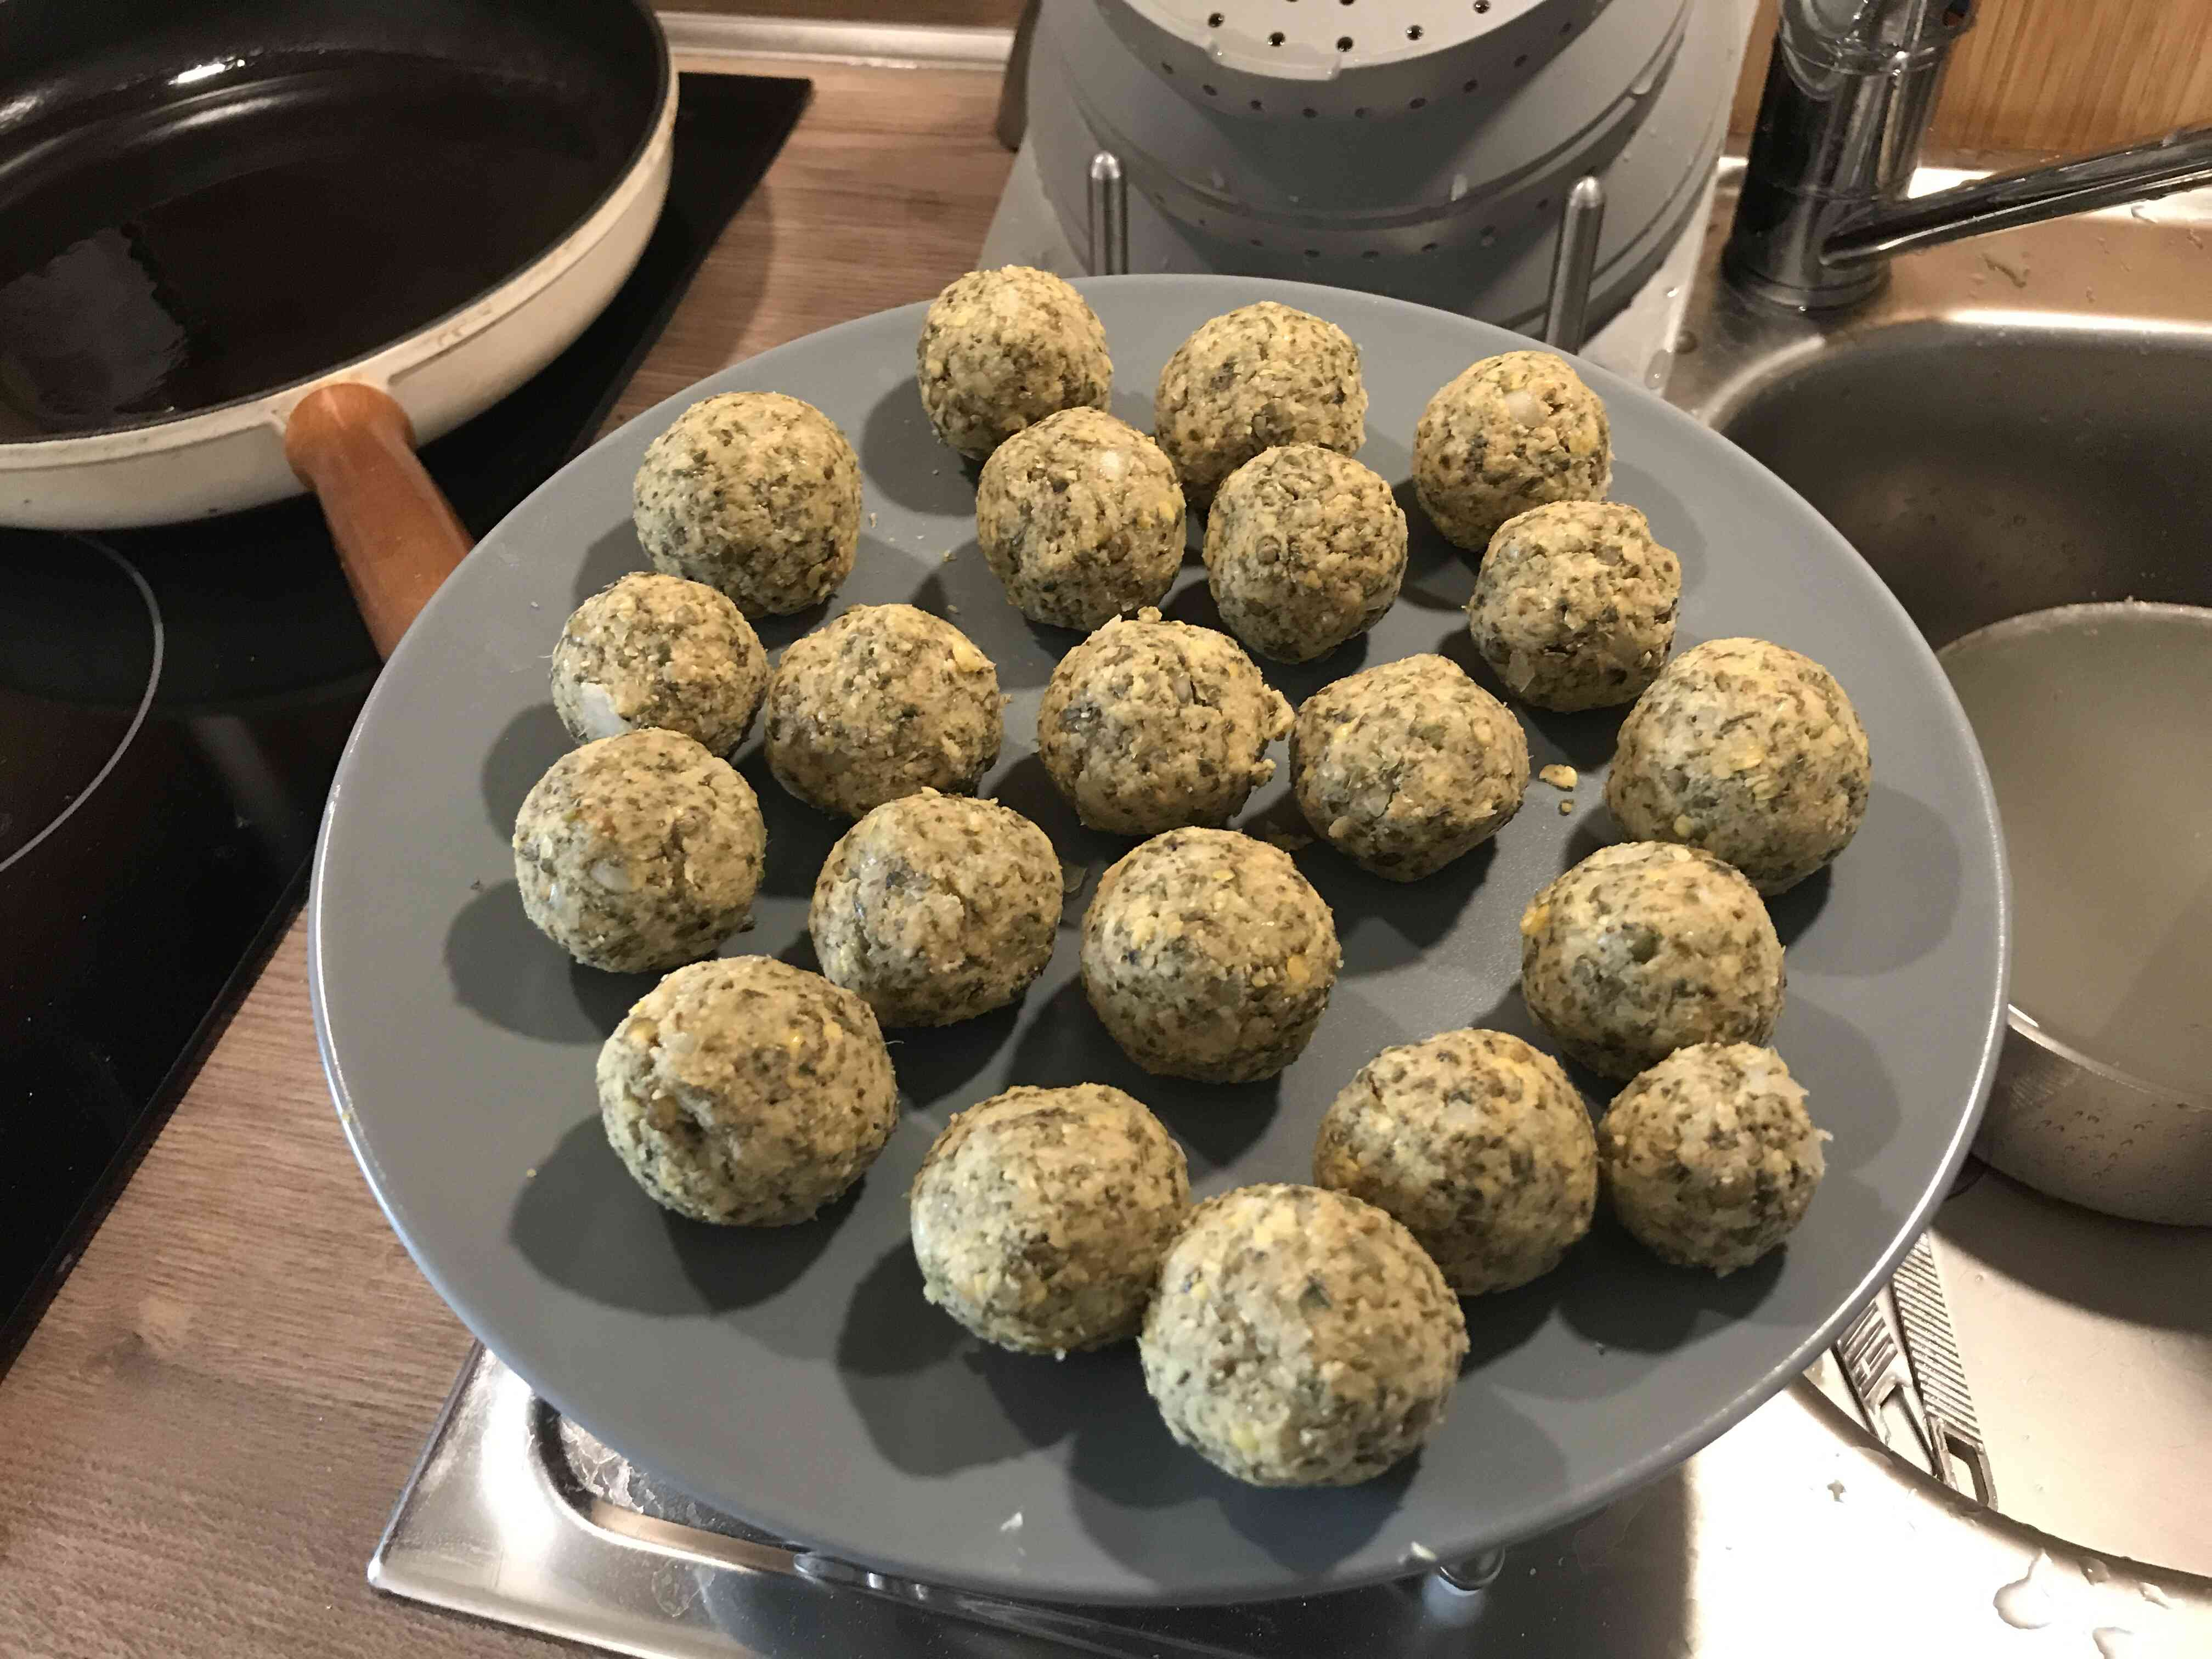
\includegraphics[width = \textwidth]{media/Falaffel.JPG}
		\caption{Falaffel aus grünen Linsen}
	\end{figure}
	\newpage

	% Couscous

	\section{Couscous}

	\begin{tabularx}{\textwidth}{r|L}
		%						& 	\includegraphics{\media\vorlage.jpg}	\\
		\textbf{Beschreibung}	&	Die wahrscheinlich schnellste Kohlenhydratquelle zum Zubereiten.\\
								&	\\
		\begin{tabular}[t]{rr}
			\textbf{Zutaten}	\\
			Für 800 g 			\\
			Für 4 Portionen	\\
		\end{tabular}			&	\begin{tabular}[t]{llll}
										400 g & $:= n$& Couscous \\	
										400 ml & $n$ g & Wasser	\\
										4 g	& n/100 G & Salz \\
										Gemüsebrühe/sonstige Würzung \\	
									\end{tabular}	\\
								&	\\
		\textbf{Variationen}	&	\begin{itemize}[nosep]
										\item Süßer Couscous?
									\end{itemize}	\\
								&	\\	
		\textbf{Passendes}		&	\begin{itemize}[nosep]
										\item Gemüse (Erbsen. Mais)
										\item Beilage als Proteinquelle
									\end{itemize}	\\
								&	\\	
		\begin{tabular}[t]{rr}
			\textbf{Zubereitung}	\\
			Arbeitszeit: 5-10 min	\\
		\end{tabular}			&	\begin{enumerate}[nosep]
										\item Bringe gesalzenes Wasser in einem Topf zum Kochen und füge optionale Würzung hinzu.
										\item Gib den Couscous hinzu, rühre gut um, nehme den Topf vom Herd und lasse den Couscous 5-10 min quellen.
									\end{enumerate}	\\
	\end{tabularx}
	\newpage

%----------------------------------<Beilagen>--------------------------------------

\chapter{Beilagen}

	% Gemüse in weiß

	\section{Angedünstetes Gemüse}

	\begin{tabularx}{\textwidth}{r|L}
								& 	\includegraphics[height = 5cm]{media/Lauchgemüse.JPG}	\\
								&	\\
		\textbf{Beschreibung}	&	Verschieden Gemüse können gut in kleinen Stücken mit ein wenig Sahne oder Schmand angedünstet werden, damit sie eine gute Beilage abgeben.\\
								&	\\
		\begin{tabular}[t]{rr}
			\textbf{Zutaten}	\\
			Für 500 g 			\\
			Für 4 Portionen	\\
		\end{tabular}			&	\begin{tabular}[t]{llll}
										400 g 	& Lauch, Brokkoli, Möhren, Zucchini \\
										100 g	& Sahne/Schmand/Creme Fraîche  \\	
										Salz, Pfeffer \\							
									\end{tabular}	\\
								&	\\
		\textbf{Variationen}	&	\begin{itemize}[nosep]
										\item ...
									\end{itemize}	\\
								&	\\	
		\textbf{Passendes}		&	\begin{itemize}[nosep]
										\item Reis
										\item Kartoffeln
										\item Spätzle
									\end{itemize}	\\
								&	\\	
		\begin{tabular}[t]{rr}
			\textbf{Zubereitung}	\\
			Arbeitszeit: 10 min	\\
			Gesamtzeit:	30 min		\\
		\end{tabular}			&	\begin{enumerate}[nosep]
										\item Schneide das Gemüse in kleine gleichgroße Stücke
										\item Erhitze ein wenig Öl in einem Topf und brate das Gemüse zuerst leicht an
										\item Gib das Milchprodukt der Wahl hinzu und würze mit ein wenig Salz und Pfeffer
										\item Decke anschließend zum Kochen 15-20 min den Topf mit dem Deckel zu
										\item Überprüfe die Konsistenz
									\end{enumerate}	\\
	\end{tabularx}
	\newpage

	% Bohnen

	\section{Stangenbohnen}	\label{stangenbohnen}

	\begin{tabularx}{\textwidth}{r|L}
		%						& 	\includegraphics[height = 5cm]{media/vorlage.jpg}	\\
		%						&	\\
		\textbf{Beschreibung}	&	Lange Bohnen, meist grün, von denen man die Schote andünsten kann.\\
								&	\\
		\begin{tabular}[t]{rr}
			\textbf{Zutaten}	\\
			Für 600 g 			\\
			Für 4-6 Portionen	\\
		\end{tabular}			&	\begin{tabular}[t]{llll}
										500 g & Bohnen \\
										2 & Zwiebeln \\
										2 Zehen & Knoblauch \\
										3 Zweige & Bohnenkraut! \\
										etwas Wasser \\
										Salz, Pfeffer \\								
									\end{tabular}	\\
								&	\\
		\textbf{Variationen}	&	\begin{itemize}[nosep]
										\item ...
									\end{itemize}	\\
								&	\\	
		\textbf{Passendes}		&	\begin{itemize}[nosep]
										\item Kartoffeln
										\item Fleisch
									\end{itemize}	\\
								&	\\	
		\begin{tabular}[t]{rr}
			\textbf{Zubereitung}	\\
			Vorbereitungszeit: 15 min	\\
			Garzeit:	20-30 min		\\
		\end{tabular}			&	\begin{enumerate}[nosep]
										\item Wasche die Bohnen und schneide die beiden harten Enden ab.
										\item Schneide die Zwiebeln und den Knoblauch in kleine Würfel.
										\item Brate die Zwiebeln in einer Pfanne mit ordentlich Öl glasig.
										\item Füge das Bohenkraut, den Knoblauch, Salz, Pfeffer und etwas Wasser hinzu und lasse alles bei geschlossenem Deckel dünsten bei mittlerer Hitze, bis die gewünschte Konsistenz erreicht ist.
									\end{enumerate}	\\
	\end{tabularx}
	\newpage

	% Seitan

	\section{Seitan}	\label{seitan}

	\begin{tabularx}{\textwidth}{r|L}
								& 	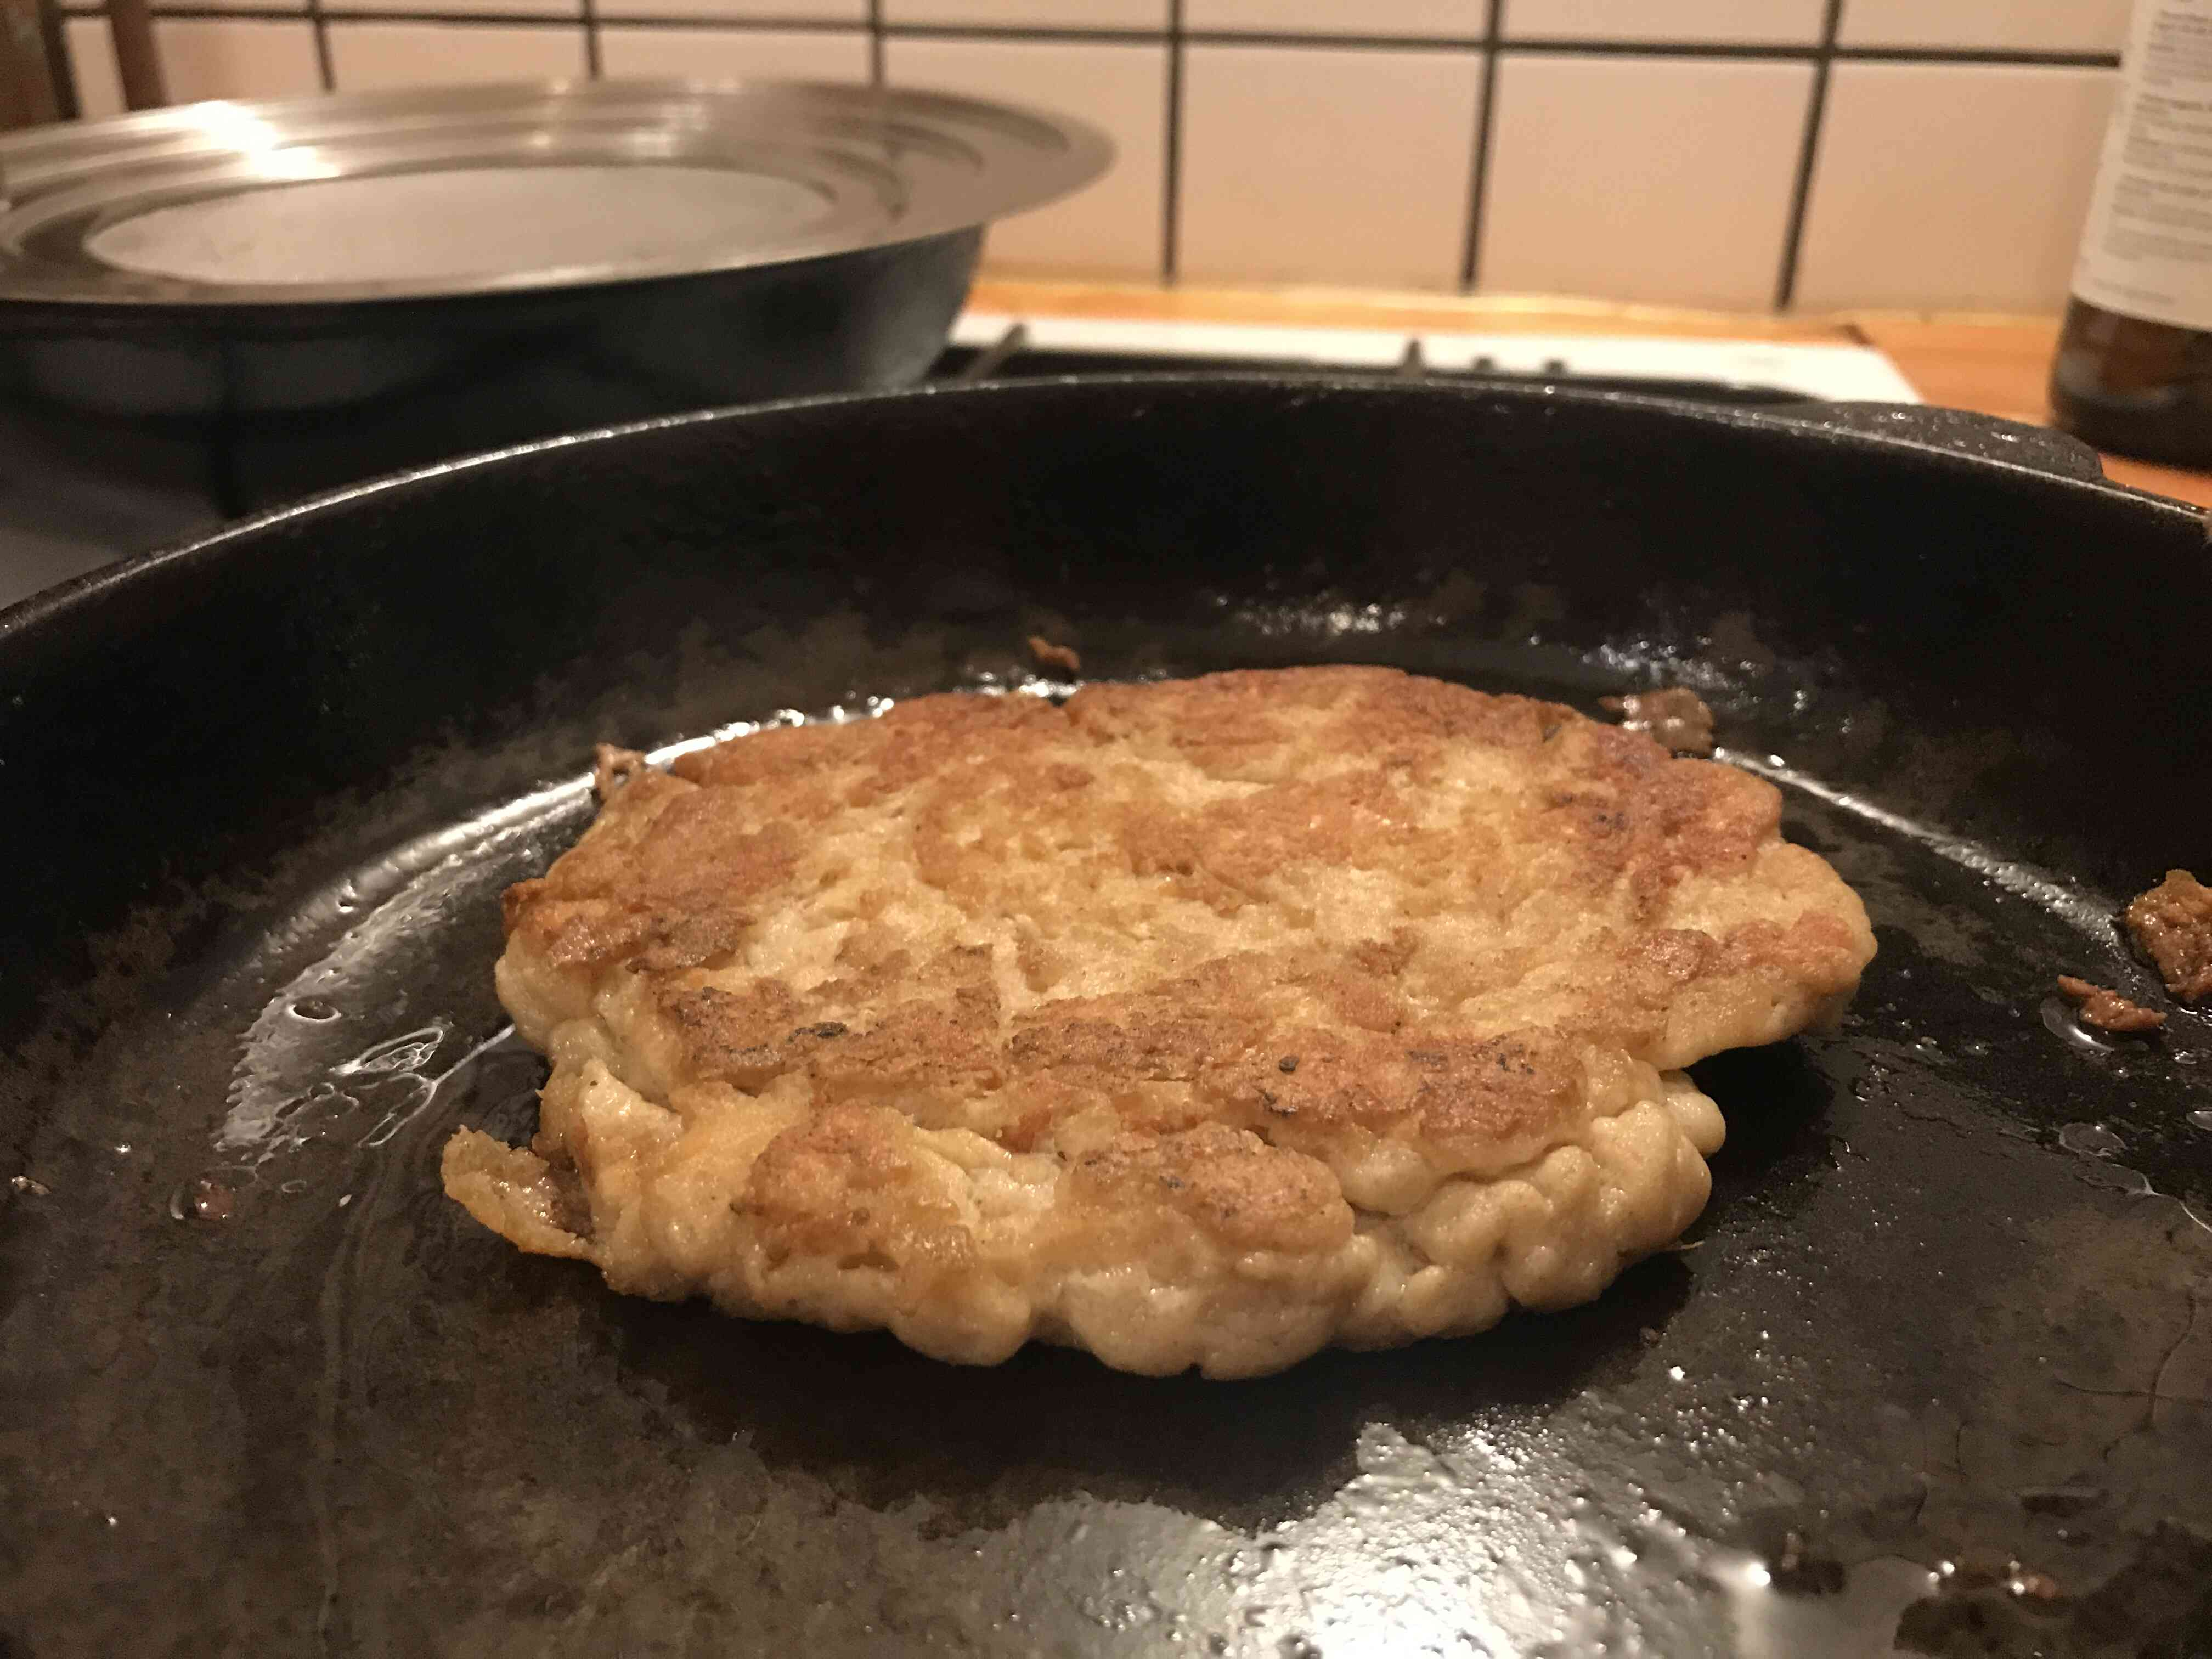
\includegraphics[height = 5cm]{media/seitan.JPG}	\\
								&	\\
		\textbf{Beschreibung}	&	Aus der asiatischen Küche kommt dieser Meister der Variabilität.  \\ 
								&	Sowohl die Konsistenz als auch den Geschmack kann man so unterschiedlich einstellen, das jedes Stück Fleisch neidisch werden sollte. \\
								&	Seitan kann sehr gut auf Vorrat zubereitet werden und dann ein paar Tage im Kühlschrank oder ein paar Wochen im Tiefkühlfach aufbewahrt werden.\\
								&	\\
		\begin{tabular}[t]{rr}
			\textbf{Zutaten}	\\
			Für 400 g 			\\
			Für 4 Portionen	\\
		\end{tabular}			&	\begin{tabular}[t]{llll}
										200 ? g & Weizengluten \\
										200 ml & Wasser \\
										20 ml & Öl \\
										6 ? g & Salz \\							
									\end{tabular}	\\
								&	\\
		\textbf{Variationen}	&	\begin{itemize}[nosep]
										\item Mediterrane Würzung: Olivenöl, Rosmarin, Oregano, Thymian
										\item Asiatische Würzung: Knoblauch, Ingwer, Sojasoße
										\item Indische Würzung: Kurkuma, Koriander, Kreuzkümmel, Paprikapulver, Chilipulver
										\item Standard Würzung: Pfeffer, wenig Knoblauch, Paprikapulver, Chilipulver, Gemüsebrühe
									\end{itemize}	\\
								&	\\	
		\textbf{Passendes}		&	\begin{itemize}[nosep]
										\item Burger
										\item Reis, Couscous
										\item Soßen
										\item Tortillas
									\end{itemize}	\\
								&	\\	
	\end{tabularx}

	\newpage
	\begin{tabularx}{\textwidth}{r|L}
		\begin{tabular}[t]{rr}
			\textbf{Zubereitung}	\\
			Arbeitszeit: 15 min	\\
			Gesamtzeit:	30-45 min \\
		\end{tabular}			&	\begin{enumerate}[nosep]
											\item Mische zu allererst das Glutenmehl mit der gewünschten Würzung gleichmäßig.
											\item Gib nun unter das Wasser hinzu und rühre alles gut durch. Es sollte ein sehr elastischer Kaugummi-artiger Teig entstehen.
											\item Gare den rohen Seitan indem du eines der Gar-Verfahren durchführt
											\begin{itemize}
												\item Im Kochtopf für eine zarte lockere weiche Konsistenz
												\begin{itemize}
													\item Schneide den rohen Seitan in kleinere Stücke.
													\item Koche den Seitan in gesalzenem Wasser für 30 min.
												\end{itemize}
												\item Zubereitung in Pfanne
												\begin{itemize}
													\item Gib den rohen Seitan in ein Pfanne mit etwas gesalzenem Wasser am Boden und koche ihn für 20-30 min.
													\item Gieße anschließend das Wasser ab und braten den Seitan an.
												\end{itemize}
												\item Im Ofen für eine weiche kompakte Konsistenz
												\begin{itemize}
													\item Gib den rohen Seitan in eine Backform.
													\item Backe ihn für 30 min bei 180°C?
												\end{itemize}
												\item In der Mikrowelle zum schnellen Garen
												\begin{itemize}
													\item auch möglich in der Mikrowelle bei 360W für 5 min ?
												\end{itemize}
											\end{itemize}
													
									\end{enumerate}	\\
	\end{tabularx}
	\newpage


	% Falaffel

	\section{Falaffel}	\label{Falaffel}

	\begin{tabularx}{\textwidth}{r|L}
								& 	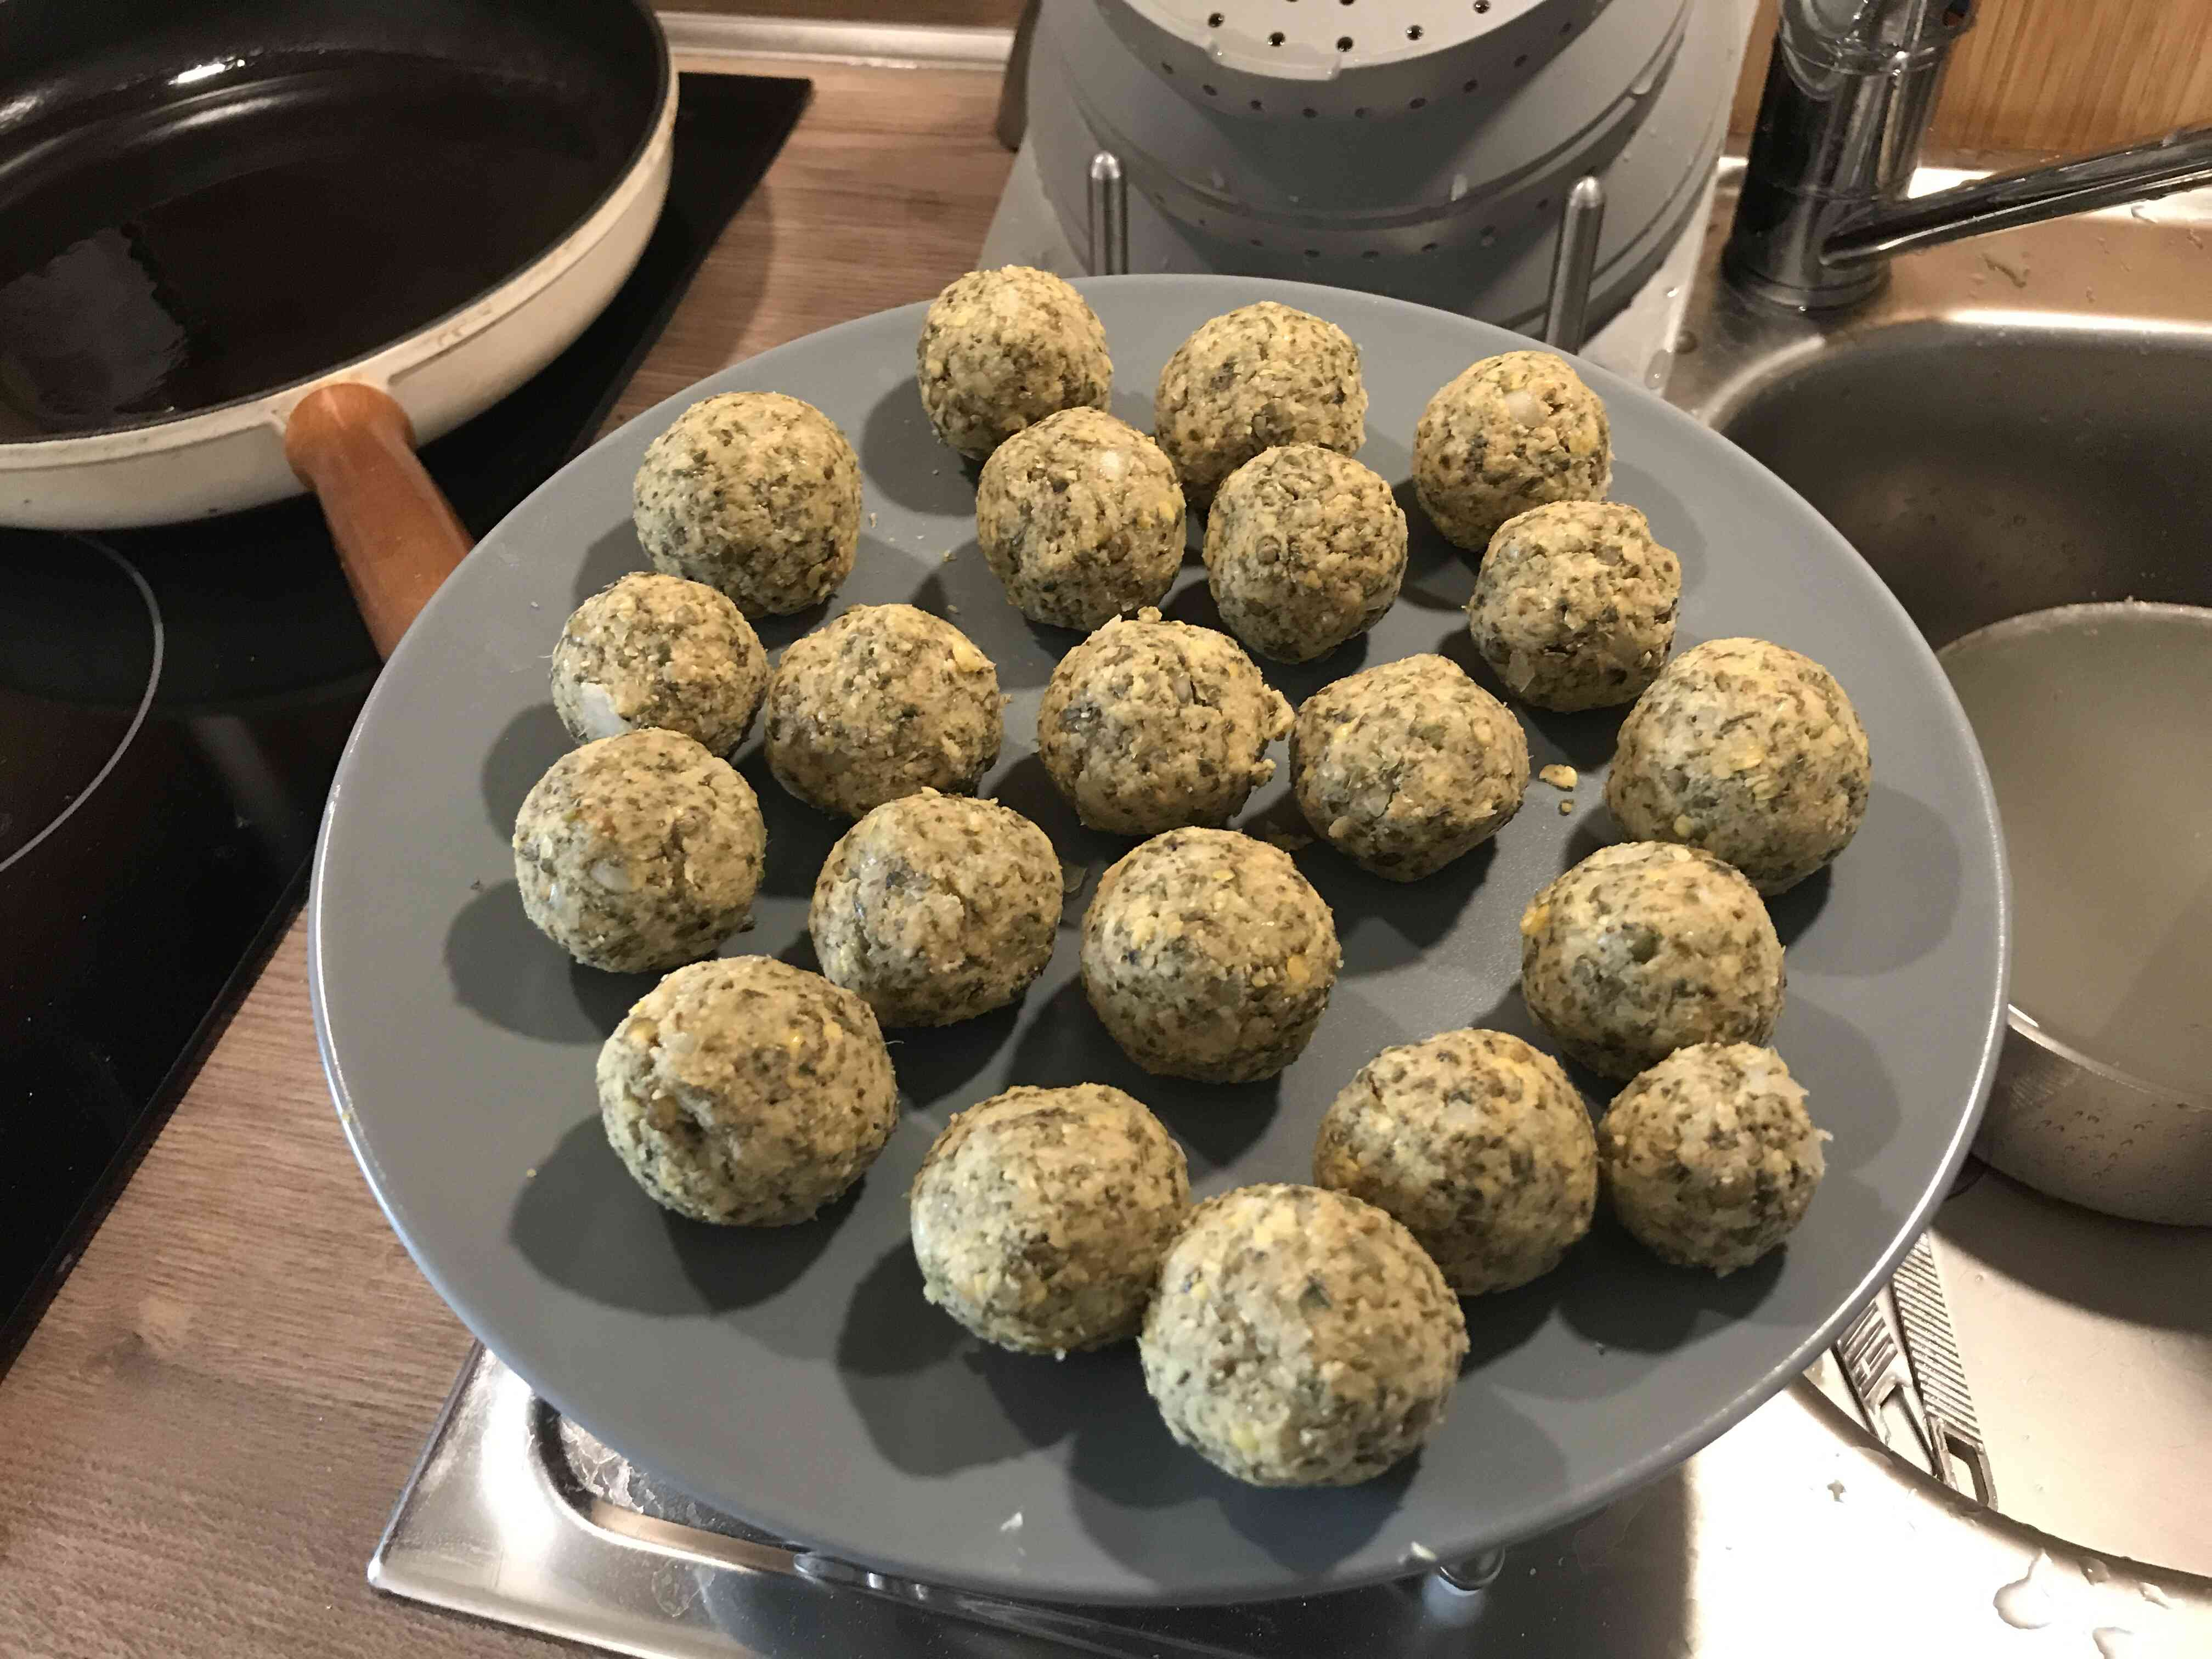
\includegraphics[height = 5cm]{media/Falaffel.JPG}	\\
								&	\\
		\textbf{Beschreibung}	&	Eine vegane würzige Knusprigkeit\\
								&	\\
		\begin{tabular}[t]{rr}
			\textbf{Zutaten}	\\
			Für ... g 			\\
			Für ... Portionen	\\
		\end{tabular}			&	\begin{tabular}[t]{llll}
										200 g & Kichererbsen \\
										20 g & Mehl \\
										3 g & Salz \\
										Würzungen \\		
									\end{tabular}	\\
								&	\\
		\textbf{Variationen}	&	\begin{itemize}[nosep]
										\item Standard-Würzung: Kräuter, Petersilie, Chili, Knoblauch, Zwiebeln
									\end{itemize}	\\
								&	\\	
		\textbf{Passendes}		&	\begin{itemize}[nosep]
										\item Reis
										\item Pita-Brot
									\end{itemize}	\\
								&	\\	
		\begin{tabular}[t]{rr}
			\textbf{Zubereitung}	\\
			Arbeitszeit: ...	\\
			Gesamtzeit:	...		\\
		\end{tabular}			&	\begin{enumerate}[nosep]
										\item Püriere die gekochten Kichererbsen möglichst fein in einem hohen Gefäß.
										\item Würze die Masse und verknetet alles.
										\item Gib so viel Mehl hinzu, sodass eine gut formbare Masse entsteht.
										\item Mit angefeuchteten Händen können unter Druck kleine Falaffel gedreht werden.
										\item Gib die rohen Falaffel in eine Pfanne mit ordentlich Öl und brate sie für 3-5 min unter regelmäßigem Schwenken.
										\item ACHTUNG! Die warmen Falaffel sind äußerst fragil und sollten nicht mit einem Pfannenschaber konfrontiert werden.
										\item Wenn der gewünschte Bräunungsgrad erreicht ist, lasse die Falaffel außerhalb der Pfanne abkühlen.
									\end{enumerate}	\\
	\end{tabularx}
	\newpage

	% Gemüse-Bratlinge

	\section{Gemüse-Bratlinge}	\label{gemuese_bratlinge}

	\begin{tabularx}{\textwidth}{r|L}
								& 	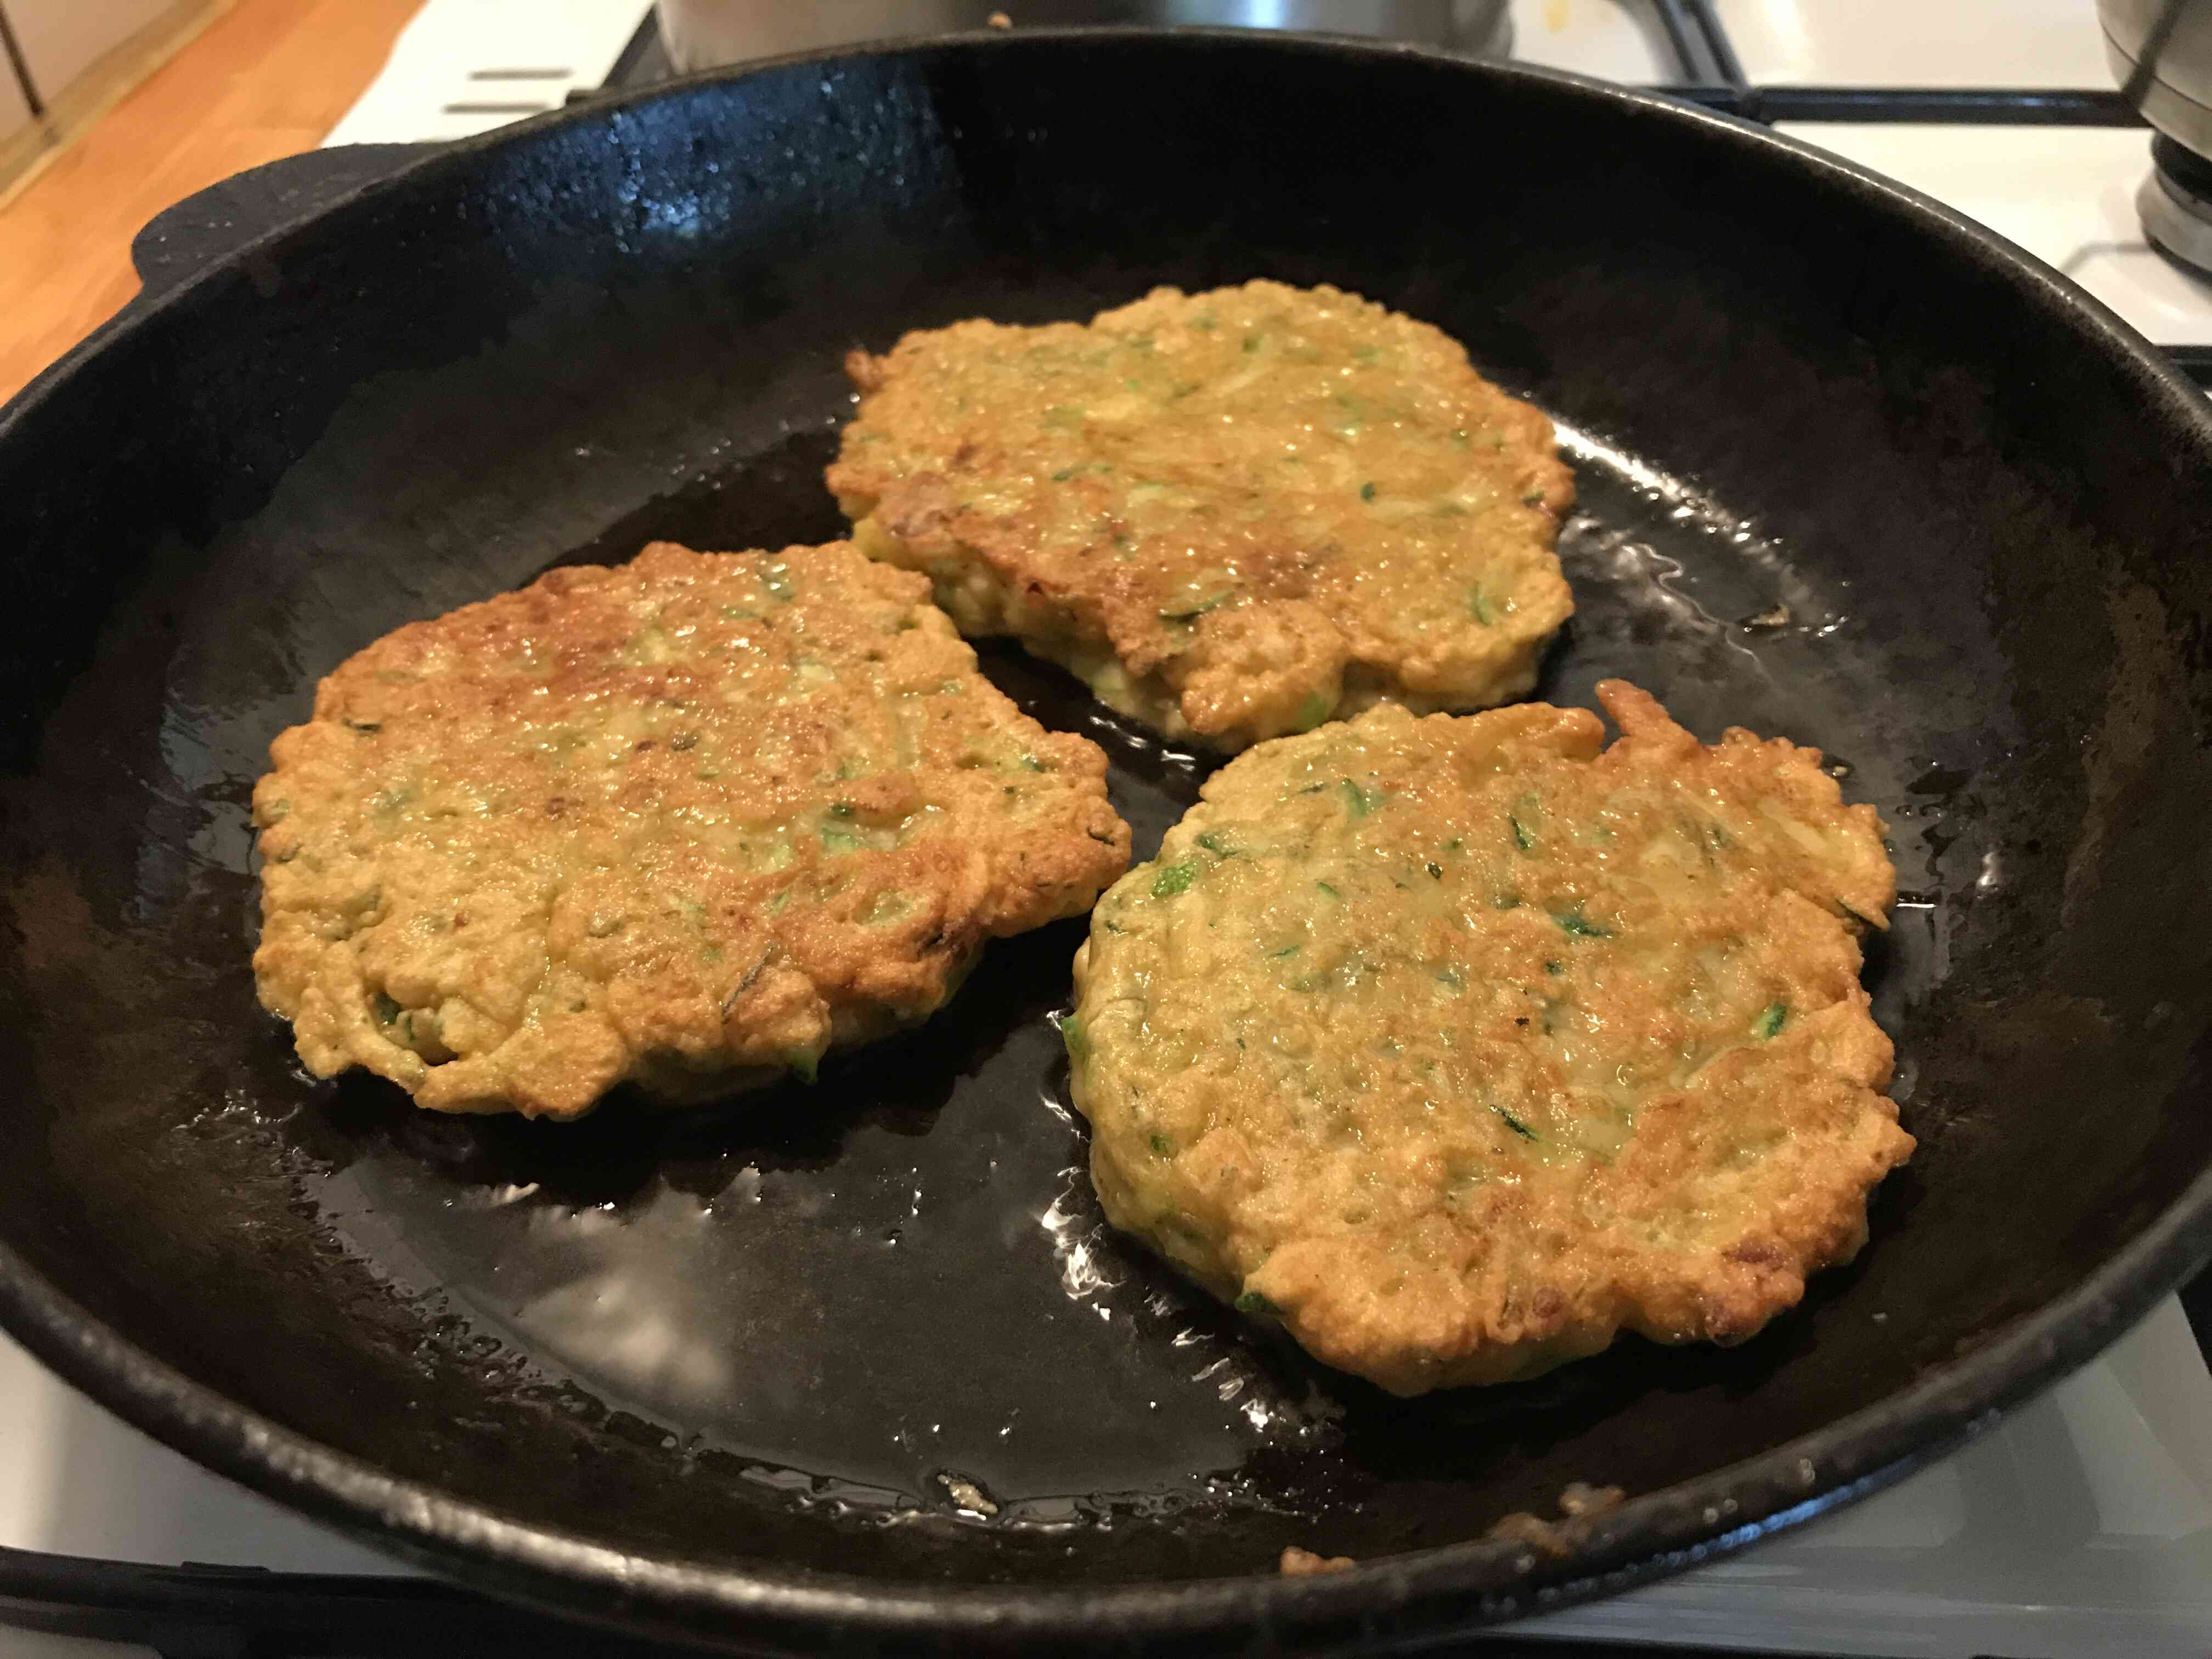
\includegraphics[height = 5cm]{media/zucchini_bratling.JPG}	\\
								&	\\
		\textbf{Beschreibung}	&	Eine Art Gemüse zu verpacken, die selbst meinem kleinen Bruder geschmeckt hat. Es erinnert oftmals sehr an Kartoffelpuffer, aber kann deutlich variabler gehandhabt werden. \\
								&	\\
		\begin{tabular}[t]{rr}
			\textbf{Zutaten}	\\
			Für 1,8 kg 			\\
			Für 10-15 Portionen	\\
		\end{tabular}			&	\begin{tabular}[t]{llll}
										1 kg & Gemüse, geraspelt oder klein geschnitten: \\
											 & - Zwiebeln \\			
											 & - Zucchini, Möhre, Kohlrabi, Brokkoli \\
										4 & Eier \\
										250 g & Mehl \\
										7 g & Salz \\
										& Pfeffer \\
										& Gewürze: Kurkuma, Koriander, Paprikapulver, Piment \\			
									\end{tabular}	\\
								&	\\
		\textbf{Variationen}	&	\begin{itemize}[nosep]
										\item ...
									\end{itemize}	\\
								&	\\	
		\textbf{Passendes}		&	\begin{itemize}[nosep]
										\item Joghurt-Dip 
										\item Kräuterquark
										\item Bratling im Burger
										\item Reis
									\end{itemize}	\\
								&	\\
	\end{tabularx}

	\begin{tabularx}{\textwidth}{r|L}
		\begin{tabular}[t]{rr}
			\textbf{Zubereitung}	\\
			Vorbereitungszeit: 30 min	\\
			Garzeit: 20-30 min		\\
		\end{tabular}			&	\begin{enumerate}[nosep]
										\item Reibe oder schneide das Gemüse möglichst fein und gib alles in eine große Schüssel.
										\item Gibt die Eier, das Mehl, das Salz und die Gewürze hinzu und mische alles gut unter, sodass einer gleichmäßiger Teig entsteht.
										\item Erhitze eine oder mehrere Pfannen mit ordentlich Bratöl und gib vier mal 1-2 EL des Teiges in jede Pfanne.
										\item Wende die Bratlinge, wenn die ersten angerösteten Stellen sichtbar sind.
									\end{enumerate}	\\
	\end{tabularx}
	\newpage

	\section{Aufstriche}

%----------------------------------<Soßen>--------------------------------------

\chapter{Sauce}

	% Béchamelsoße 

	\section{Béchamelsauce}

	\begin{tabularx}{\textwidth}{r|L}
								& 	\includegraphics[height = 5cm]{media/bechamelsoße.png}	\\
		\textbf{Beschreibung}	&	Die helle Grundsoße, welche als Ausgangspunkt für viele andere Soßen dienen kann. Mit \textit{Nudeln mit heller Soße} verbinde ich noch immer meine Kindheit.\\
								&	\\
		\begin{tabular}[t]{rr}
			\textbf{Zutaten}	\\
			Für 300 g 			\\
			Für 2-4 Portionen	\\
		\end{tabular}			&	\begin{tabular}[t]{llll}
										250 ml & Milch \\
										20 g & Mehl	\\
										20 g & Butter \\
										5 g & Salz \\								
									\end{tabular}	\\
								&	\\
		\textbf{Variationen}	&	\begin{itemize}[nosep]
										\item \textit{Weiße Soße} mit weißem Pfeffer und Muskat
										\item \textit{Käsesoße} mit 50-100 g Cheddar, Gouda oder Gorgonzola 
									\end{itemize}	\\
								&	\\	
		\textbf{Passendes}		&	\begin{itemize}[nosep]
										\item Nudeln
										\item Spätzle
									\end{itemize}	\\
								&	\\	
		\begin{tabular}[t]{rr}
			\textbf{Zubereitung}	\\
			Arbeitszeit: 5-10 min		\\
		\end{tabular}			&	\begin{enumerate}[nosep]
										\item Gib die Butter in einem Topf, lasse sie schmelzen und füge bei niedriger Hitze und ständigem Rühren das Mehl hinzu. Der Arbeitsschritt nennt sich Mehlschwitze.
										\item Gib die Milch hinzu und rühre, bis die Soße anfängt zu kochen.
										\item Koche sie für ein paar Minuten, da der Mehlgeschmack hiermit verschwinden soll.
										\item Würze sie mit dem Salz und Pfeffer, bis der gewünschte Geschmack erreicht ist. 
									\end{enumerate}	\\
	\end{tabularx}
	\newpage


	% Pesto

	\section{Pesto}	\label{pesto}

	\begin{tabularx}{\textwidth}{r|L}
								& 	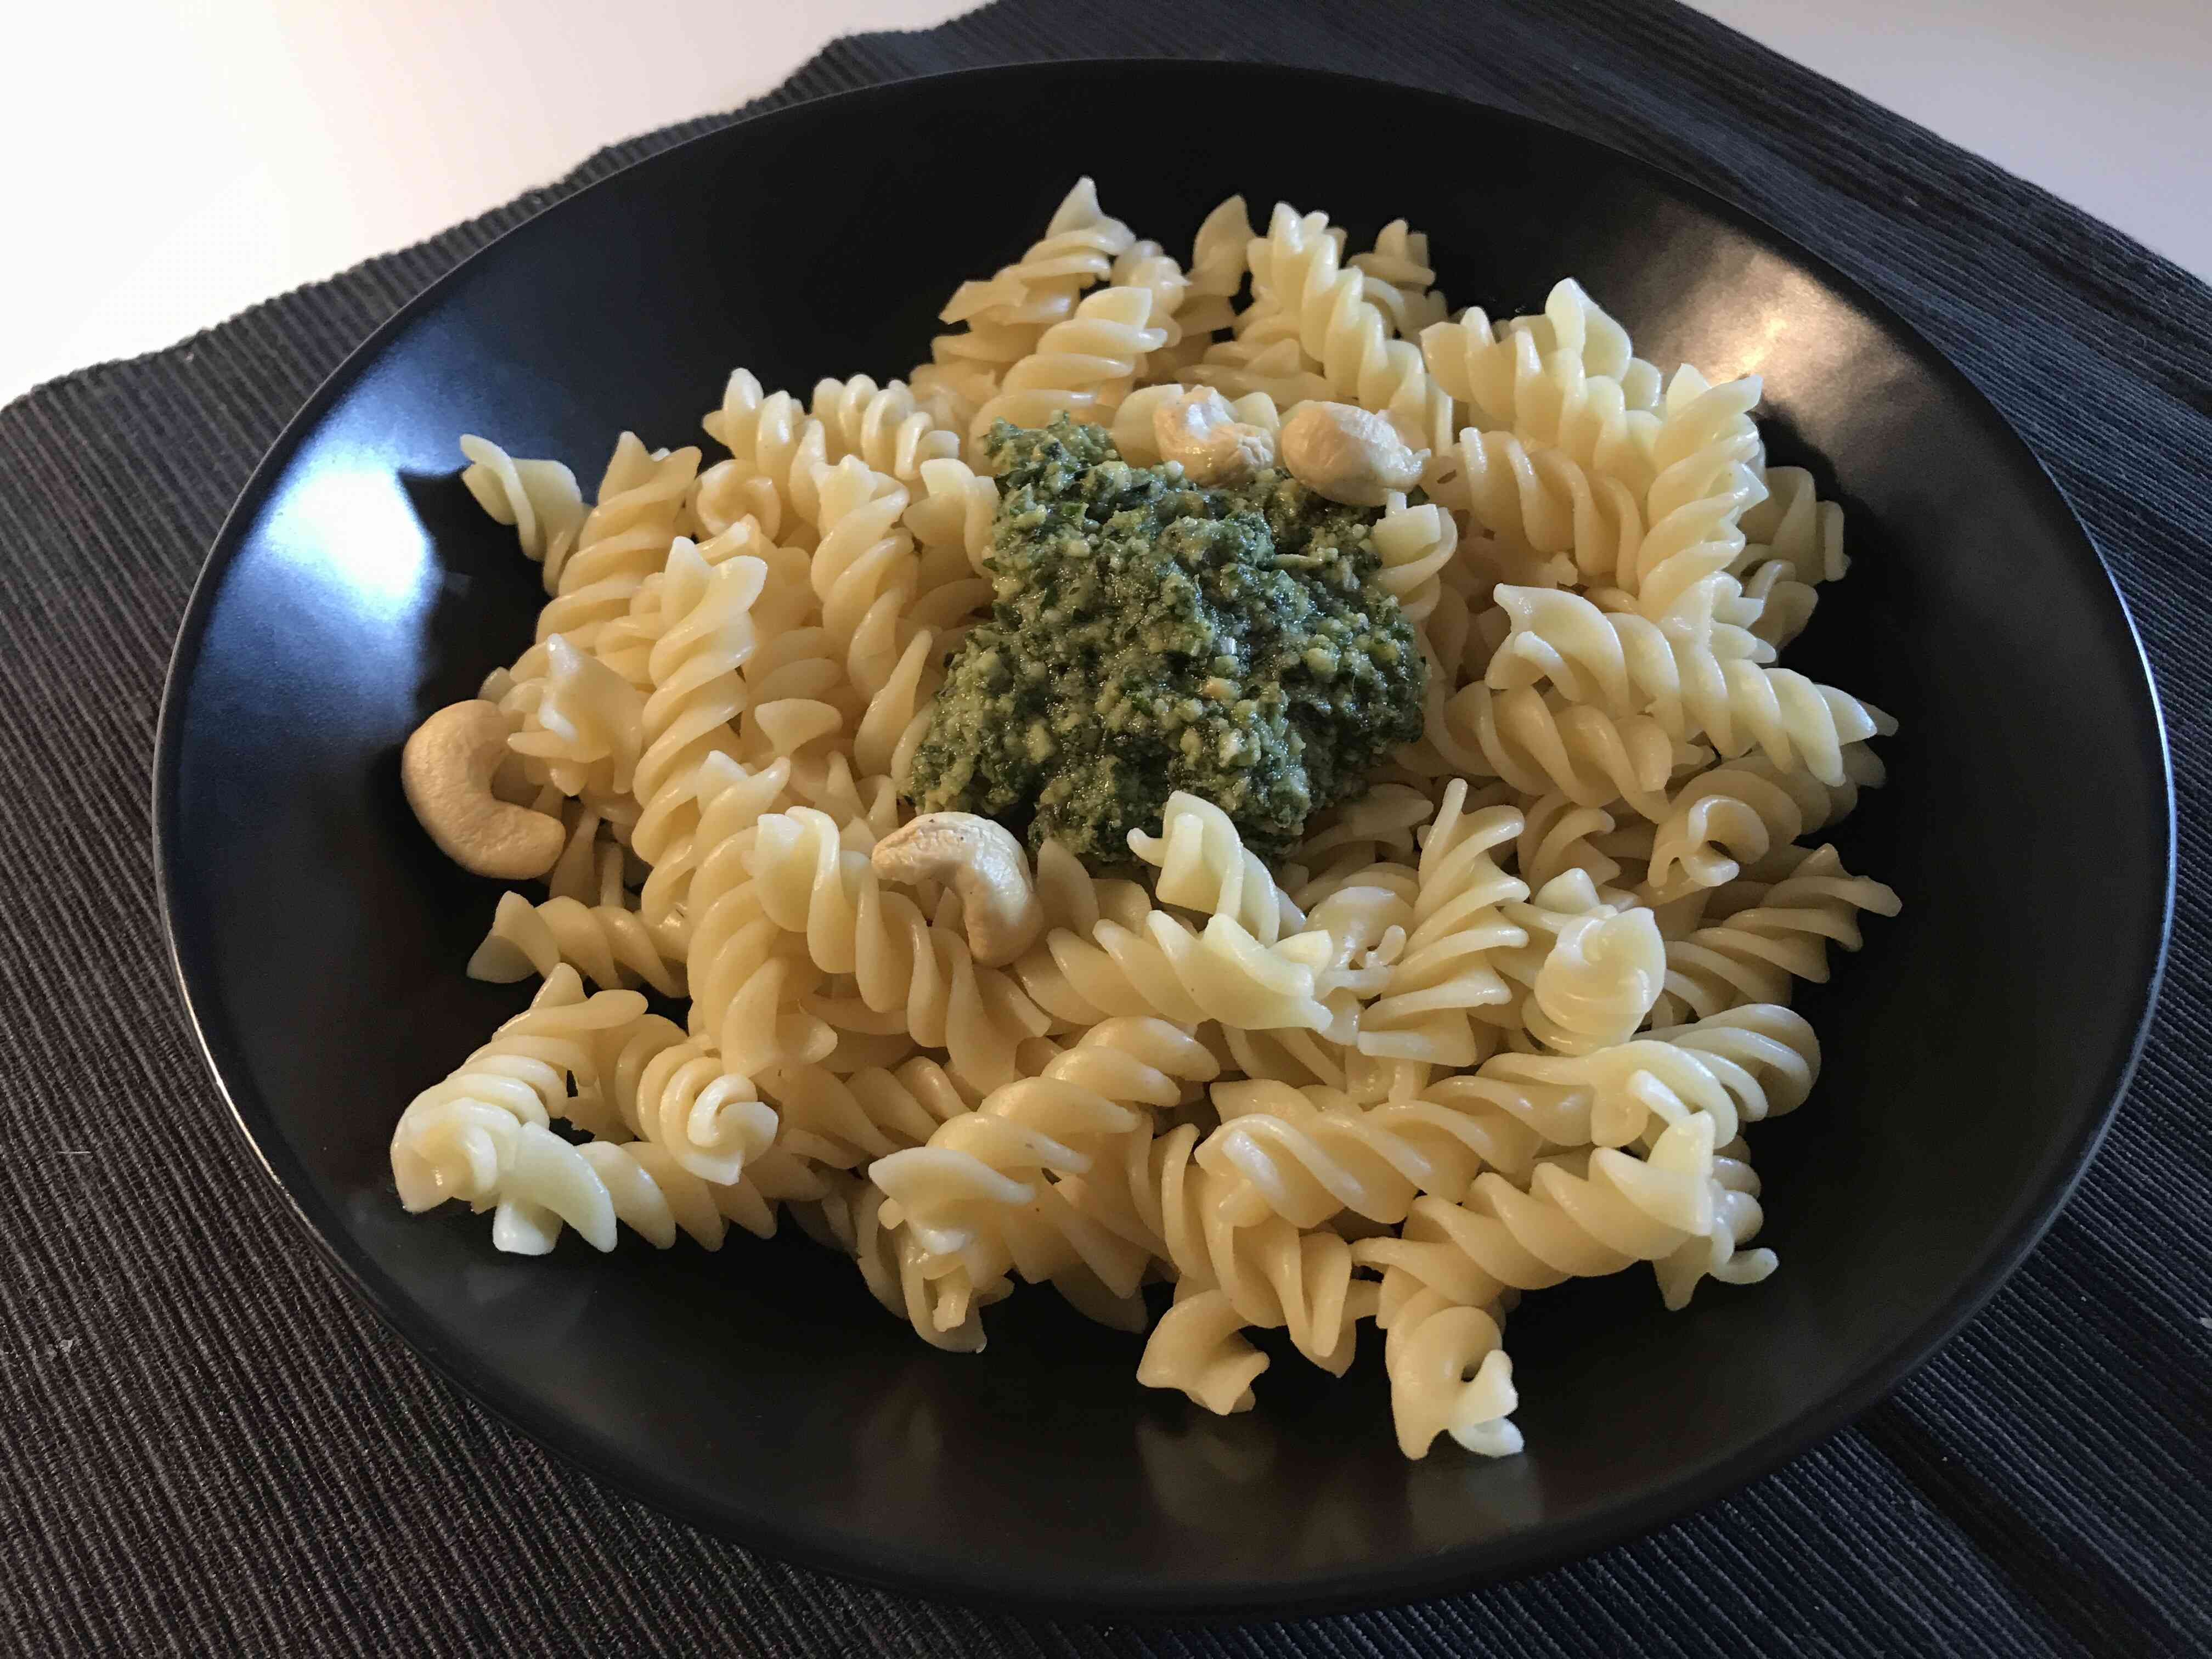
\includegraphics[height = 5cm]{media/pesto_nudeln.JPG}	\\
								&	\\
		\textbf{Beschreibung}	&	Eine italiensche ungekochte Würzsauce, welche ihren Namen durch das itl. Wort \emph{pestare} für \emph{zerstampfen} erhalten hat. \\
								&	\\
		\begin{tabular}[t]{rr}
			\textbf{Zutaten}	\\
			Für 150 g 			\\
			Für 3-4 Portionen	\\
		\end{tabular}			&	\begin{tabular}[t]{llll}
										Grünes Pesto: \\
											& 1 Strauch & Basilikum \\	
											& 50 ml & Olivenöl \\	
											& 40 g & Cashewkerne \\
											& 40 g & Parmesan \\
											& 2 Zehe & Knoblauch \\
											& 3 g & Salz						
									\end{tabular}	\\
								&	\\
		\textbf{Variationen}	&	\begin{itemize}[nosep]
										\item ...
									\end{itemize}	\\
								&	\\	
		\textbf{Passendes}		&	\begin{itemize}[nosep]
										\item Nudeln
									\end{itemize}	\\
								&	\\	
		\begin{tabular}[t]{rr}
			\textbf{Zubereitung}	\\
			Arbeitszeit: 15 min	\\
		\end{tabular}			&	\begin{enumerate}[nosep]
										\item Zupfe die Blätter des Basilikums von den Stängeln und wasche sie.
										\item Schäle den Knoblauch und gib alle Zutaten in ein Gefäß zum Pürieren.
										\item Püriere bis die gewünschte Konsistenz erreicht ist.
									\end{enumerate}	\\
	\end{tabularx}
	\newpage

	% Erdnuss-Kokos-Curry-Soße

	\section{Erdnuss-Kokos-Curry-Sauce}	\label{erdnuss_sauce}

	\begin{tabularx}{\textwidth}{r|L}
		%						& 	\includegraphics[height = 5cm]{media/vorlage.jpg}	\\
		%						&	\\
		\textbf{Beschreibung}	&	Eine intensive cremige Sauce zum Aufpeppen von Reisgerichten und anderen Beilagen.\\
								&	\\
		\begin{tabular}[t]{rr}
			\textbf{Zutaten}	\\
			Für 500 g 			\\
			Für 5-8 Portionen	\\
		\end{tabular}			&	\begin{tabular}[t]{llll}
										400 ml & Kokosmilch \\
										2 EL & Erdnussbutter \\
										1 TL & Stärke, in kaltem Wasser gelöst (zum Andicken)\\
										1 g & Salz \\
										Gewürze: & Kurkuma, Paprikapulver, Koriander, Piment, Cumin, ...\\							
									\end{tabular}	\\
								&	\\
		\textbf{Variationen}	&	\begin{itemize}[nosep]
										\item ...
									\end{itemize}	\\
								&	\\	
		\textbf{Passendes}		&	\begin{itemize}[nosep]
										\item Reis
									\end{itemize}	\\
								&	\\	
		\begin{tabular}[t]{rr}
			\textbf{Zubereitung}	\\
			Vorbereitungszeit: ...	\\
			Garzeit:	10 min		\\
		\end{tabular}			&	\begin{enumerate}[nosep]
										\item Gib die Kokosmilch in einen Kochtopf, erhitze ihn und löse die Erdnussbutter auf.
										\item Würze die Sauce und stelle die Konsistenz über Abkochen oder Andicken mit einer Stärkelösung ein.
									\end{enumerate}	\\
	\end{tabularx}
	\newpage

%----------------------------------<Fleisch>--------------------------------------

\chapter{Fleisch}

%----------------------------------<Vollständige Gerichte>--------------------------------------

\chapter{Vollständige Gerichte}
\newpage

	\section{Take-Away-Gerichte}
	\newpage

	\section{Käsespätzle}

	% hier sollte noch ein Bild hinein
	\noindent

	\begin{tabularx}{\textwidth}{r|L}
		\textbf{Beschreibung}	&	Ein wohlbekanntes Essen aus der Familie und von den FöJ-Seminaren.\\
								&	\\
		\begin{tabular}[t]{rr}
			\textbf{Zutaten}	\\
			Für 1,5 kg Käsespätzle	\\
			Für 4 Portionen		\\
		\end{tabular}			&	\begin{tabular}[t]{lll}
										500 g	&	Weizenmehl 550er	&	\\
										4-5		&	Eier				\\	
										300-400 g	&	Wasser				&	Wasser zu Mehl: $0,80 = 80\%$	\\
										10 g	&	Salz				&	Salz zu Wasser: $0,02 = 2\%$	\\
										250 g	&	Käse				\\	
										2-3		&	Zwiebeln				\\	
										200 g	&	Sahne		\\
										Petersilie	\\
									\end{tabular}	\\
								&	\\
		\textbf{Variationen}	&	\begin{itemize}[nosep]
										\item 1/3 Vollkorn und 2/3 550er Weizenmehl
									\end{itemize}	\\
								&	\\	
		\textbf{Passendes}		&	\begin{itemize}[nosep]
										\item Zwiebeln, angeröstet
									\end{itemize}	\\
								&	\\
% für zweiseitiges Rezept entkommentieren!
	\end{tabularx}
	\newpage
	\begin{tabularx}{\textwidth}{r|L}

		\begin{tabular}[t]{rr}
			\textbf{Zubereitung}	\\
			Arbeitszeit: 20-30 min	\\
			Gesamtzeit:	30-45 min	\\
		\end{tabular}			&	\begin{enumerate}[nosep]
										\item Setze mindestens 2 l Wasser zum Kochen auf.
										\item Verrühre Mehl, Salz, Eier und Wasser in einer Schüssel, so lange, bis der Teig Fäden zieht und nicht zu flüssig ist.
										\item Schneide die Zwiebel in Ringe und brate sie in einer Pfanne glasig an, mit Öl und ein wenig Salz.
										\item Gib die Teigmasse in einen Spätzlehobel oder auf ein Brett um die Spätzle herzustellen und lasse sie in das kochende Wasser fallen.
										\item Lasse die Spätzle kochen, bis die alle oben aufschwimmen und nehme sie schließlich mit einer Schöpfkelle ab.
										\item Gib die fertigen Spätzle in eine große Schüssel und wiederhole Schritt 4-5 bis der Teig aufgebraucht ist.
										\item Richte die Spätzle mit geriebenem Käse und Zwiebeln an.
									\end{enumerate}	\\
								&	\\
	\end{tabularx}
	\newpage

	% Frikassee

	\section{Frikassee}	\label{frikassee}

	\begin{tabularx}{\textwidth}{r|L}
								& 	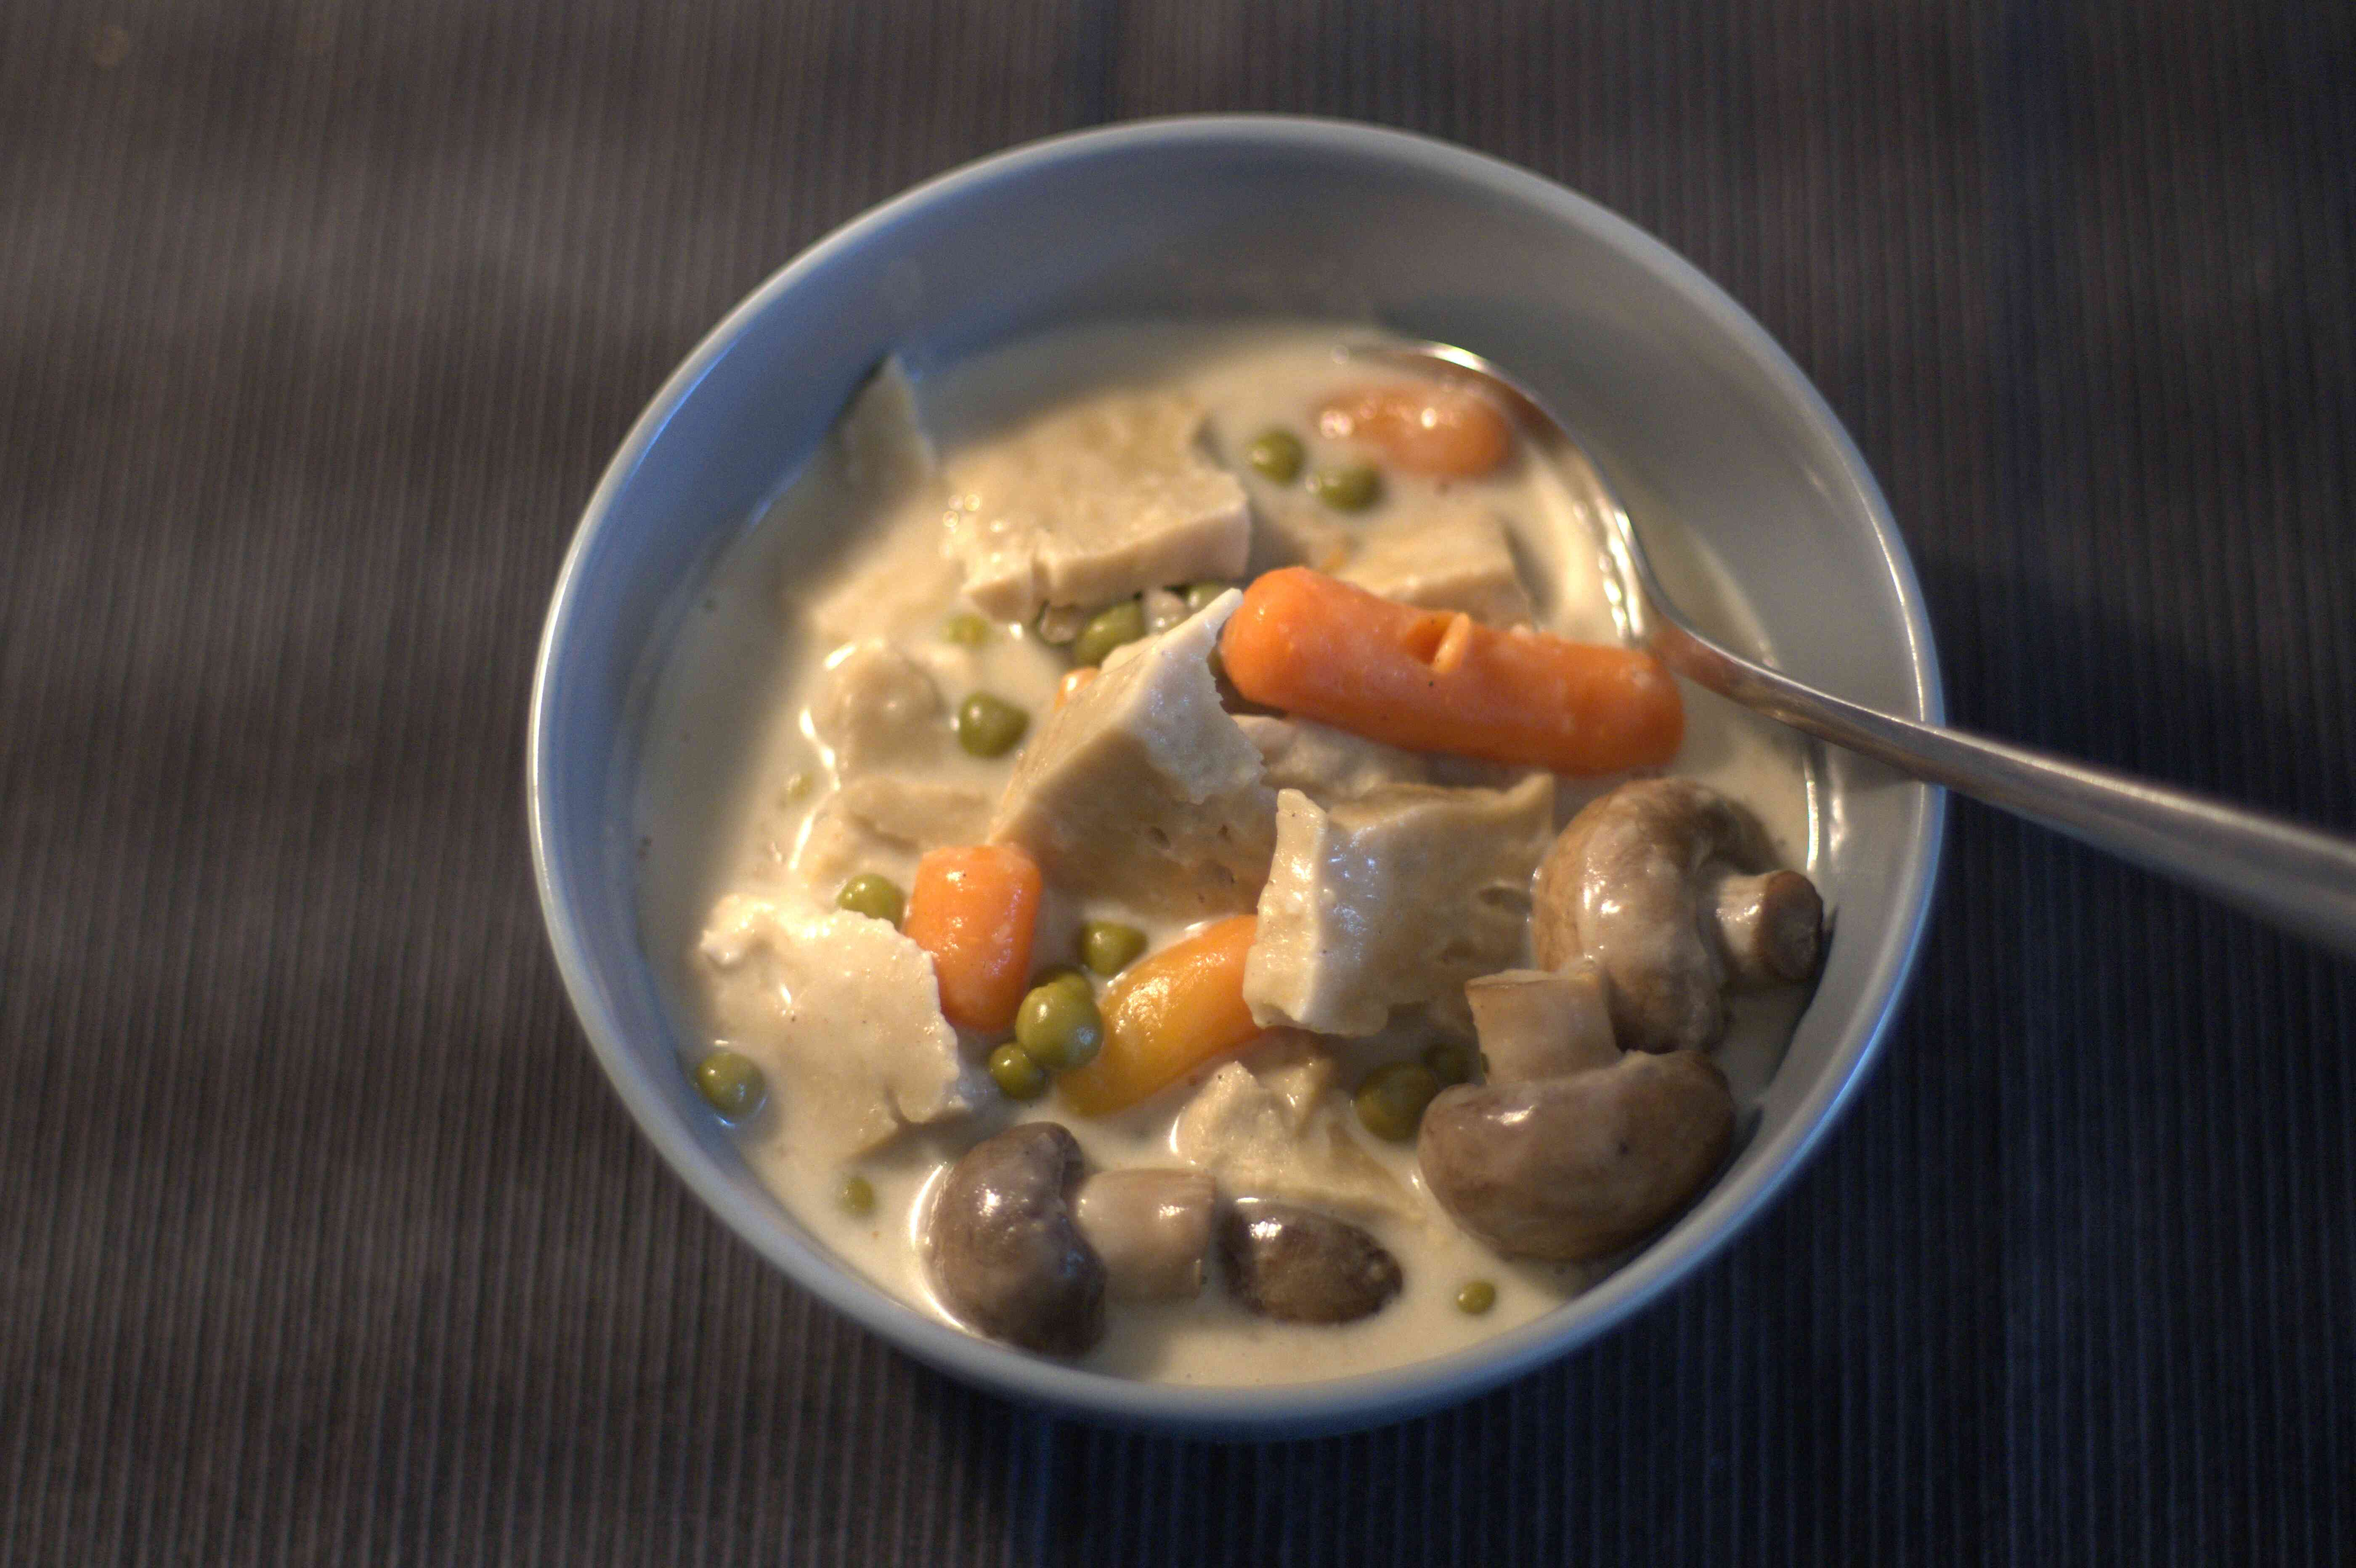
\includegraphics[height = 5cm]{media/frikasse.jpg}	\\
								&	\\
		\textbf{Beschreibung}	&	Eine cremige Kombination aus Fleisch, Pilzen, Erbsen und Möhren.\\
								&	\\
		\begin{tabular}[t]{rr}
			\textbf{Zutaten}	\\
			Für ... g 			\\
			Für 4 Portionen	\\
		\end{tabular}			&	\begin{tabular}[t]{llll}
										500 g & Hühnerbrust/Schweinefleisch/Seitan \\
										300 g & Champignons \\
										300 g & Erbsen und Möhren aus dem Glas \\
										2 TL & Brühepulver \\
										1 L & Wasser \\
										250 ml & Sahne/Schmand \\
										Salz, Pfeffer, Muskat \\
										\\
										Für Mehlschwitze: \\
										20 g & Butter \\
										2 EL & Mehl \\
									\end{tabular}	\\
								&	\\
		\textbf{Variationen}	&	\begin{itemize}[nosep]
										\item ...
									\end{itemize}	\\
								&	\\	
		\textbf{Passendes}		&	\begin{itemize}[nosep]
										\item Reis
										\item Nudeln
									\end{itemize}	\\
								&	\\	
% für zweiseitiges Rezept entkommentieren!
	\end{tabularx}
	\newpage
	\begin{tabularx}{\textwidth}{r|L}

		\begin{tabular}[t]{rr}
			\textbf{Zubereitung}	\\
			Arbeitszeit: 30 min	\\
			Gesamtzeit:	10-20 min	\\
		\end{tabular}			&	\begin{enumerate}[nosep]
										\item Das Fleisch oder den Seitan schneiden und falls nötig in der Brühe kochen. 
										\item Die Brühe abfüllen und eine Mehlschwitze im Topf ansetzen.
										\item Nun die Brühe unter Rühren wieder hinzugeben und die Champignons 15 min kochen lassen.
										\item Schneide das Fleisch oder den Seitan in Stücke und gib den Seitan, Erbsen und Möhren hinzu.
										\item Schmecke ab und würze das Frikassee final.
									\end{enumerate}	\\
	\end{tabularx}
	\newpage


	\section{Suppen}
	\newpage

		% Kartoffelsuppe

		\subsection{Kartoffel-Lauch-Suppe}

		\begin{tabularx}{\textwidth}{r|L}
			%						& 	\includegraphics[height = 5cm]{media/vorlage.jpg}	\\
			%						&	\\
			\textbf{Beschreibung}	&	Zum Verarbeiten des typischen Gemüse, was quasi immer verfügbar ist. Die Kartoffelsuppe ist definitiv eine familiäre Tradition ist bei meiner Mutter und ihrer Mutter. \\
									&	\\
			\begin{tabular}[t]{rr}
				\textbf{Zutaten}	\\
				Für 1,8 kg 			\\
				Für 4-6 Portionen	\\
			\end{tabular}			&	\begin{tabular}[t]{llll}
											1 kg & Kartoffel, geschält und gewürfelt \\
											2 Stangen & Lauch \\
											4 & Karotten \\
											1 L & Wasser \\
											1 EL & Gemüsebrühe/Hühnerbrühe \\
											& Schuss Sahne/Milch \\
											& Salz, Pfeffer \\
											& Petersilie, Lorbeer, Majoran \\								
										\end{tabular}	\\
									&	\\
			\textbf{Variationen}	&	\begin{itemize}[nosep]
											\item ...
										\end{itemize}	\\
									&	\\	
			\textbf{Passendes}		&	\begin{itemize}[nosep]
											\item Pochiertes Ei
											\item Vollkornbrötchen (Rezept \ref{Broetchen} )
											\item Wiener Würstchen
										\end{itemize}	\\
									&	\\	
			\begin{tabular}[t]{rr}
				\textbf{Zubereitung}	\\
				Arbeitszeit: 20 min	\\
				Gesamtzeit:	45 min		\\
				Kochzeit: 30 min	\\
			\end{tabular}			&	\begin{enumerate}[nosep]
											\item Setze das Wasser mit der Brühe zum Kochen an.
											\item Schäle die Kartoffeln, würfel sie und gib sie in die Brühe.
											\item Schneide die Karotten in Scheiben, sodass die Garzeit zu den Kartoffel vergleichbar ist und gib sie in die Brühe.
											\item Wasche den Lauch gründlich, schneide ihn in Ringe und gibt diese in die Brühe.
											\item Lasse alles noch 20-30 min kochen, bis alles den gewünschten Gargrad erreicht hat.
											\item Optional kann die Kartoffel-Lauch-Suppe jetzt noch püriert werden.
										\end{enumerate}	\\
		\end{tabularx}
		\newpage


		% Linseneintopf

		\section{Linseneintopf}	\label{linseneintopf}

		\begin{tabularx}{\textwidth}{r|L}
									& 	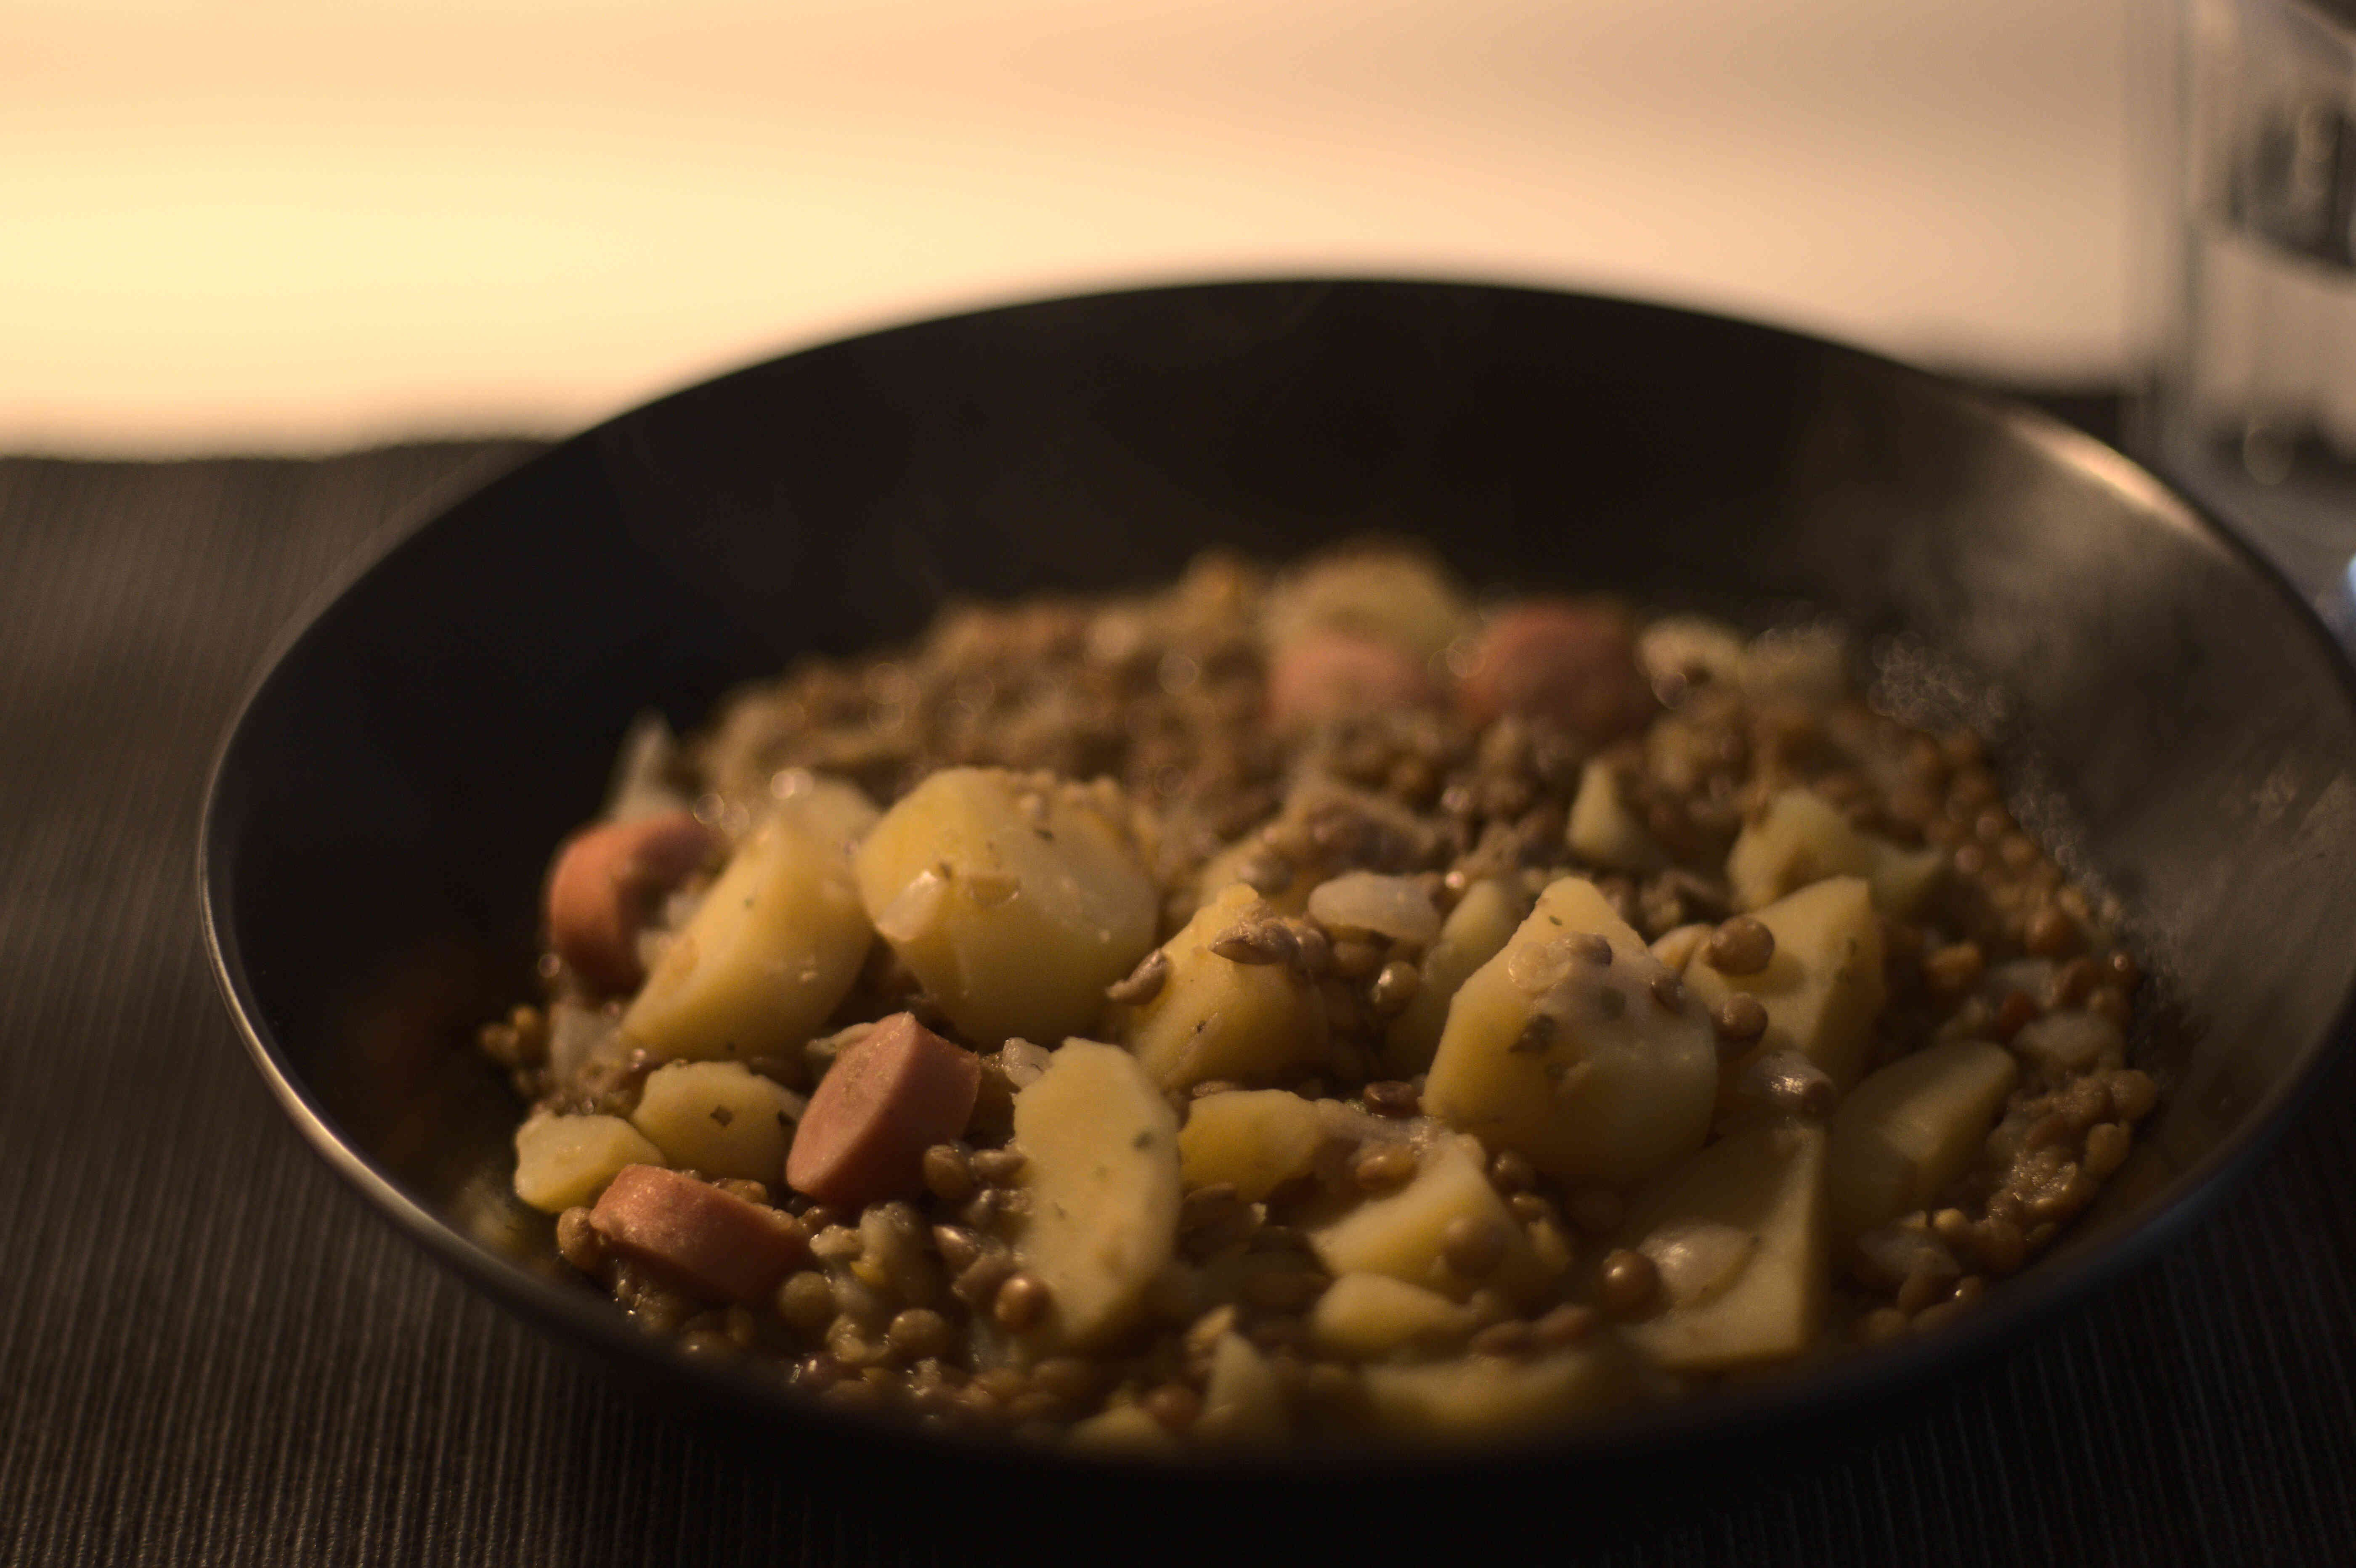
\includegraphics[height = 5cm]{media/linseneintopf.jpg}	\\
									&	\\
			\textbf{Beschreibung}	&	Wer hätte meinen können, dass ich mal einen Linseneintopf gern mögen würde?\\
									&	\\
			\begin{tabular}[t]{rr}
				\textbf{Zutaten}	\\
				Für 2 kg 			\\
				Für 6 Portionen	\\
			\end{tabular}			&	\begin{tabular}[t]{llll}
											1 kg & Kartoffeln \\
											4 	 & Möhren \\
											4 & Zwiebeln \\
											250 g & Linsen \\
											1,5 L & Gemüsebrühe \\
											200 g & Wiener Würstchen \\
											2 EL & Essig \\
											2 TL & Senf \\
											Salz, Pfeffer \\
											Petersilie \\
											Bratöl
										\end{tabular}	\\
									&	\\
			\textbf{Variationen}	&	\begin{itemize}[nosep]
											\item ...
										\end{itemize}	\\
									&	\\	
			\textbf{Passendes}		&	\begin{itemize}[nosep]
											\item Brot
										\end{itemize}	\\
									&	\\	
			% für zweiseitiges Rezept entkommentieren!
			\end{tabularx}
			\newpage
			\begin{tabularx}{\textwidth}{r|L}						
									
			\begin{tabular}[t]{rr}
				\textbf{Zubereitung}	\\
				Arbeitszeit: 1h	\\
				Garzeit: 30 min	\\
			\end{tabular}			&	\begin{enumerate}[nosep]
											\item Schäle und schneide die Kartoffeln, Zwiebeln und Möhren.
											\item Röste die Zwiebeln mit dem Bratöl in einem großen Topf an.
											\item Gib das Gemüse und die Brühe hinzu.
											\item Würze mit Pfeffer, Salz, Essig und Senf.
											\item Lasse alles 25-30 min kochen.
											\item Schneide die Wiener Würstchen in Scheiben und gib sie hinzu.
										\end{enumerate}	\\
		\end{tabularx}
		\newpage

		% Kartoffelpuffer

		\section{Kartoffelpuffer}	\label{kartoffelpuffer}

		\begin{tabularx}{\textwidth}{r|L}
									& 	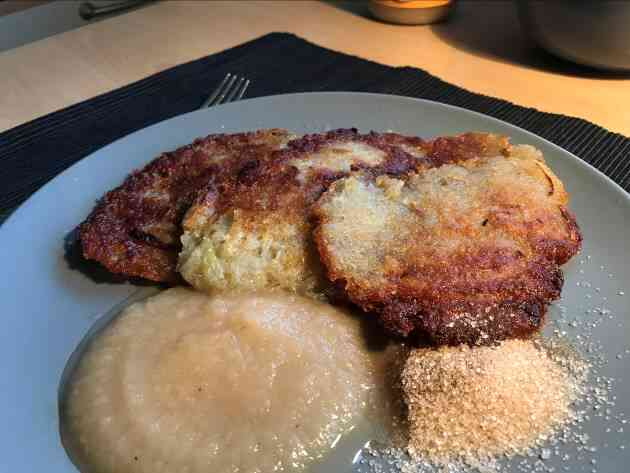
\includegraphics[height = 5cm]{media/kartoffelpuffer.jpg}	\\
									&	\\
			\textbf{Beschreibung}	&	Diese knusprigen Weise Kartoffeln zu Verarbeiten erinnert mich stets an den Kieler Weihnachtsmarkt. So nervig aufwenig in der Herstellung, wie auch unglaublich lecker!\\
									&	\\
			\begin{tabular}[t]{rr}
				\textbf{Zutaten}	\\
				Für 1.2 kg 			\\
				Für 4-6 Portionen	\\
			\end{tabular}			&	\begin{tabular}[t]{llll}
											1 kg & Kartoffeln, Zucchini \\
											3 & Zwiebeln, gewürfelt	\\
											1 EL & Mehl/Stärke \\
											Salz, Pfeffer \\
											viel hoch erhitzbares Öl! \\							
										\end{tabular}	\\
			%						&	\\
			%\textbf{Variationen}	&	\begin{itemize}[nosep]
			%								\item ...
			%							\end{itemize}	\\
									&	\\	
			\textbf{Passendes}		&	\begin{itemize}[nosep]
											\item Kräuterquark
											\item Apfelmus
											\item Zimt \& Zucker
										\end{itemize}	\\
									%&	\\	
			% für zweiseitiges Rezept entkommentieren!
		\end{tabularx}
		\newpage
		\begin{tabularx}{\textwidth}{r|L}	


			\begin{tabular}[t]{rr}
				\textbf{Zubereitung}	\\
				Vorbereitungszeit: 30-45 min	\\
				Garzeit: 5 min pro Stück		\\
			\end{tabular}			&	\begin{enumerate}[nosep]
											\item Schäle und reibe die Kartoffel (einfach gesagt, mühsam gemacht!)
											\item Drücke die Flüssigkeit aus den Kartoffeln in ein Gefäß und lasse es stehen, bis sich die Stärke absetzt und diese verwendet werden kann!
											\item Schneide die Zwiebeln in Würfel, gib sie mit dem Mehl zu den Kartoffeln und verrühre alles.
											\item Gib in eine Pfanne fingerdick hoch erhitzbares Öl hinein und führe den Holzstab-Test durch, bis es heiß genug ist.
											\item Nimm zwei Esslöffel der Kartoffeln und gib sie in das heiße Fett um einen Kartoffelpuffer zu machen. Nutze den Platz in der Pfanne gut!
											\item Lasse den Rand braun, aber nicht zu dunkel werden und wende den Puffer dann.
											\item Zuletzt lasse ihn in einer Schüssel etwas abkühlen, bevor er auf den Tisch kommt. 
										\end{enumerate}	\\
		\end{tabularx}
		\newpage

		\section{Indische Gerichte}

			% Curry

			\subsection{Aloo Masala (Kartoffel-Curry)}	\label{aloo_masala}

			\begin{tabularx}{\textwidth}{r|L}
										& 	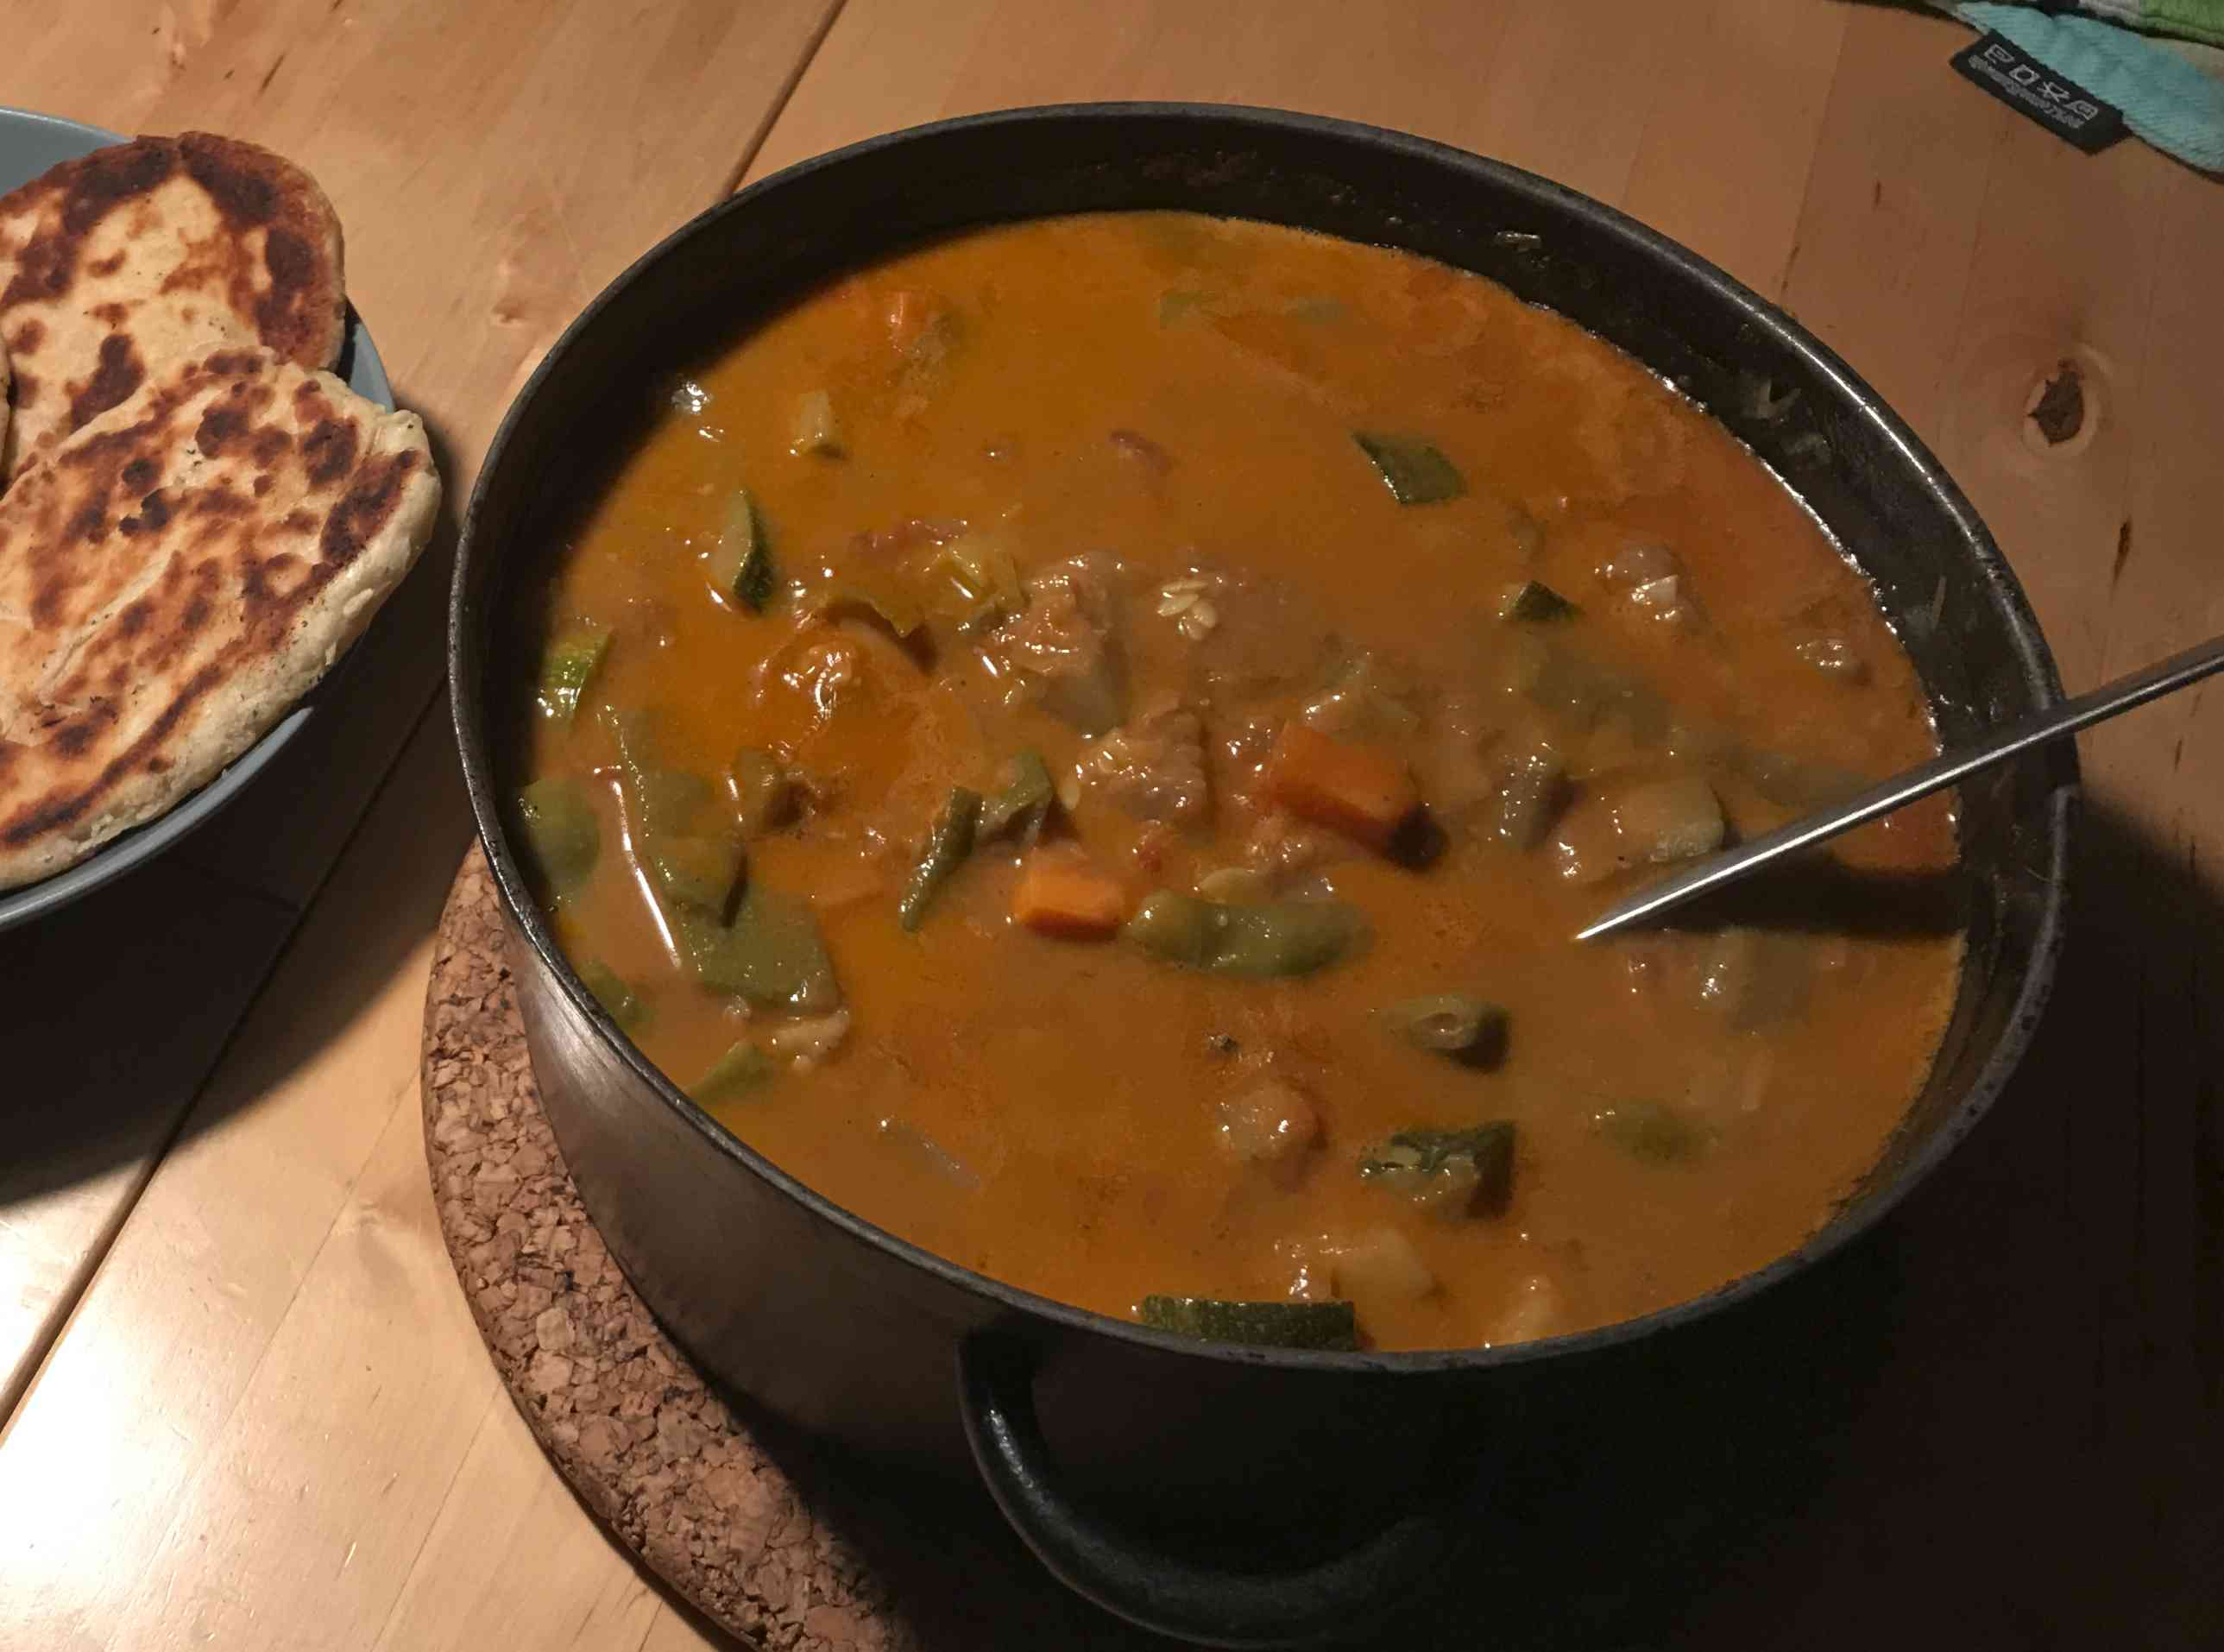
\includegraphics[height = 5cm]{media/aloo_masala.JPG}	\\
										&	\\
				\textbf{Beschreibung}	&	Ein guter Einstiege in die würzige indische Küche, mit dem alle Art von Gemüse zubereitet werden kann.\\
										&	\\
				\begin{tabular}[t]{rr}
					\textbf{Zutaten}	\\
					Für 1200 g 			\\
					Für 4 Portionen	\\
				\end{tabular}			&	\begin{tabular}[t]{llll}
												600 g (geht auch mehr) & Gemüse (Kartoffeln, Karotten \\ 
														& Zucchini, Aubergine, Kichererbsen, \\ 
														& Brokkoli, Lauch, Bohnen) \\
												3 große & Zwiebeln \\
												3 große oder 1 Dose & passierte Tomaten/frische Tomaten \\
												400 ml & Kokosmilch \\
												\\
												2 EL & Garam Masala \\
												1/2 TL & Chilipulver oder 1 Chilischote\\
												5 g Salz \\
												\\
												1 kleinen Zweig & Ingwer, geschält und geschnitten\\
												1 Zehe & Knoblauch \\
												alternativ 1 EL & Ginger-Garlic-Paste \\
												1 TL & Limettensaft \\
											\end{tabular}	\\
										&	\\
				\textbf{Variationen}	&	\begin{itemize}[nosep]
												\item mit Honig
												\item mit Erdnussbutter
												\item mit Hühnerfleisch
											\end{itemize}	\\

				\textbf{Passendes}		&	\begin{itemize}[nosep]
												\item Basmatireis
												\item Naan-Fladenbrot
											\end{itemize}	\\
				% für zweiseitiges Rezept entkommentieren!
			\end{tabularx}
			\newpage
			\begin{tabularx}{\textwidth}{r|L}	


				\begin{tabular}[t]{rr}
					\textbf{Zubereitung}	\\
					Arbeitszeit: 30 min \\ 
					schnippeln dauert...	\\
					Kochzeit: 20-30 min \\
					Gesamtzeit:	1h 		\\
				\end{tabular}			&	\begin{enumerate}[nosep]
												\item Schwitze die Zwiebeln mit Sonnenblumenöl an.
												\item Gib die Tomaten hinzu und lasse die Flüssigkeit etwas verkochen.
												\item Nun gib Garam Masala, Ginger-Garlic-Paste und die Chili hinzu und vermische alles gut.
												\item Schmecke die Würzung mit etwas Salz ab, sodass eine sehr intensive Grundlage für das Curry gegeben ist.
												\item Füge das Gemüse und die Kokosmilch hinzu und lasse alles köcheln, bis das Gemüse die gewünschte Konsistenz erreicht hat. Falls nötig kann zu Anfang so viel Wasser hinzugegeben werden um das Gemüse gerade zu bedecken. Zum Ende hin kann mit offenem Deckel gekocht werden um das Curry anzudicken .
											\end{enumerate}	\\
			\end{tabularx}
			\newpage

			% pav bhaji

			\subsection{Pav Bhaji}	\label{pav_bhaji}

			\begin{tabularx}{\textwidth}{r|L}
				%						& 	\includegraphics[height = 5cm]{media/vorlage.jpg}	\\
				%						&	\\
				\textbf{Beschreibung}	&	Ein Street-Food aus Indien, welches als sehr nährstoffreiches schnelles Essen für Textil-Arbeiter entwickelt wurde. Gesprochen "Pao bhatji"!\\
										&	\\
				\begin{tabular}[t]{rr}
					\textbf{Zutaten}	\\
					Für 800 g 			\\
					Für 4 Portionen	\\
				\end{tabular}			&	\begin{tabular}[t]{llll}
												1/2 kg & Kartoffeln \\
												2 große & Zwiebeln \\
												3 große oder 1 Dose & Tomaten \\
												100 g & Stangenbohnen/Erbsen \\
												50 g & Butter \\ 
												Salz, Pfeffer \\
												Pav Bhaji Masala \\

											\end{tabular}	\\
										&	\\
				\textbf{Variationen}	&	\begin{itemize}[nosep]
												\item ...
											\end{itemize}	\\
										&	\\	
				\textbf{Passendes}		&	\begin{itemize}[nosep]
												\item Helles Brot (am besten Pav)
											\end{itemize}	\\
										&	\\	
				\begin{tabular}[t]{rr}
					\textbf{Zubereitung}	\\
					Vorbereitungszeit: 20 min	\\
					Garzeit:	30-60 min		\\
				\end{tabular}			&	\begin{enumerate}[nosep]
												\item Schneide das Gemüse in kleine Stücke.
												\item Brate die Zwiebeln glasig an, gib den Knoblauch und die Tomaten hinzu und koche alles etwas ein.
												\item Füge das restliche Gemüse hinzu und dünste es mit Deckel bis es sehr weich ist.
												\item Zerstampfe oder püriere alles.
												\item Gib die Butter hinzu, würze alles mit Salz und Pav Bhaji Masala bis der gewünschte Geschmack erreicht ist.
											\end{enumerate}	\\
			\end{tabularx}
			\newpage

%----------------------------------<Gewürzmischungen>--------------------------------------

\chapter{Gewürzmischungen}

\newpage

	% Garam Masala

	\section{Garam Masala}	\label{garam_masala}

	\begin{tabularx}{\textwidth}{r|L}
		%						& 	\includegraphics[height = 5cm]{media/vorlage.jpg}	\\
		%						&	\\
		\textbf{Beschreibung}	&	Die Gewürzmischung welche die indischen Currys weltberühmt machte.\\
								&	\\
		\begin{tabular}[t]{rr}
			\textbf{Zutaten}	\\
			Für ... g 			\\
			Für ... Portionen	\\
		\end{tabular}			&	\begin{tabular}[t]{llll}	
										2 EL & Koriander \\
										1 EL & Piment \\
										1 EL & Kreuzkümmel/Cumin \\
										1 EL & Paprikapulver \\
										1/2 EL & Zimt \\
										1/2 TL & Chilipulver \\
										1/2 TL & Nelken \\
										1/2 TL & Anis \\
										1/2 TL & schwarzer Pfeffer \\					
									\end{tabular}	\\
								&	\\
		\textbf{Variationen}	&  \begin{itemize}[nosep]
										\item für gelbes Masala füge 1 EL Kurkuma hinzu
 									\end{itemize}\\
		\begin{tabular}[t]{rr}
			\textbf{Zubereitung}	\\
			Vorbereitungszeit: 15 min	\\
			Garzeit:	5 min		\\
		\end{tabular}			&	\begin{enumerate}[nosep]
										\item Röste die genannten Zutaten in einer Pfanne an und mahle sie anschließend zu einem Pulver.
									\end{enumerate}	\\
	\end{tabularx}
	\newpage

	% Pav Bhaji Masala

	\section{Pav Bhaji Masala}	\label{pav_bhaji_masala}

	\begin{tabularx}{\textwidth}{r|L}
		%						& 	\includegraphics[height = 5cm]{media/vorlage.jpg}	\\
		%						&	\\
		\textbf{Beschreibung}	&	Die Gewürzmischung hinter dem indischen Street-Food-Klassiker.\\
								&	\\
		\begin{tabular}[t]{rr}
			\textbf{Zutaten}	\\
			Für ... g 			\\
			Für ... Portionen	\\
		\end{tabular}			&	\begin{tabular}[t]{llll}
										2 TL & Koriander \\
										1 TL & grüner Kardamom \\
										1 TL & schwarzer Kardamom \\
										1 TL & Cumin \\
										1 TL & Pfefferkörner \\
										1/2 TL & Chilipulver \\
										1/2 TL & Zimt \\
										1 TL & Nelken \\
										1/2 TL & Anis \\
										1/2 TL & Muskat \\
										1 TL & Paprika 	\\
										? 1/2 TL & Fenchel ?						
									\end{tabular}	\\
								&	\\	
		\begin{tabular}[t]{rr}
			\textbf{Zubereitung}	\\
			Vorbereitungszeit: 15 min	\\
			Garzeit:	5 min		\\
		\end{tabular}			&	\begin{enumerate}[nosep]
										\item Röste die genannten Zutaten in einer Pfanne an und mahle sie anschließend zu einem Pulver.
									\end{enumerate}	\\
	\end{tabularx}
	\newpage


%----------------------------------<Süßspeisen>--------------------------------------

\chapter{Süßspeisen}

\newpage

		% Pfannkuchen

		\section{Pfannkuchen}	\label{pfannkuchen}

		\begin{tabularx}{\textwidth}{r|L}
									& 	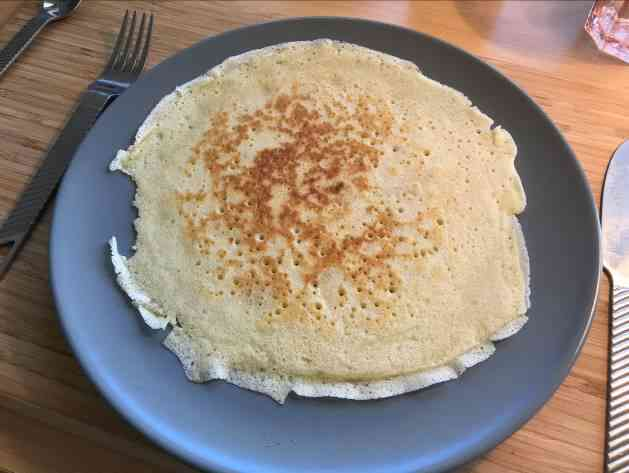
\includegraphics[height = 5cm]{media/pfannkuchen.jpg}	\\
									&	\\
			\textbf{Beschreibung}	&	Was gibt es schöneres als morgens mit einem frischen Pfannkuchenfrühstück in einen Sonntag zu starten?\\
									&	\\
			\begin{tabular}[t]{rr}
				\textbf{Zutaten}	\\
				Für 900 g 			\\
				Für 2 Portionen	\\
				Für 6-8 Pfannkuchen \\
			\end{tabular}			&	\begin{tabular}[t]{llll}
											300 g & Mehl \\
											400 ml & Milch \\
											2 & Eier \\
											40 g & Zucker \\
											30 g & Butter, Öl \\
											1 Prise & Salz \\
											1 TL & Backpulver \\								
										\end{tabular}	\\
									&	\\
			\textbf{Variationen}	&	\begin{itemize}[nosep]
											\item Käsepfannkuchen
											\item Pancakes
											\item Crêpe
											\item Spinatpfannkuchen (Spinat, Zwiebeln, Knoblauch, Frischkäse)
										\end{itemize}	\\
									&	\\	
			\textbf{Passendes}		&	\begin{itemize}[nosep]
											\item Ahornsirup, Marmelade, Schokocrème mit Banane, Zucker mit Zitronensaft
										\end{itemize}	\\
									&	\\	
		\end{tabularx}

		\begin{tabularx}{\textwidth}{r|L}
			\begin{tabular}[t]{rr}
				\textbf{Zubereitung}	\\
				Arbeitszeit: 15 + 30 min \\
				Gesamtzeit:	45 min		\\
			\end{tabular}			&	\begin{enumerate}[nosep]
											\item Vermische das Mehl mit dem Salz und einem Teil des Zucker in einer angemessen großen Schüssel.
											\item Trenne des Ei und schlage es mit dem übrigen Zucker zu Eischnee.
											\item Gib anfangs einen Teil der Milch zum Teig und verrühre alles möglichst homogen.
											\item Schütte den Rest der Milch hinzu und überprüfe, ob die gewünschte Konsistenz erreicht ist.
											\item Hebe den Eischnee per Hand mit einem Teigschaber oder Ähnlichem unter, sodass die Luft eingeschlossen bleibt.
											\item Lasse den Pfannkuchenteig für 30 min quellen, damit die Stärke im Mehl ein wenig Wasser aufnehmen kann.
											\item Überprüfe, dass der Teig tatsächlich zähflüssiger geworden ist und rühre ihn noch einmal durch.
											\item Heize eine angemessen große Pfanne vor und gib die Butter zum Schmelzen hinein.
											\item Rühre die Butter unter den Teig und bereite dich auf das Pfannkuchen-Backen vor.
											\item Stelle die Pfanne auf mittlere Hitze und eine halbe Kelle (~80 g) Teig pro Pfannkuchen in die Pfanne. Es sollte neben der Butter im Teig kein weiteres Fett benötigt werden.
											\item Möchte man dicke Pfannkuchen haben, kann man den Teig ohne Bewegen der Pfanne zerfließen lassen. Andernfalls schwenkt man die Pfanne oder verteilt den Teig mit einem Pfannenschaber.
											\item Wende den Pfannkuchen, wenn ordentlich Blasen durch das Backpulver entstanden sind und die Unterseite angemessen braun ist.
											\item Backe nun die andere Seite nur kurz, da der Teig schon gut durchgebacken ist und nur noch wenig Zeit benötigt.
											\item Lege den fertigen Pfannkuchen zwischen zwei Teller mit den Anderen, um sie schön saftig und weich zu haben. Will man eher einen knusprigen Pfannkuchen, lässt man ihn an der Luft abkühlen.
										\end{enumerate}	\\
		\end{tabularx}

		\begin{figure}[h]
			\centering
			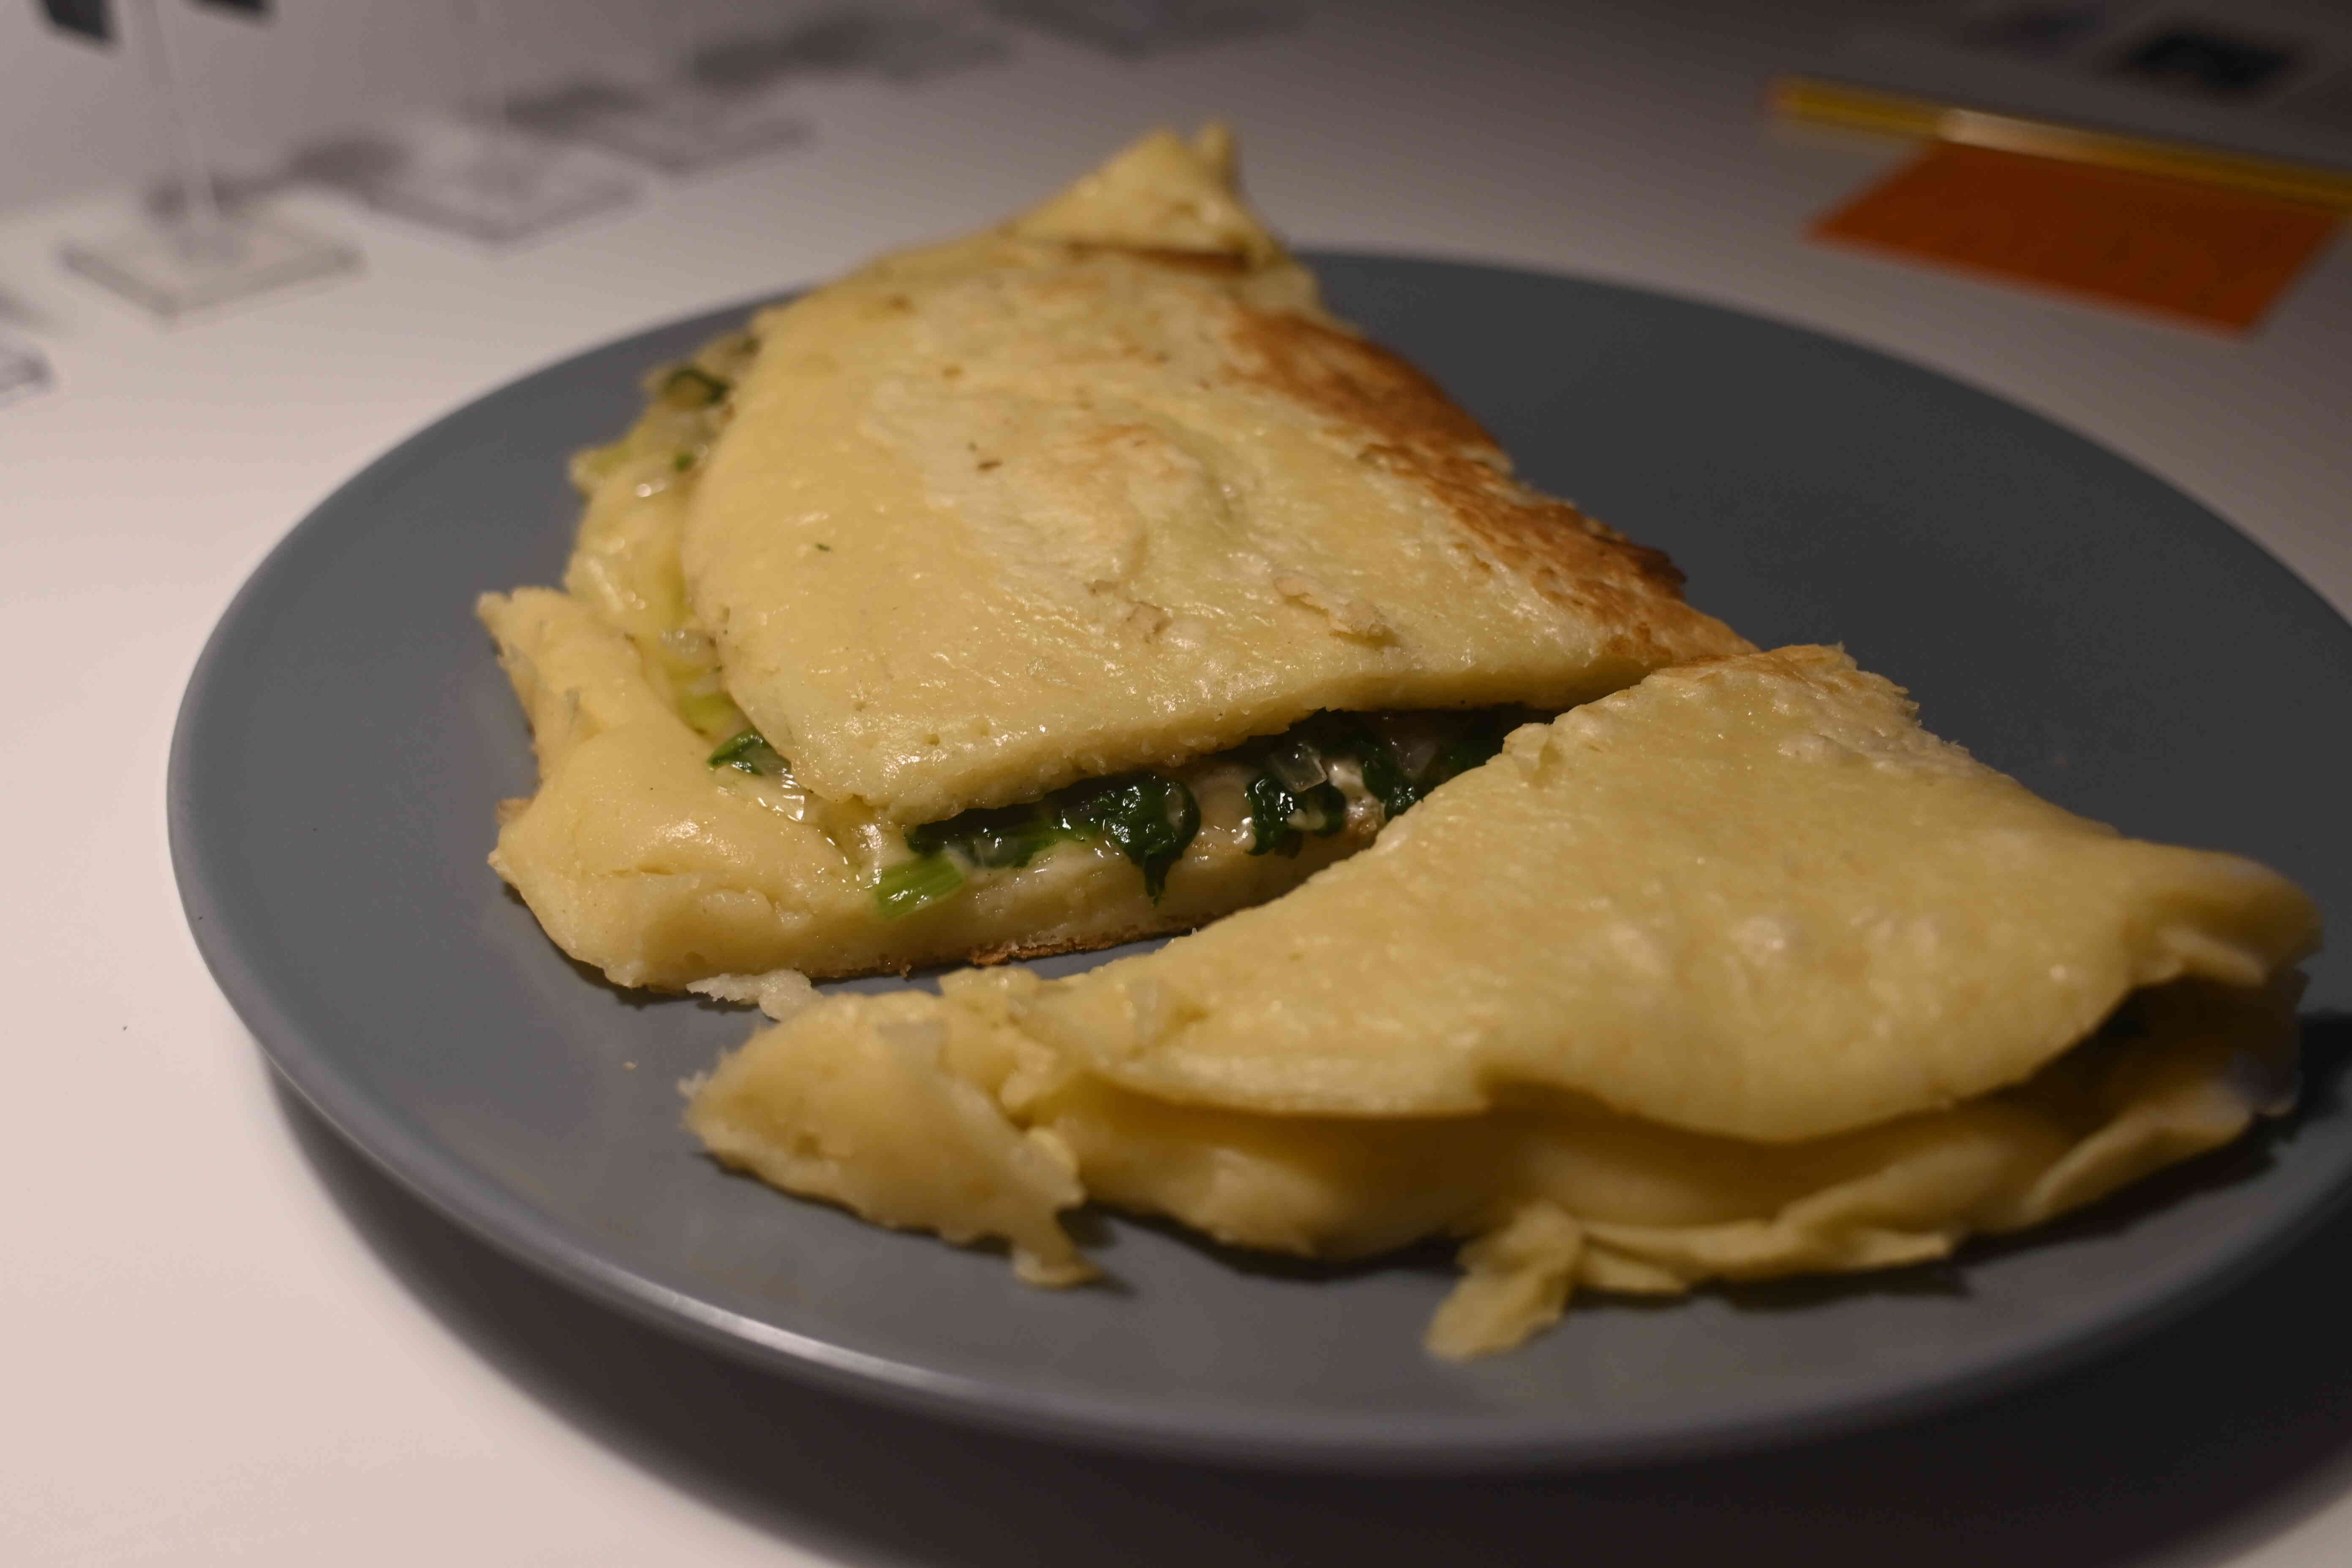
\includegraphics[width = 0.6\textwidth]{media/spinat_pfannkuchen.JPG}
			\caption{Spinatpfannkuchen mit Spinat aus dem Ellener Hof Gemeinschaftsgarten!}
		\end{figure}

		\newpage

		% Dampfnudeln

		\section{Dampfnudeln}	\label{dampfnudeln}

		\begin{tabularx}{\textwidth}{r|L}
									& 	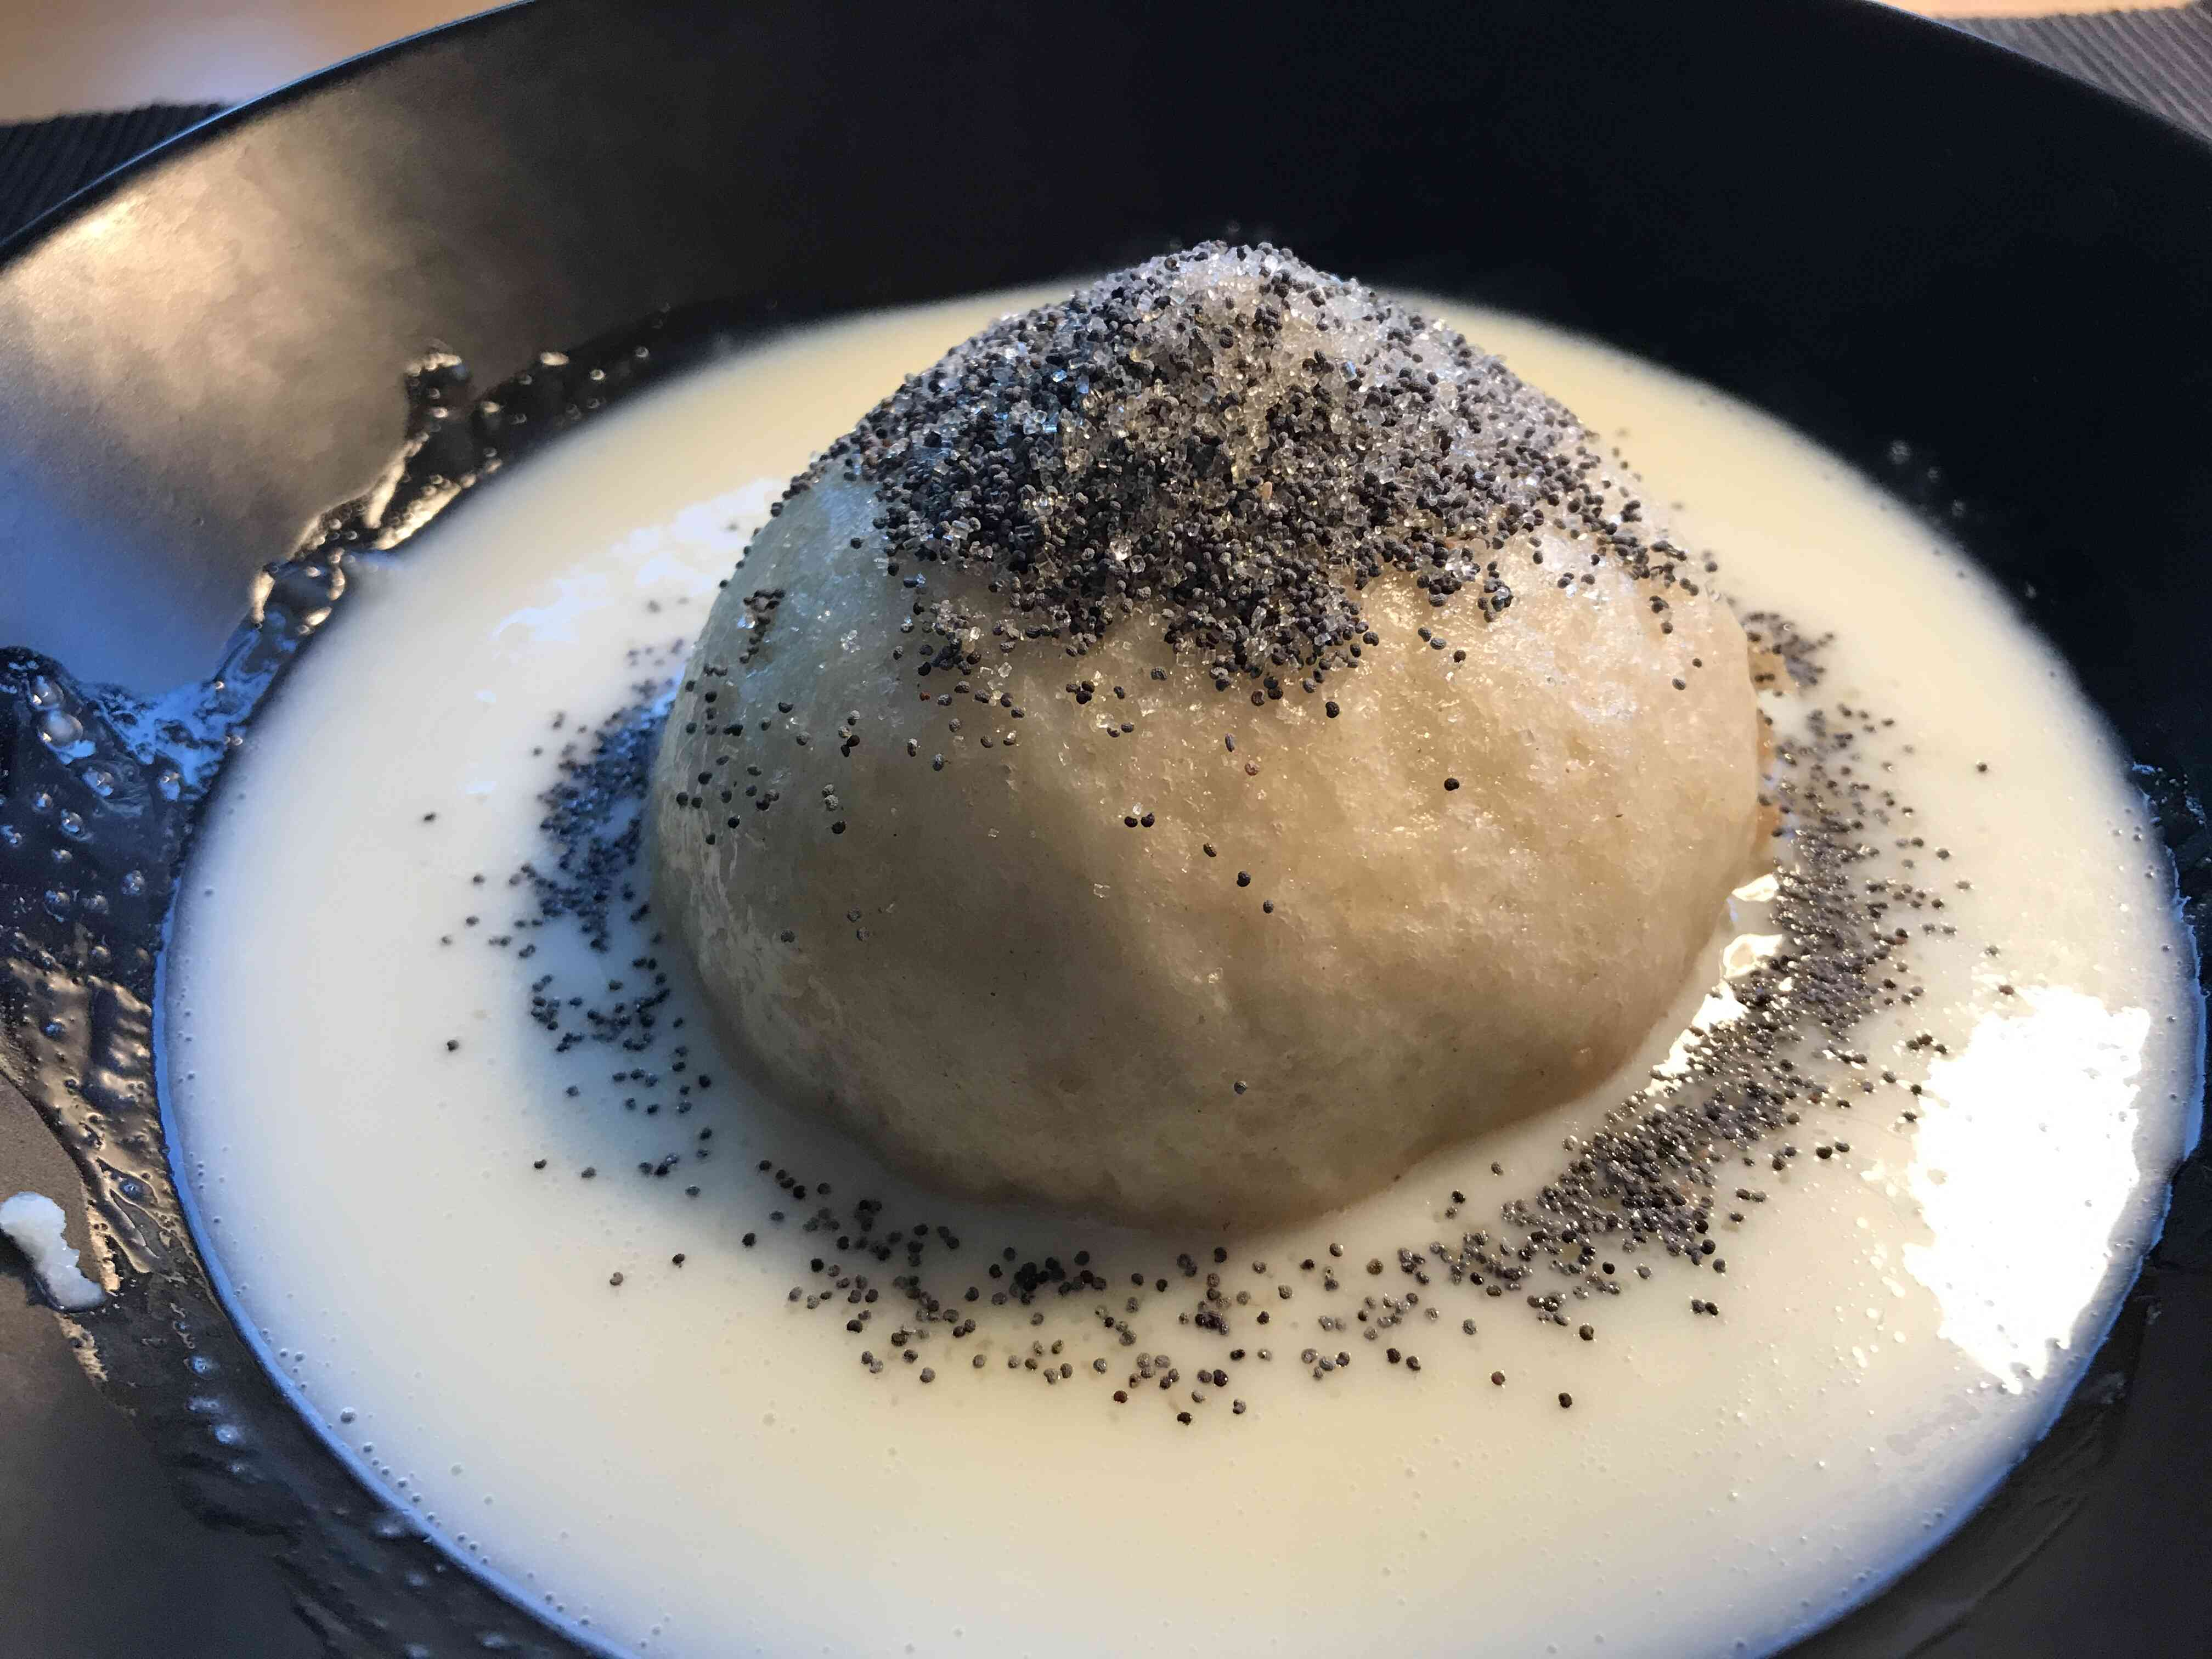
\includegraphics[height = 5cm]{media/dampfnudel.jpg}	\\
									&	\\
			\textbf{Beschreibung}	&	In Erinnerung an den Kieler Weihnachtsmarkt, auf dem ich stets die Dampfnudeln mit Vanillesoße und Mohnzucker gegessen habe.\\
									&	\\
			\begin{tabular}[t]{rr}
				\textbf{Zutaten}	\\
				Für 680 g 			\\
				Für 4 Portionen	\\
			\end{tabular}			&	\begin{tabular}[t]{llll}
											Dampfnudelteig: \\
											\begin{tabular}{lll}
												400 g & Weizenmehl, 550er \\
												200 g & Milch \\
												15 g & Zucker \\
												4 g & Salz \\
												60 g & Butter \\
												1 g & Trockenhefe \\
											\end{tabular} \\
											\\
											Füllung: \\
											\begin{tabular}{ll}
												4 x 1 EL & Pflaumenmuß, Marmelade \\
											\end{tabular} \\
											\\
											Zum Kochen in reichlich Wasser: \\
											\begin{tabular}{lll}
												500 ml & Wasser \\
												5-7 g & Salz \\
											\end{tabular} \\
											ODER zum Dämpfen bis das Wasser verkocht: \\
											\begin{tabular}{lll}
												300 ml & Wasser \\
												3 EL & Öl \\
												3 g & Salz \\
											\end{tabular} \\
										\end{tabular}	\\
									&	\\
			\textbf{Variationen}	&	\begin{itemize}[nosep]
											\item ...
										\end{itemize}	\\
									&	\\	
			\textbf{Passendes}		&	\begin{itemize}[nosep]
											\item Vanillesoße
											\item Mohnzucker
										\end{itemize}	\\
									&	\\	
									
		\end{tabularx}

		\begin{tabularx}{\textwidth}{r|L}
			\begin{tabular}[t]{rr}
				\textbf{Zubereitung}	\\
				Arbeitszeit: 30 min	\\
				Gehzeit: 12-24 h \\
				Kochzeit: 20 min \\
			\end{tabular}			&	\begin{enumerate}[nosep]
											\item Löse die Hefe in der Flüssigkeit in einer angemessen großen Schüssel auf.
											\item Gib das Mehl, die Butter, den Zucker und das Salz hinzu und verrühre kurz alles homogen.
											\item Knete nun den Teig für 10 min ordentlich, sodass sich das Gluten gut bilden kann.
											\item Lasse den Teig 20-24 h bei Zimmertemperatur gehen.
											\item Bringe den Teig, mit möglichst wenig Mehleinsatz, nun wieder unter Spannung, fülle ihn eventuell und forme eine Kugel.
											\item Lasse den Teigling 1-3 h abgedeckt ruhen, sodass er ordentlich an Größe gewinnt und nicht austrocknet.
											\item Gib das Wasser, das Öl und das Salz in einen großen Topf mit Deckel und bringe es zum Kochen.
											\item Gibt die Teiglinge hinzu, regle die Hitze herunter und lasse sie für 20 min bei geschlossenem Deckel garen.
										\end{enumerate}	\\
		\end{tabularx}
		\newpage

		% Vanillesoße

		\section{Vanille-Soße und -Pudding}	\label{vanillesosse}

		\begin{tabularx}{\textwidth}{r|L}
			%						& 	\includegraphics[height = 5cm]{media/vorlage.jpg}	\\
			%						&	\\
			\textbf{Beschreibung}	&	Eine wichtige Dessertsoße oder mit mehr Stärke auch ein Pudding. \\
									&	\\
			\begin{tabular}[t]{rr}
				\textbf{Zutaten}	\\
				Für 250 g 			\\
				Für 1 Portionen	\\
			\end{tabular}			&	\begin{tabular}[t]{llll}
											200 g & Milch \\
											25 g & Zucker \\
											für Soße: 12 g \\
											für Pudding: 24 g & Stärke \\
											Vanille \\
											Salz \\								
										\end{tabular}	\\
									&	\\
			\textbf{Variationen}	&	\begin{itemize}[nosep]
											\item Schokopudding mit 10g Kakaopulver
										\end{itemize}	\\
									&	\\	
			\textbf{Passendes}		&	\begin{itemize}[nosep]
											\item Dampfnudeln (Rezept \ref{dampfnudeln})
										\end{itemize}	\\
									&	\\	
			\begin{tabular}[t]{rr}
				\textbf{Zubereitung}	\\
			\end{tabular}			&	\begin{enumerate}[nosep]
											\item Löse die Stärke, den Zucker in einem Teil der kalten Milch und gib die Vanille hinzu.
											\item Bringe die Milch zum Kochen und rühre anschließend die Pudding-Mischung ein.
											\item Lasse alles ein paar Minuten unter rühren ordentlich kochen und gib es in ein anderes Gefäß zum Abkühlen.
											\item Sobald der Pudding abkühlt sollte die gewünschte Konsistenz erreicht werden.
										\end{enumerate}	\\
		\end{tabularx}
		\newpage


		% Waffeln

		\section{Waffeln}	\label{waffeln}

		\begin{tabularx}{\textwidth}{r|L}
			%						& 	\includegraphics[height = 5cm]{media/vorlage.jpg}	\\
			%						&	\\
			\textbf{Beschreibung}	&	Ein leckeres Sonntagsessen, wobei die Frequenz $f$ mit der man Waffeln bekommt antiproportional mit der Teilnehmeranzahl $n$ abnimmt! Hierbei ist $T_w$ die Zeit zur Fertigstellung einer Waffel: $$f = \frac{1}{nT_w}$$\\
									&	\\
			\begin{tabular}[t]{rr}
				\textbf{Zutaten}	\\
				Für 1 kg 			\\
				Für 10 Portionen und 3-5 Personen	\\
			\end{tabular}			&	\begin{tabular}[t]{llll}
											250 g & Weizenmehl, 550er \\
											1/4 L & Milch \\
											120 g & Butter \\
											120 g & Zucker \\
											3 & Eier \\
											1/2 TL & Backpulver \\
										\end{tabular}	\\
									&	\\
			\textbf{Variationen}	&	\begin{itemize}[nosep]
											\item ...
										\end{itemize}	\\
									&	\\	
			\textbf{Passendes}		&	\begin{itemize}[nosep]
											\item Schlagsahne
											\item Kirschen
										\end{itemize}	\\
									&	\\	
			\begin{tabular}[t]{rr}
				\textbf{Zubereitung}	\\
				Arbeitszeit: 15 min	\\
				Garzeit pro Waffel: 2-3 min	\\
			\end{tabular}			&	\begin{enumerate}[nosep]
											\item Butter mit dem Zucker vermischen und Eier hinzugeben.
											\item Separat das Mehl mit dem Backpulver mischen und anschließend kurz in die Zucker-Butter-Ei-Masse einrühren.
											\item Lasse den Teig optimalerweise vor dem Backen mind. 30 min im Kühlschrank quellen für eine bessere Konsistenz.
											\item Heize das Waffeleisen ordentlich auf, gib etwas Butter auf die Backfläche und gib mit einer Kelle ca. 100g des Waffelteigs hinein.
											\item Backe 2-3 min für eine Waffel bis zum gewünschten Bräunungsgrad.
										\end{enumerate}	\\
		\end{tabularx}
		\newpage


		% Grießbrei

	\section{Grießbrei oder Grießpudding}	\label{grießbrei}
	\begin{tabularx}{\textwidth}{r|L}
								& 	\includegraphics[height = 5cm]{media/grießbrei.JPG}	\\
								&	\\
		\textbf{Beschreibung}	&	... \\
								&	\\
		\begin{tabular}[t]{rr}
			\textbf{Zutaten}	\\
			Für 250 g 			\\
			Für 1 Portionen	\\
		\end{tabular}			&	\begin{tabular}[t]{llll}
										200 g & Milch \\
										40 g / 2 EL & Hartweizengrieß \\
										10 g / 1,5 TL & Zucker \\
										10 g & Butter \\								
									\end{tabular}	\\
								&	\\
		\textbf{Variationen}	&	\begin{itemize}[nosep]
										\item Grießpudding mit erhöhen auf 80 g Grieß
									\end{itemize}	\\
								&	\\	
		\textbf{Passendes}		&	\begin{itemize}[nosep]
										\item Rosinen
										\item Butter
										\item Apfelmus
										\item Zimt \& Zucker
									\end{itemize}	\\
								&	\\	
		\begin{tabular}[t]{rr}
			\textbf{Zubereitung}	\\
			Arbeitszeit: 10 min
		\end{tabular}			&	\begin{enumerate}[nosep]
										\item Gib Milch mit dem Zucker in einen Topf und bringe sie zum Kochen.
										\item Füge nun den Grieß hinzu und rühre gut, während der Grießbrei deutlich andicken sollte.
										\item Nun kann der Brei von der Herdplatte genommen werden und muss nur noch für 5 min quellen gelassen werden. Dabei kann er schon in die Gefäße zum Servieren gegeben werden!
									\end{enumerate}	\\
	\end{tabularx}
	\newpage


	% Milchreis

 \section{Milchreis}	\label{milchreis}

 \begin{tabularx}{\textwidth}{r|L}
 	%						& 	\includegraphics[height = 5cm]{media/vorlage.jpg}	\\
 	%						&	\\
 	\textbf{Beschreibung}	&	Eine schöne Abwechlsung zu anderen Reiszubereitungen ist dieser Traum eines eden Kindes. \\
 							&	\\
 	\begin{tabular}[t]{rr}
 		\textbf{Zutaten}	\\
 		Für 270 g 			\\
 		Für 1 Portionen	\\
 	\end{tabular}			&	\begin{tabular}[t]{llll}
 									50 g & Rundkornreis \\
 									200 g & Milch (mit extra Sahne)	\\
 									10 g & Zucker 	\\
									1 Prise & Salz							
 								\end{tabular}	\\
 							&	\\
 	\textbf{Variationen}	&	\begin{itemize}[nosep]
 									\item ...
 								\end{itemize}	\\
 							&	\\	
 	\textbf{Passendes}		&	\begin{itemize}[nosep]
 									\item Zimt \& Zucker
 									\item Kirschen
 									\item Apfelmus
 								\end{itemize}	\\
 							&	\\	
 	\begin{tabular}[t]{rr}
 		\textbf{Zubereitung}	\\
 		Arbeitszeit: 1h	\\
 		Kochzeit: 40 min		\\
 	\end{tabular}			&	\begin{enumerate}[nosep]
 									\item Gib die Milch in einen Topf und löse den Zucker auf.
									\item Bringe die Milch zum Kochen und gib den Milchreis hinzu.
									\item Stelle die Platte auf die kleinste Flamme, rühre alle 10 min und lasse es insgesamt 40 min kochen.
									\item Überprüfe, ob die gewünschte Konsistenz erreicht ist und lasse ihn ein wenig abkühlen.
 								\end{enumerate}	\\
 \end{tabularx}
 \newpage

	

%----------------------------------<Snacks>--------------------------------------

\chapter{Snacks}

	% Karamell

	\section{Karamell}	\label{karamell}

	\begin{tabularx}{\textwidth}{r|L}
								& 	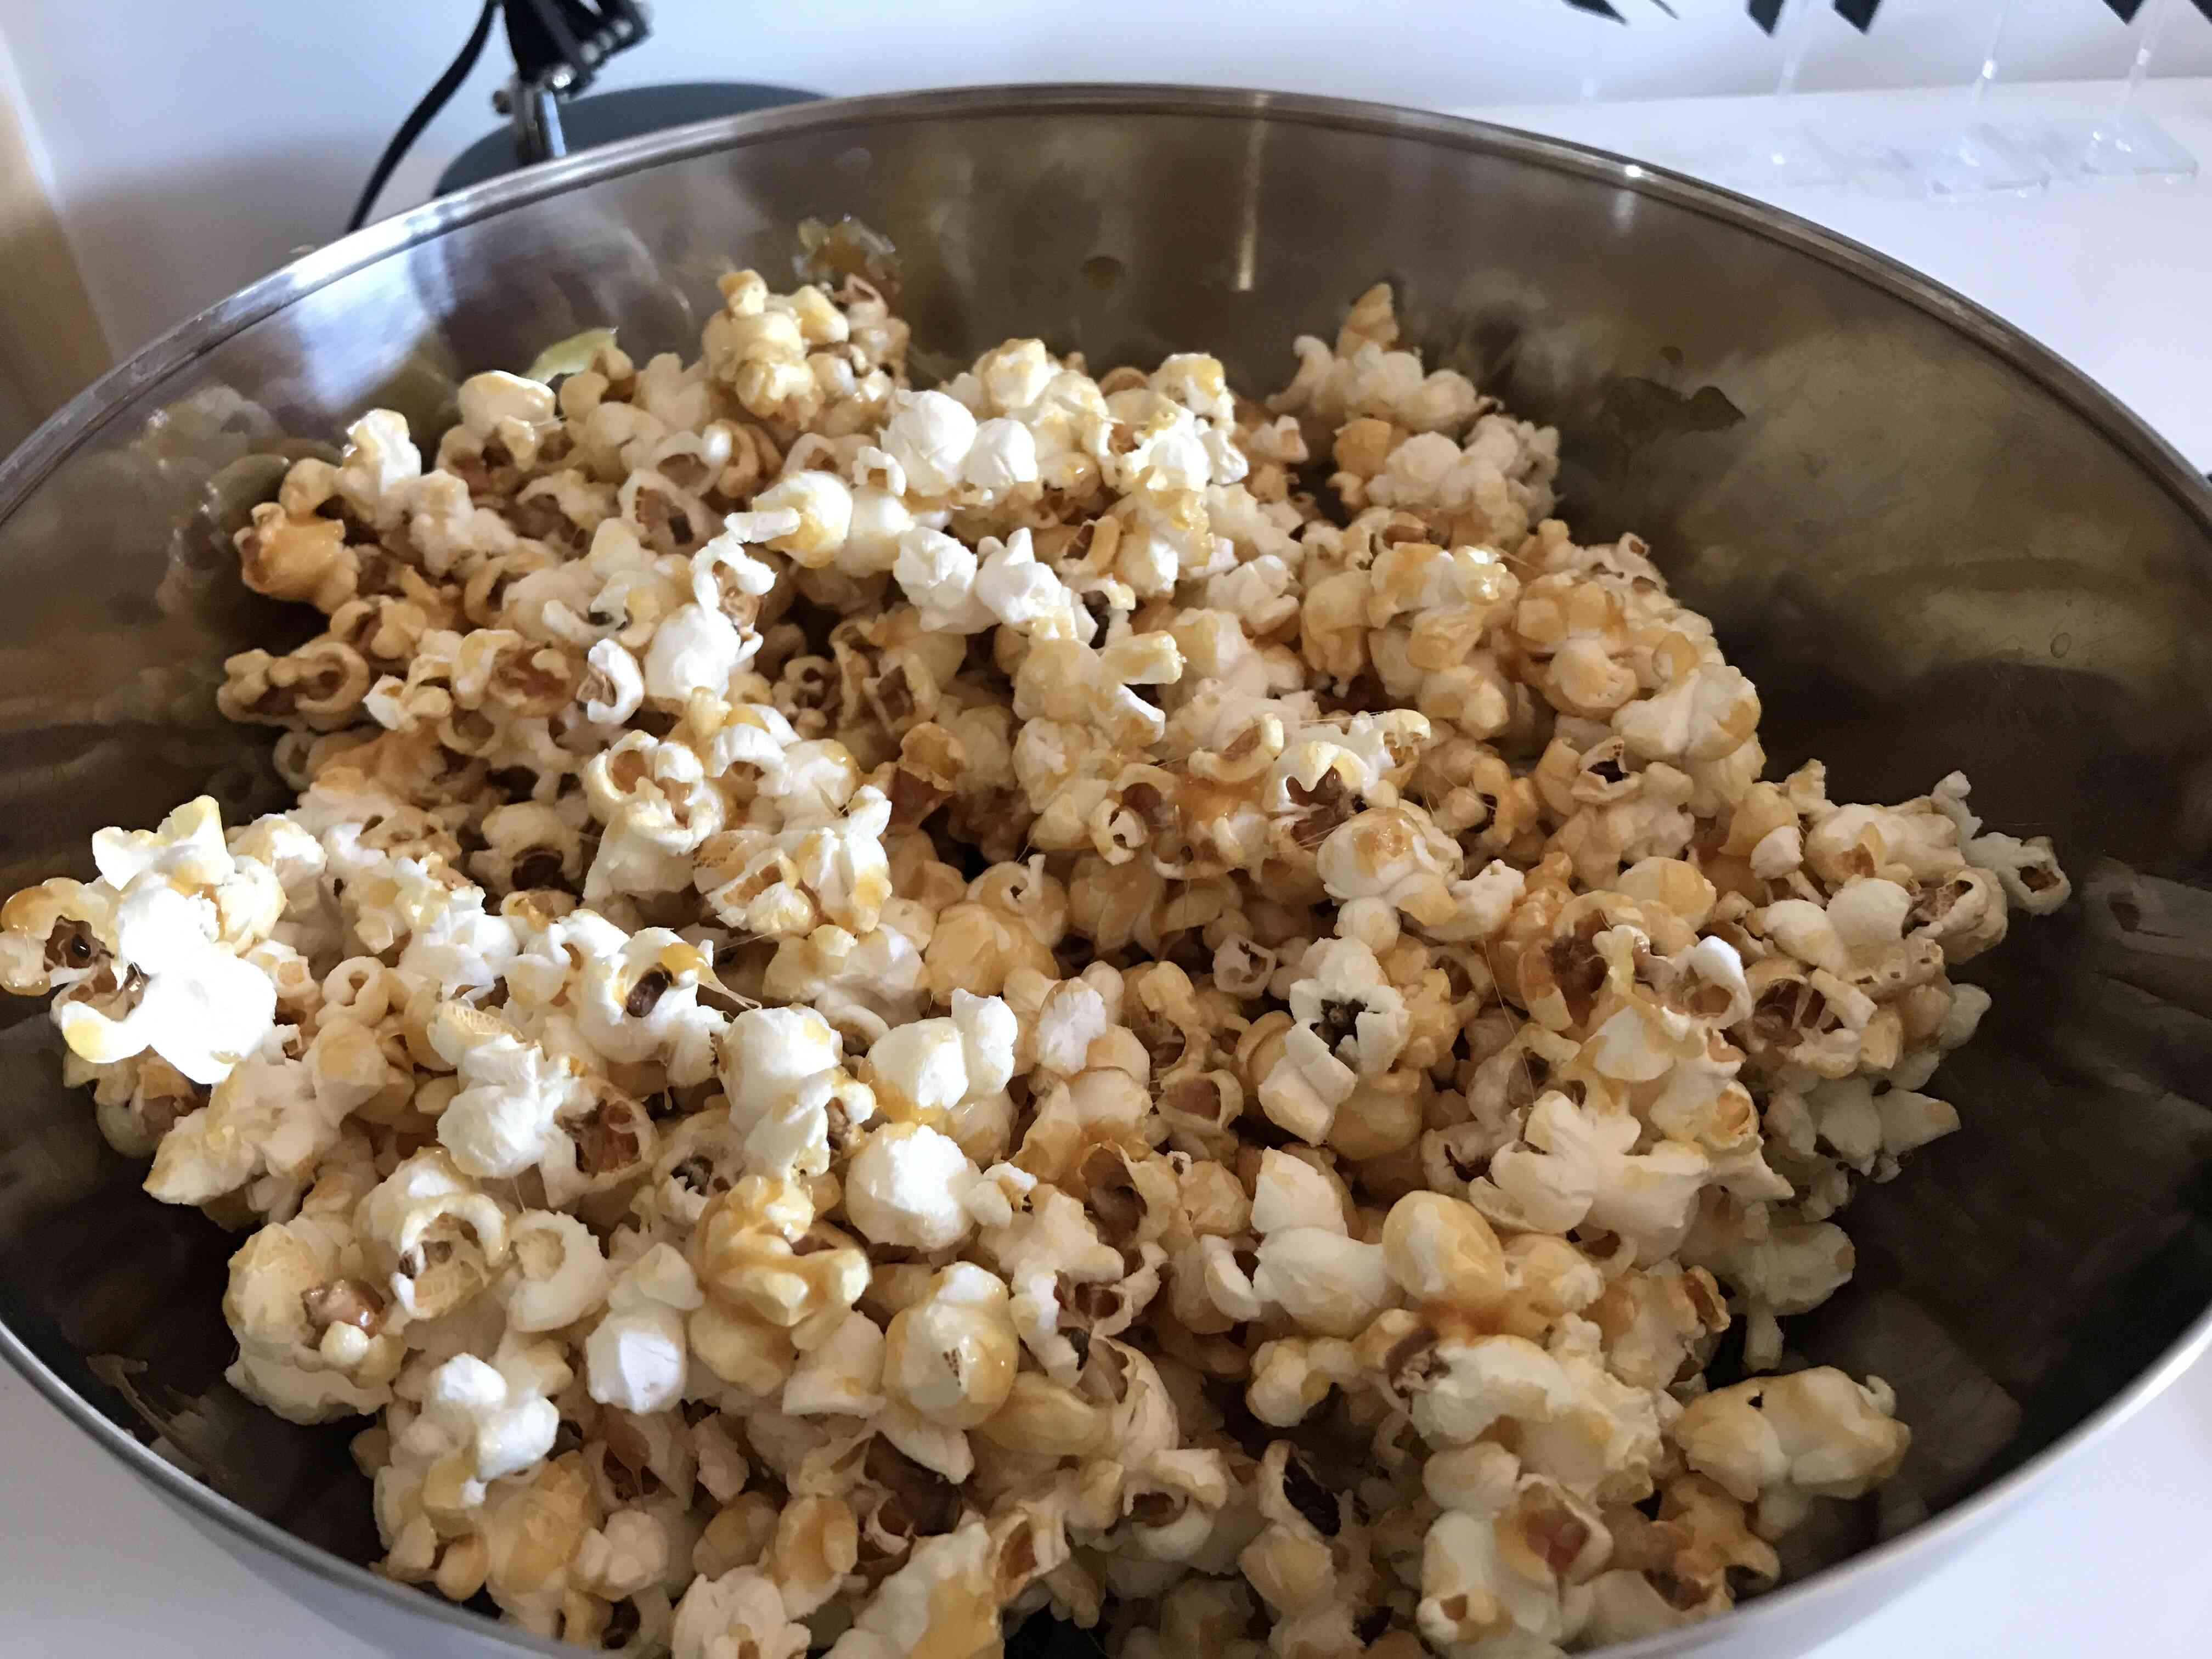
\includegraphics[height = 5cm]{media/popcorn.jpg}	\\
								&	\\
		\textbf{Beschreibung}	&	Wenn man nur Zucker und Butter zuhause hat, kann man immernoch Karamell herzustellen!\\
								&	\\
		\begin{tabular}[t]{rr}
			\textbf{Zutaten}	\\
			Für 110 g 			\\
			Für 4 Portionen	\\
		\end{tabular}			&	\begin{tabular}[t]{llll}
										100 g & Zucker &\\
										10 g & Butter & (Anteil nach gewünschter Karamell-Konsistenz \\ & & wählen!)\\	
										1 g & Salz & 							
									\end{tabular}	\\
								&	\\
		\textbf{Variationen}	&	\begin{itemize}[nosep]
										\item Karamellpopcorn
										\item Fudge (1:1 Zucker zu Butter)
										\item Zuckerwatte
										\item Creme Brulée
									\end{itemize}	\\
								&	\\	
		\textbf{Passendes}		&	\begin{itemize}[nosep]
										\item ...
									\end{itemize}	\\
								&	\\	
		\begin{tabular}[t]{rr}
			\textbf{Zubereitung}	\\
			Arbeitszeit: 20 min	\\
		\end{tabular}			&	\begin{enumerate}[nosep]
										\item Gib den Zucker in einen leicht zu spülenden Topf und erhitze ihn, bis er eine leichte Verfärbung sehen lässt.
										\item Ergänze den geschmolzenen Zucker mit der gewünschten Buttermenge und rühre alles gut um.
									\end{enumerate}	\\
	\end{tabularx}
	\newpage

	% Pizzabrötchen

	\section{Pizzabrötchen}	\label{pizzabroetchen}

	\begin{tabularx}{\textwidth}{r|L}
								& 	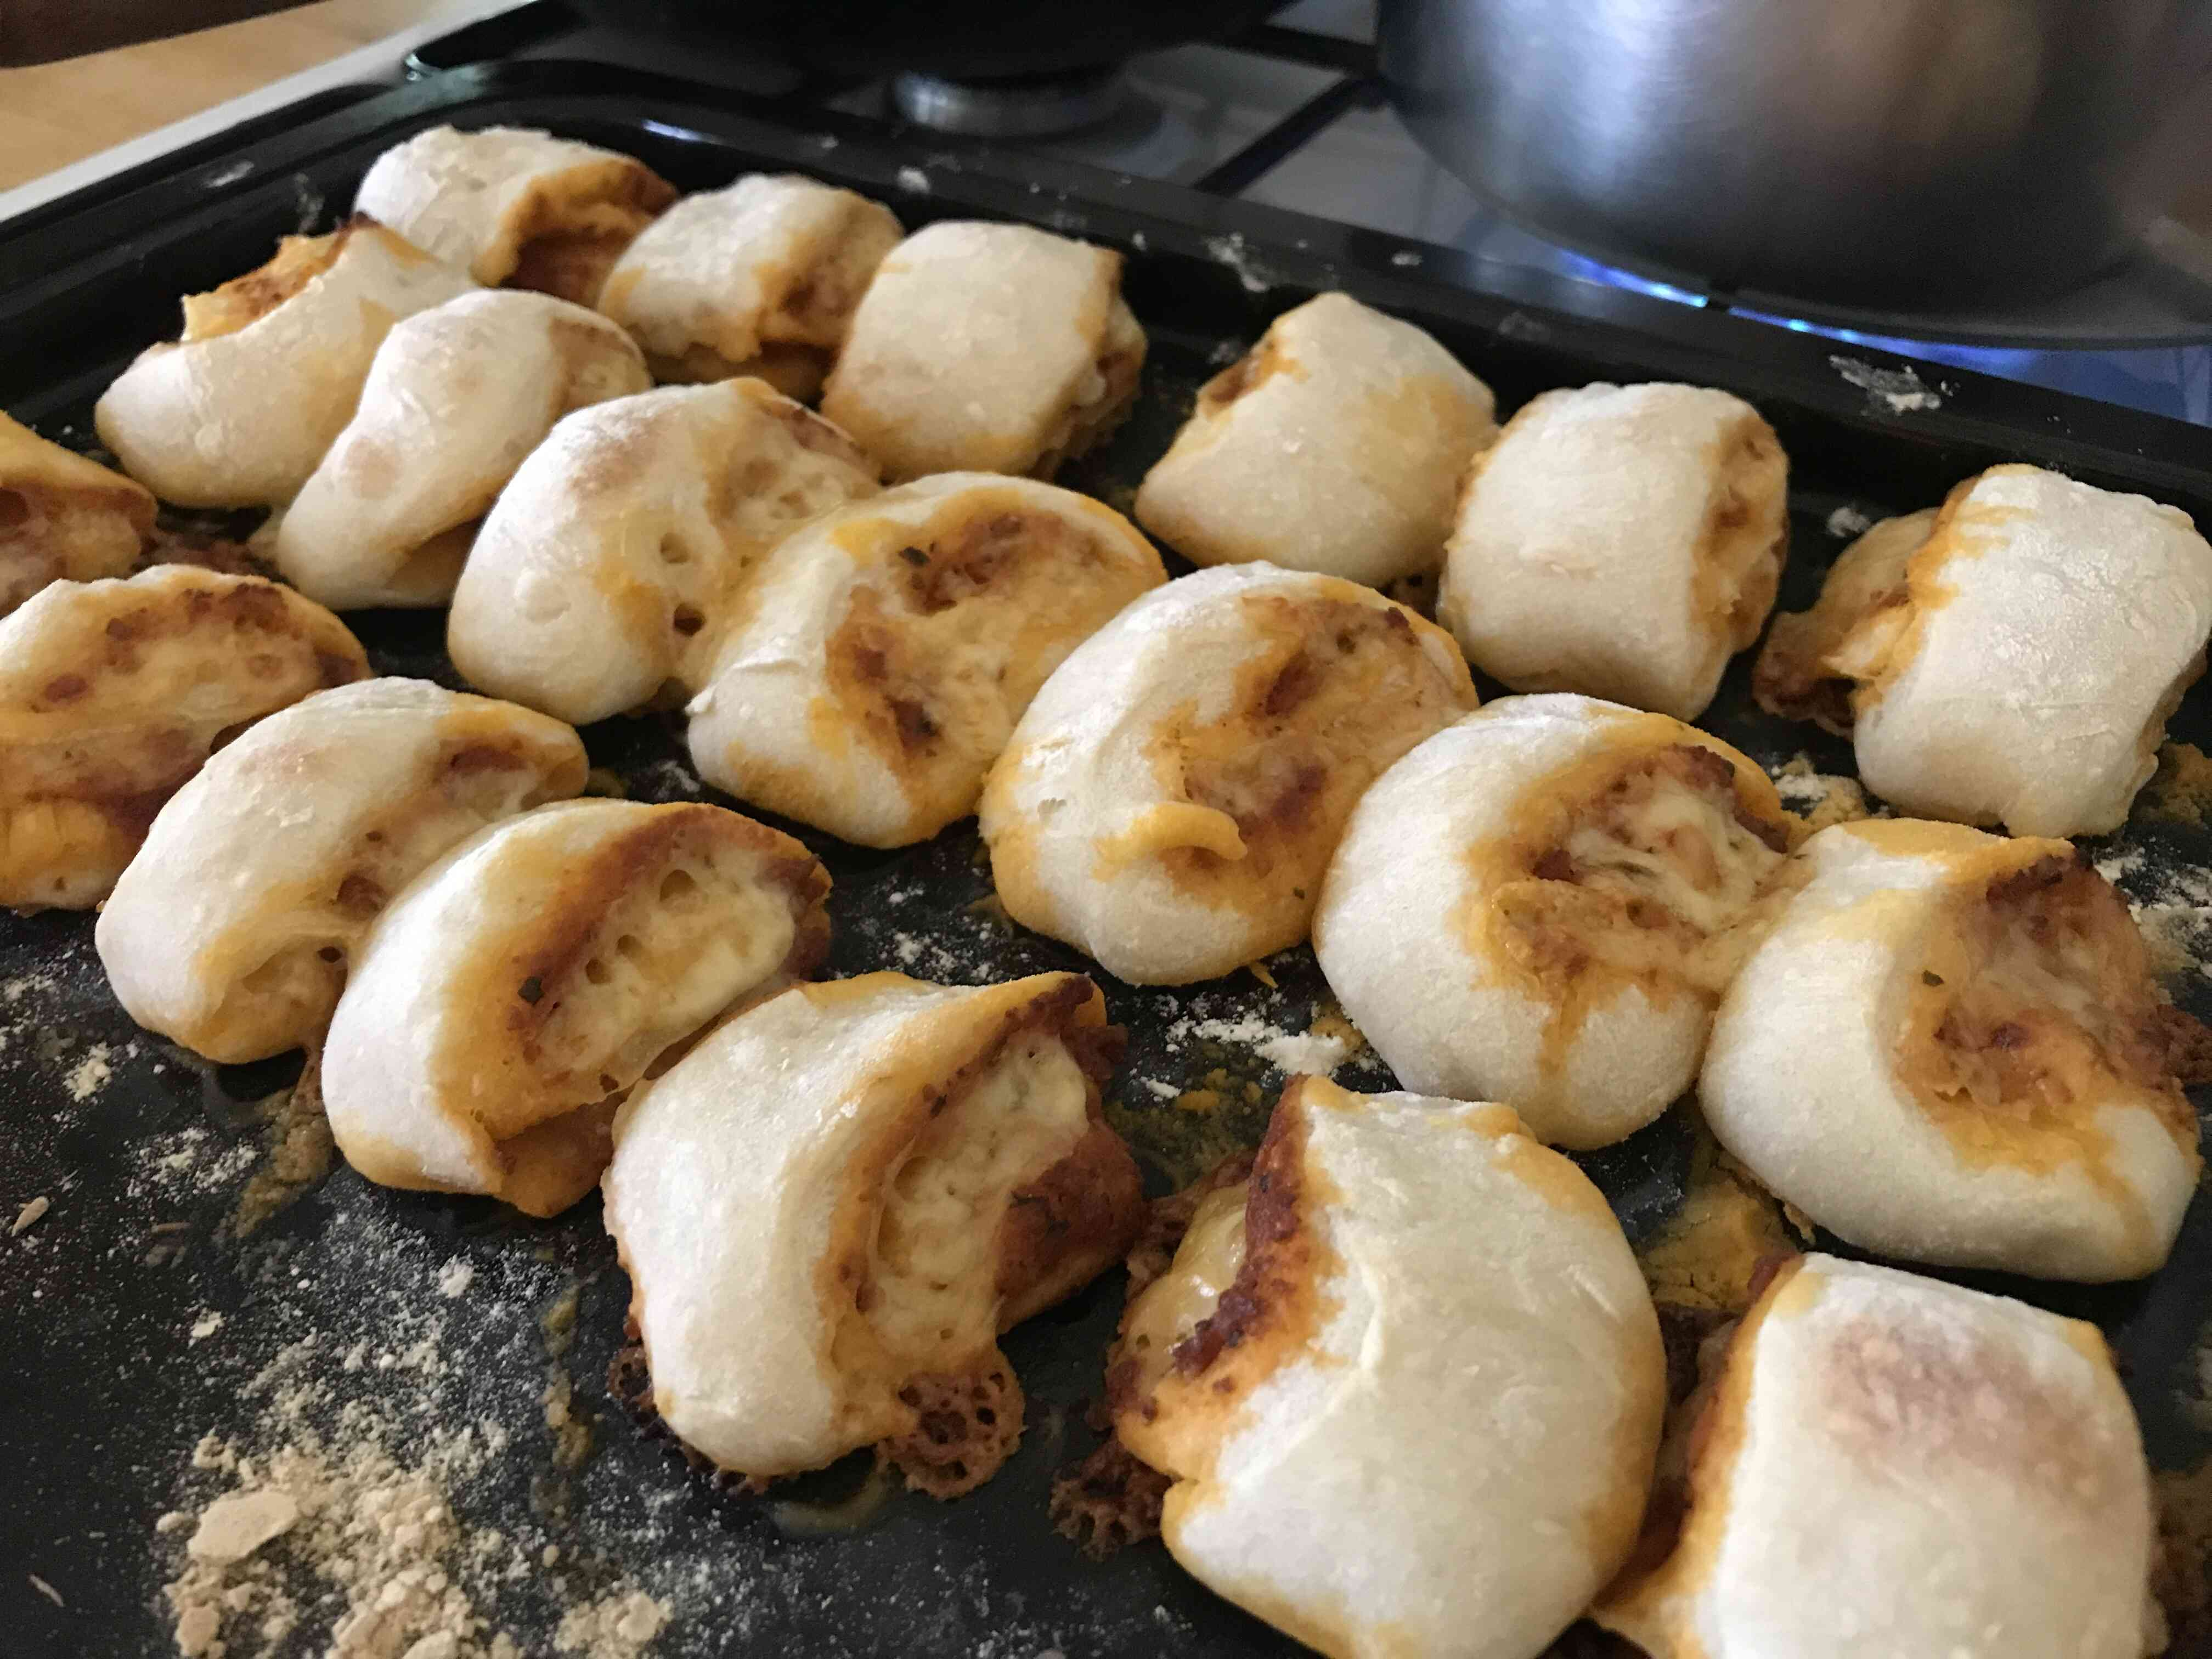
\includegraphics[height = 5cm]{media/pizzabroetchen.JPG}	\\
								&	\\
		\textbf{Beschreibung}	&	Stets ein sehr guter Snack zum Mitbringen zu einer Einladung, welcher einfach zuzubereiten ist und vielseitig angepasst werden kann.\\
								&	\\
		\begin{tabular}[t]{rr}
			\textbf{Zutaten}	\\
			Für 1 kg 			\\
			Für 20-30 Pizzabrötchen	\\
		\end{tabular}			&	\begin{tabular}[t]{llll}
										500 g & Weizenmehl 550er \\
										300 ml & Wasser \\
										1 TL & Salz \\
										1 g & Trockenhefe \\
										60 g & Tomatenpesto (getrocknete Tomaten, Hartkäse, \\ & Olivenöl, Basilikum, Knoblauch) \\
										100 g & Käse, nach Geschmack   							
									\end{tabular}	\\
		\textbf{Variationen}	&	\begin{itemize}[nosep]
										\item mit Basilikum-Pesto und Cashew-Kernen
									\end{itemize}	\\
		\textbf{Passendes}		&	\begin{itemize}[nosep]
										\item ...
									\end{itemize}	\\	
		% für zweiseitiges Rezept entkommentieren!
	\end{tabularx}
	\newpage
	\begin{tabularx}{\textwidth}{r|L}

									
		\begin{tabular}[t]{rr}
			\textbf{Zubereitung}	\\
			Vorbereitungszeit: 20 min	\\
			Backtemperatur: 250°C	\\
			Backzeit: 10-15 min
		\end{tabular}			&	\begin{enumerate}[nosep]
										\item Stelle den Basis-Hefeteig nach Rezept \ref{hefeteig_grundrezept} her.
										\item Teile den Teig in zwei gleiche Stücke und drücke beide auf einer bemehlten Arbeitsfläche zu einem Rechteck von ca. 10x40cm aus.
										\item Streiche das Pesto auf den Rechtecken aus und lege den Käse darauf, lasse jedoch an der langen Seite eine Rand von ca. 2cm frei!
										\item Wenn alles bereit zum Aufrollen des Teige ist, bestreiche den freien Teigsteifen mit Wasser, sodass er sehr gut klebt.
										\item Rolle von der anderen langen Seite aus den Teig auf und verschließe die Rolle mit dem gut haftenden befeuchteten Teigstreifen!
										\item Schneide nun jede Teigrolle in 10 Pizzabrötchen und lege diese mit einer gut bemehlten Seite auf ein Backblech.
										\item Backe alles bei 250°C für 10-15 min, bis der gewünschte Bräunungsgrad erreicht ist.
									\end{enumerate}	\\
	\end{tabularx}
	\newpage

%----------------------------------<Gebäck>--------------------------------------

\chapter{Gebäck}
\newpage

	%----------------------------------<Grundteige>--------------------------------------

	\section{Grundteige}
	\newpage

		% Rezept für Mürbeteig

		\subsection{Mürbeteig}

		% hier sollte noch ein Bild hinein

		\begin{tabularx}{\textwidth}{r|L}
			\textbf{Beschreibung}	&	Der wahrscheinlich einfachste süße Teig, welcher in einer Vielzahl von Süßgebäck in der ein oder anderen Form vorkommt.\\
									&	\\
			\begin{tabular}[t]{rr}
				\textbf{Zutaten}	\\
				Für 700 g Teig		\\
			\end{tabular}		
									&	\begin{tabular}[t]{ll}
									 		300 g	&	Mehl	\\
											200 g	&	Butter	\\
											1		&	Ei		\\
											100 g	&	Zucker	\\	
										\end{tabular}	\\
		%							&	\\
		%	\textbf{Variationen}	&	\begin{itemize}[nosep]
		%									\item
		%								\end{itemize}	\\
		%							&	\\	
		%	\textbf{Passendes}		&	\begin{itemize}[nosep]
		%									\item
		%								\end{itemize}	\\
									&	\\
			\textbf{Zubereitung}	&	\begin{enumerate}[nosep]
											\item Gib Butter und Zucker in die Teigschüssel und verrühre die Masse gleichmäßig.
											\item Füge das Mehl und das Ei hinzu.
											\item Knete den Mürbeteig kurz mit den Händen, bis er homogen ist.
											\item Stelle den fertigen Teig vor dem Weiterverarbeiten in den Kühlschrank.
										\end{enumerate}	\\
									&	\\
		\end{tabularx}
		\newpage

		%-------------------------------------------------------------------------

		% Rezept für Hefeteig

		\subsection{Hefeteig} \label{hefeteig_grundrezept}
		
		\begin{tabularx}{\textwidth}[t]{r|L}
									&	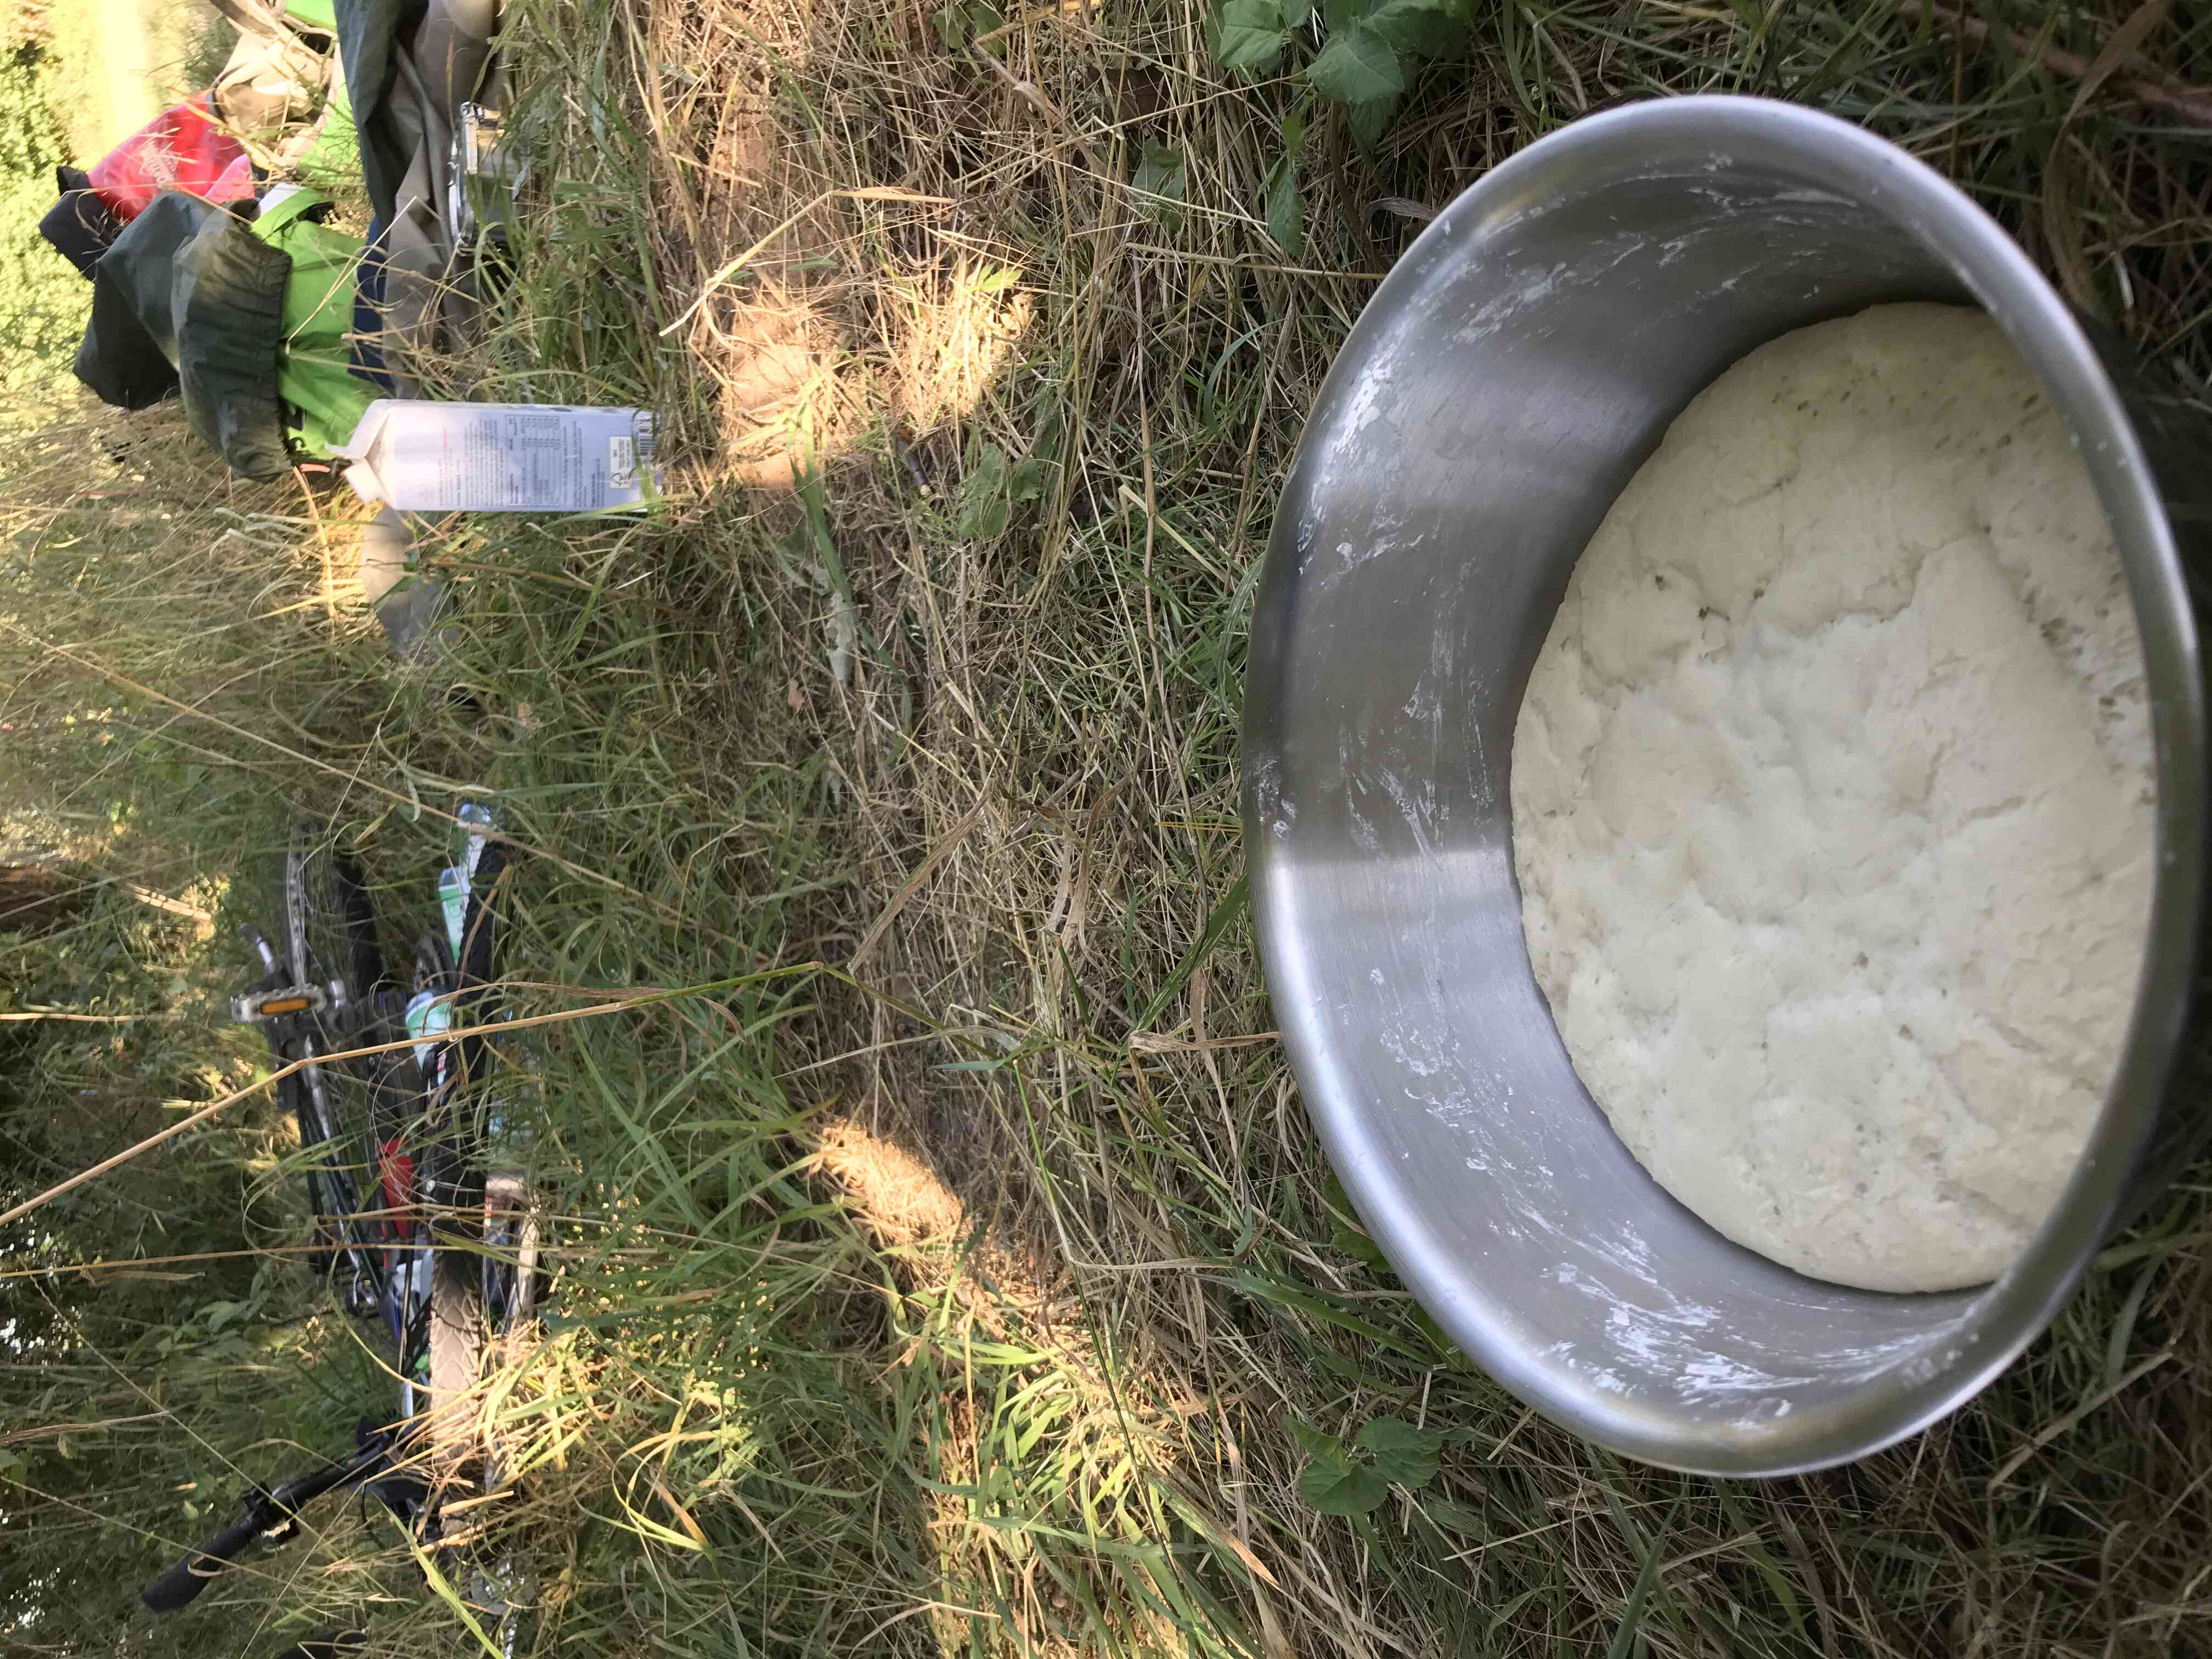
\includegraphics[height = 5cm, angle = 270]{media/hefeteig_reise.JPG}	\\
									&	\\
			\textbf{Beschreibung}	&	Dieses Basisrezept kann eigentlich immer verwendet werden, wenn man einen ganz „normalen“ Hefeteig haben möchte! \\
									&	Folgendes kann damit gemacht werden: Pizza, Stockbrot, Brötchen, Pitas, Baguette … \\
									&	\\
			\begin{tabular}[t]{rr}
				\textbf{Zutaten}	\\
				Für ~800 g Teig		\\
			\end{tabular}			&	\begin{tabular}[t]{llll}
											500 g	&	Weizenmehl 550er	&	\\
											300 g	&	Wasser				&	Wasser zu Mehl: $0,6 = 60\%$	\\
											10 g	&	Salz				&	Salz zu Mehl: $0,02 = 2\%$	\\
											1-5 g	&	Frischhefe		&	oder 0,5-1 g Trockenhefe\\			
										\end{tabular}	\\
									&	\\
			\textbf{Variationen}	&	\begin{itemize}[nosep]
											\item 4/5 Vollkornmehl und 1/5 550er
										\end{itemize}	\\
									&	\\	
			\textbf{Passendes}		&	\begin{itemize}[nosep]
											\item
										\end{itemize}	\\
									&	\\
			\textbf{Zubereitung}	&	\begin{enumerate}[nosep]
											\item	Falls frische Hefe verwendet wird, löse diese in dem Wasser auf.
											\item 	Gib das Mehl, das Salz und falls verwendet die Trockenhefe in eine Schüssel und vermische es kurz.
											\item 	Füge das Wasser hinzu und verrühre die Masse grob, bis das Wasser gebunden ist.
											\item 	Knete nun den Teig auf einer Arbeitsfläche mit der Hand, bis er homogen und elastisch ist.
											\item 	Lasse den Teig für mindestens 4 und höchstens 24 Stunden gehen.
										\end{enumerate}	\\
									&	\\
		\end{tabularx}

		% Weitere Bilder zu Hefeteig

		\begin{figure}[h]
			\centering
			\begin{minipage}{0.49\textwidth}
				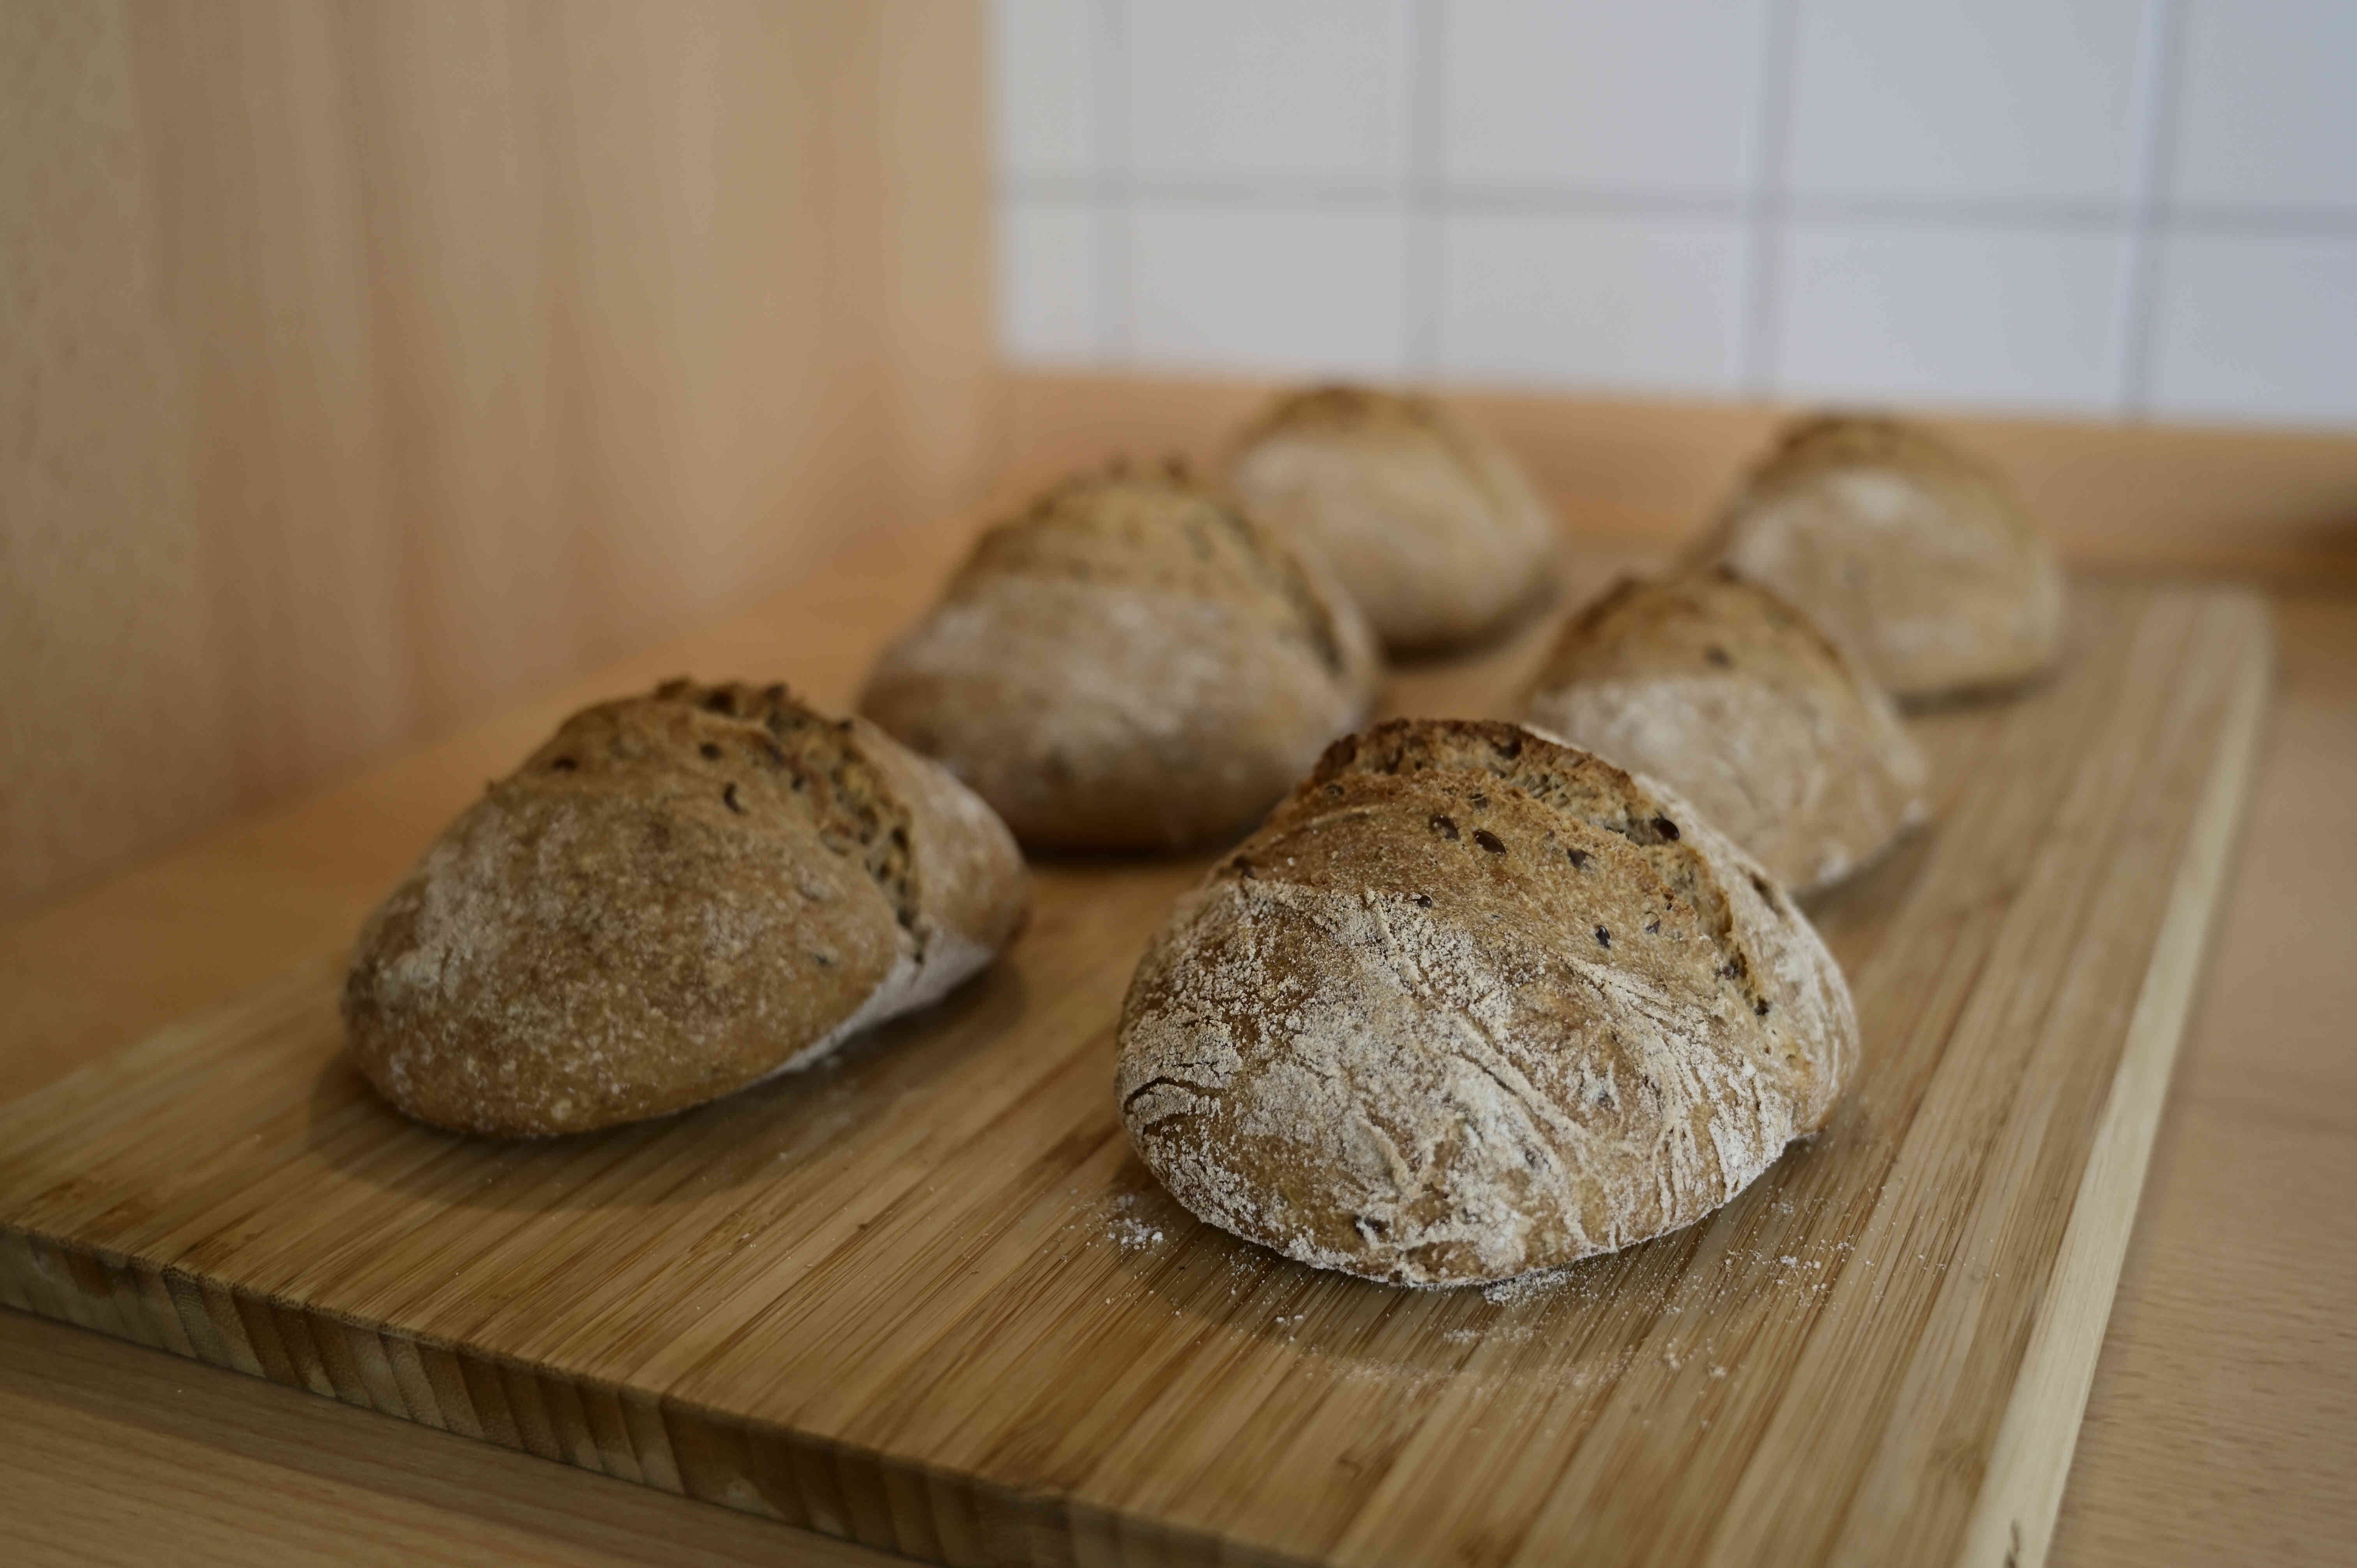
\includegraphics[width = \textwidth]{media/vollkorn_broetchen.jpg}
				\caption{Vollkorn-Brötchen}
			\end{minipage}
			\begin{minipage}{0.5\textwidth}
				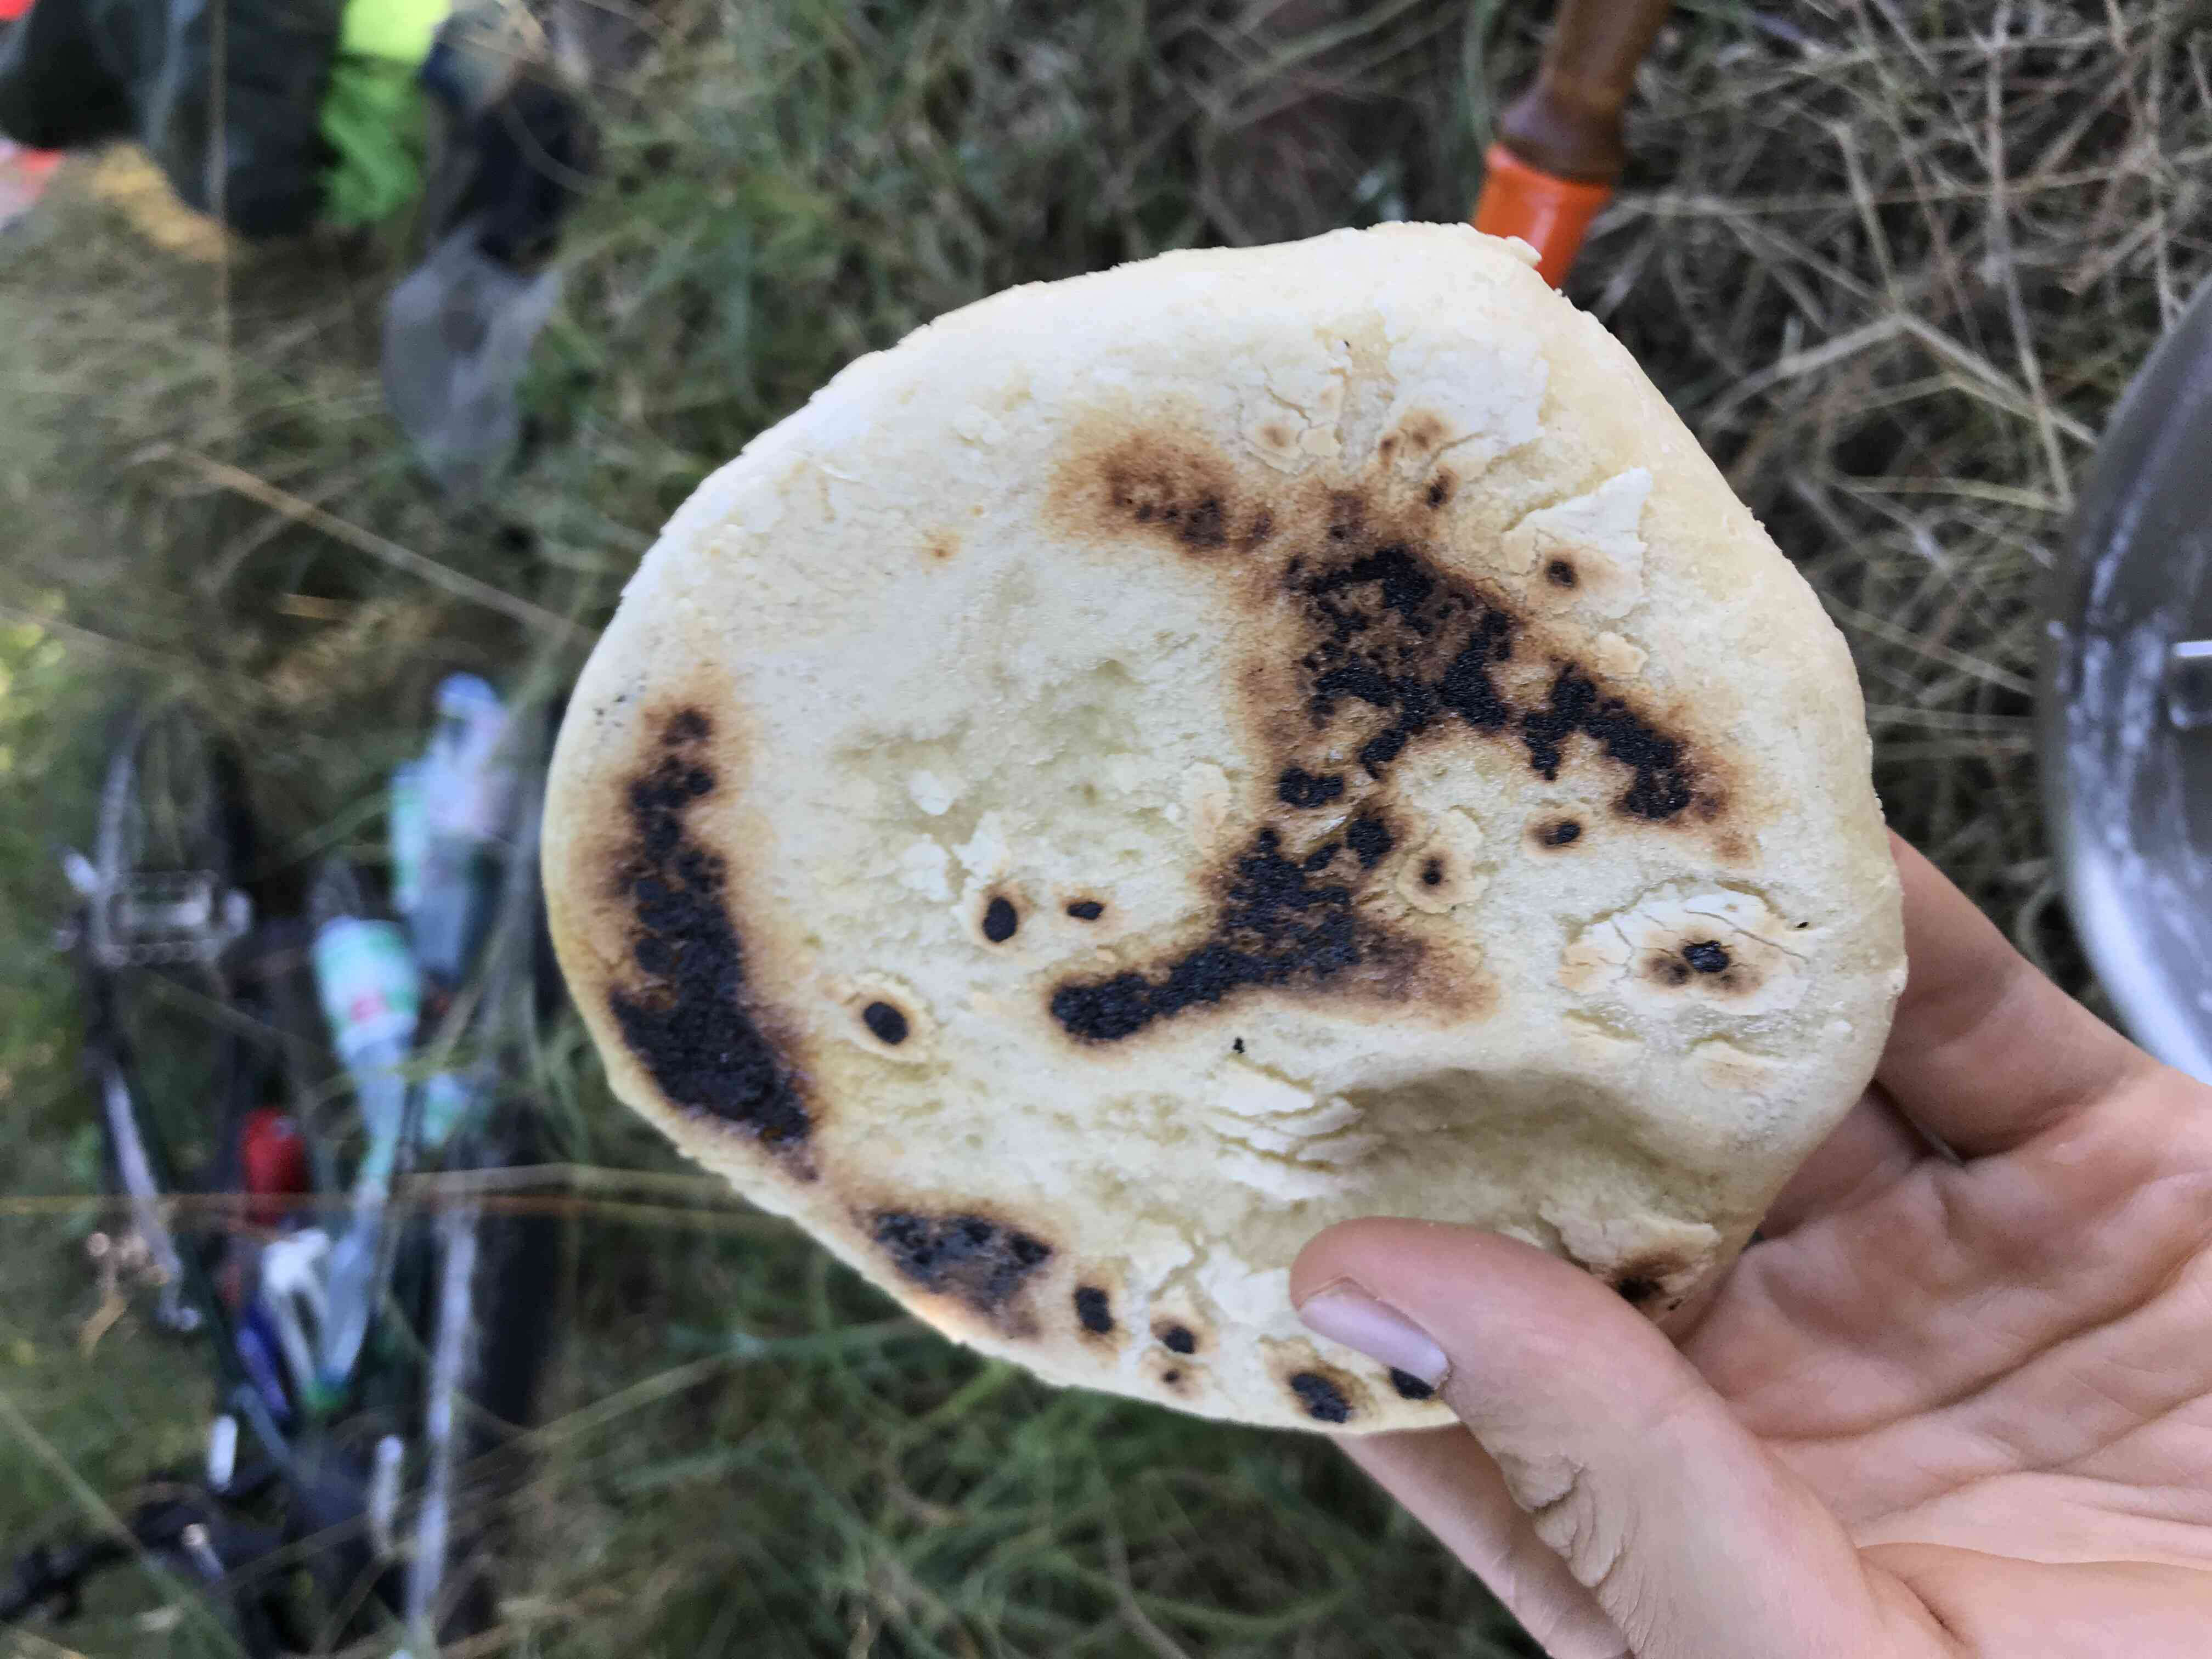
\includegraphics[width = \textwidth]{media/Fladenbrot.JPG}
				\caption{Fladenbrot aus Pfanne}
			\end{minipage}
		\end{figure}


		
		\newpage

	\section{Brot}
	\newpage

	% Brötchen

	\subsection{Brötchen} \label{Broetchen}

	\begin{tabularx}{\textwidth}{r|L}
								& 	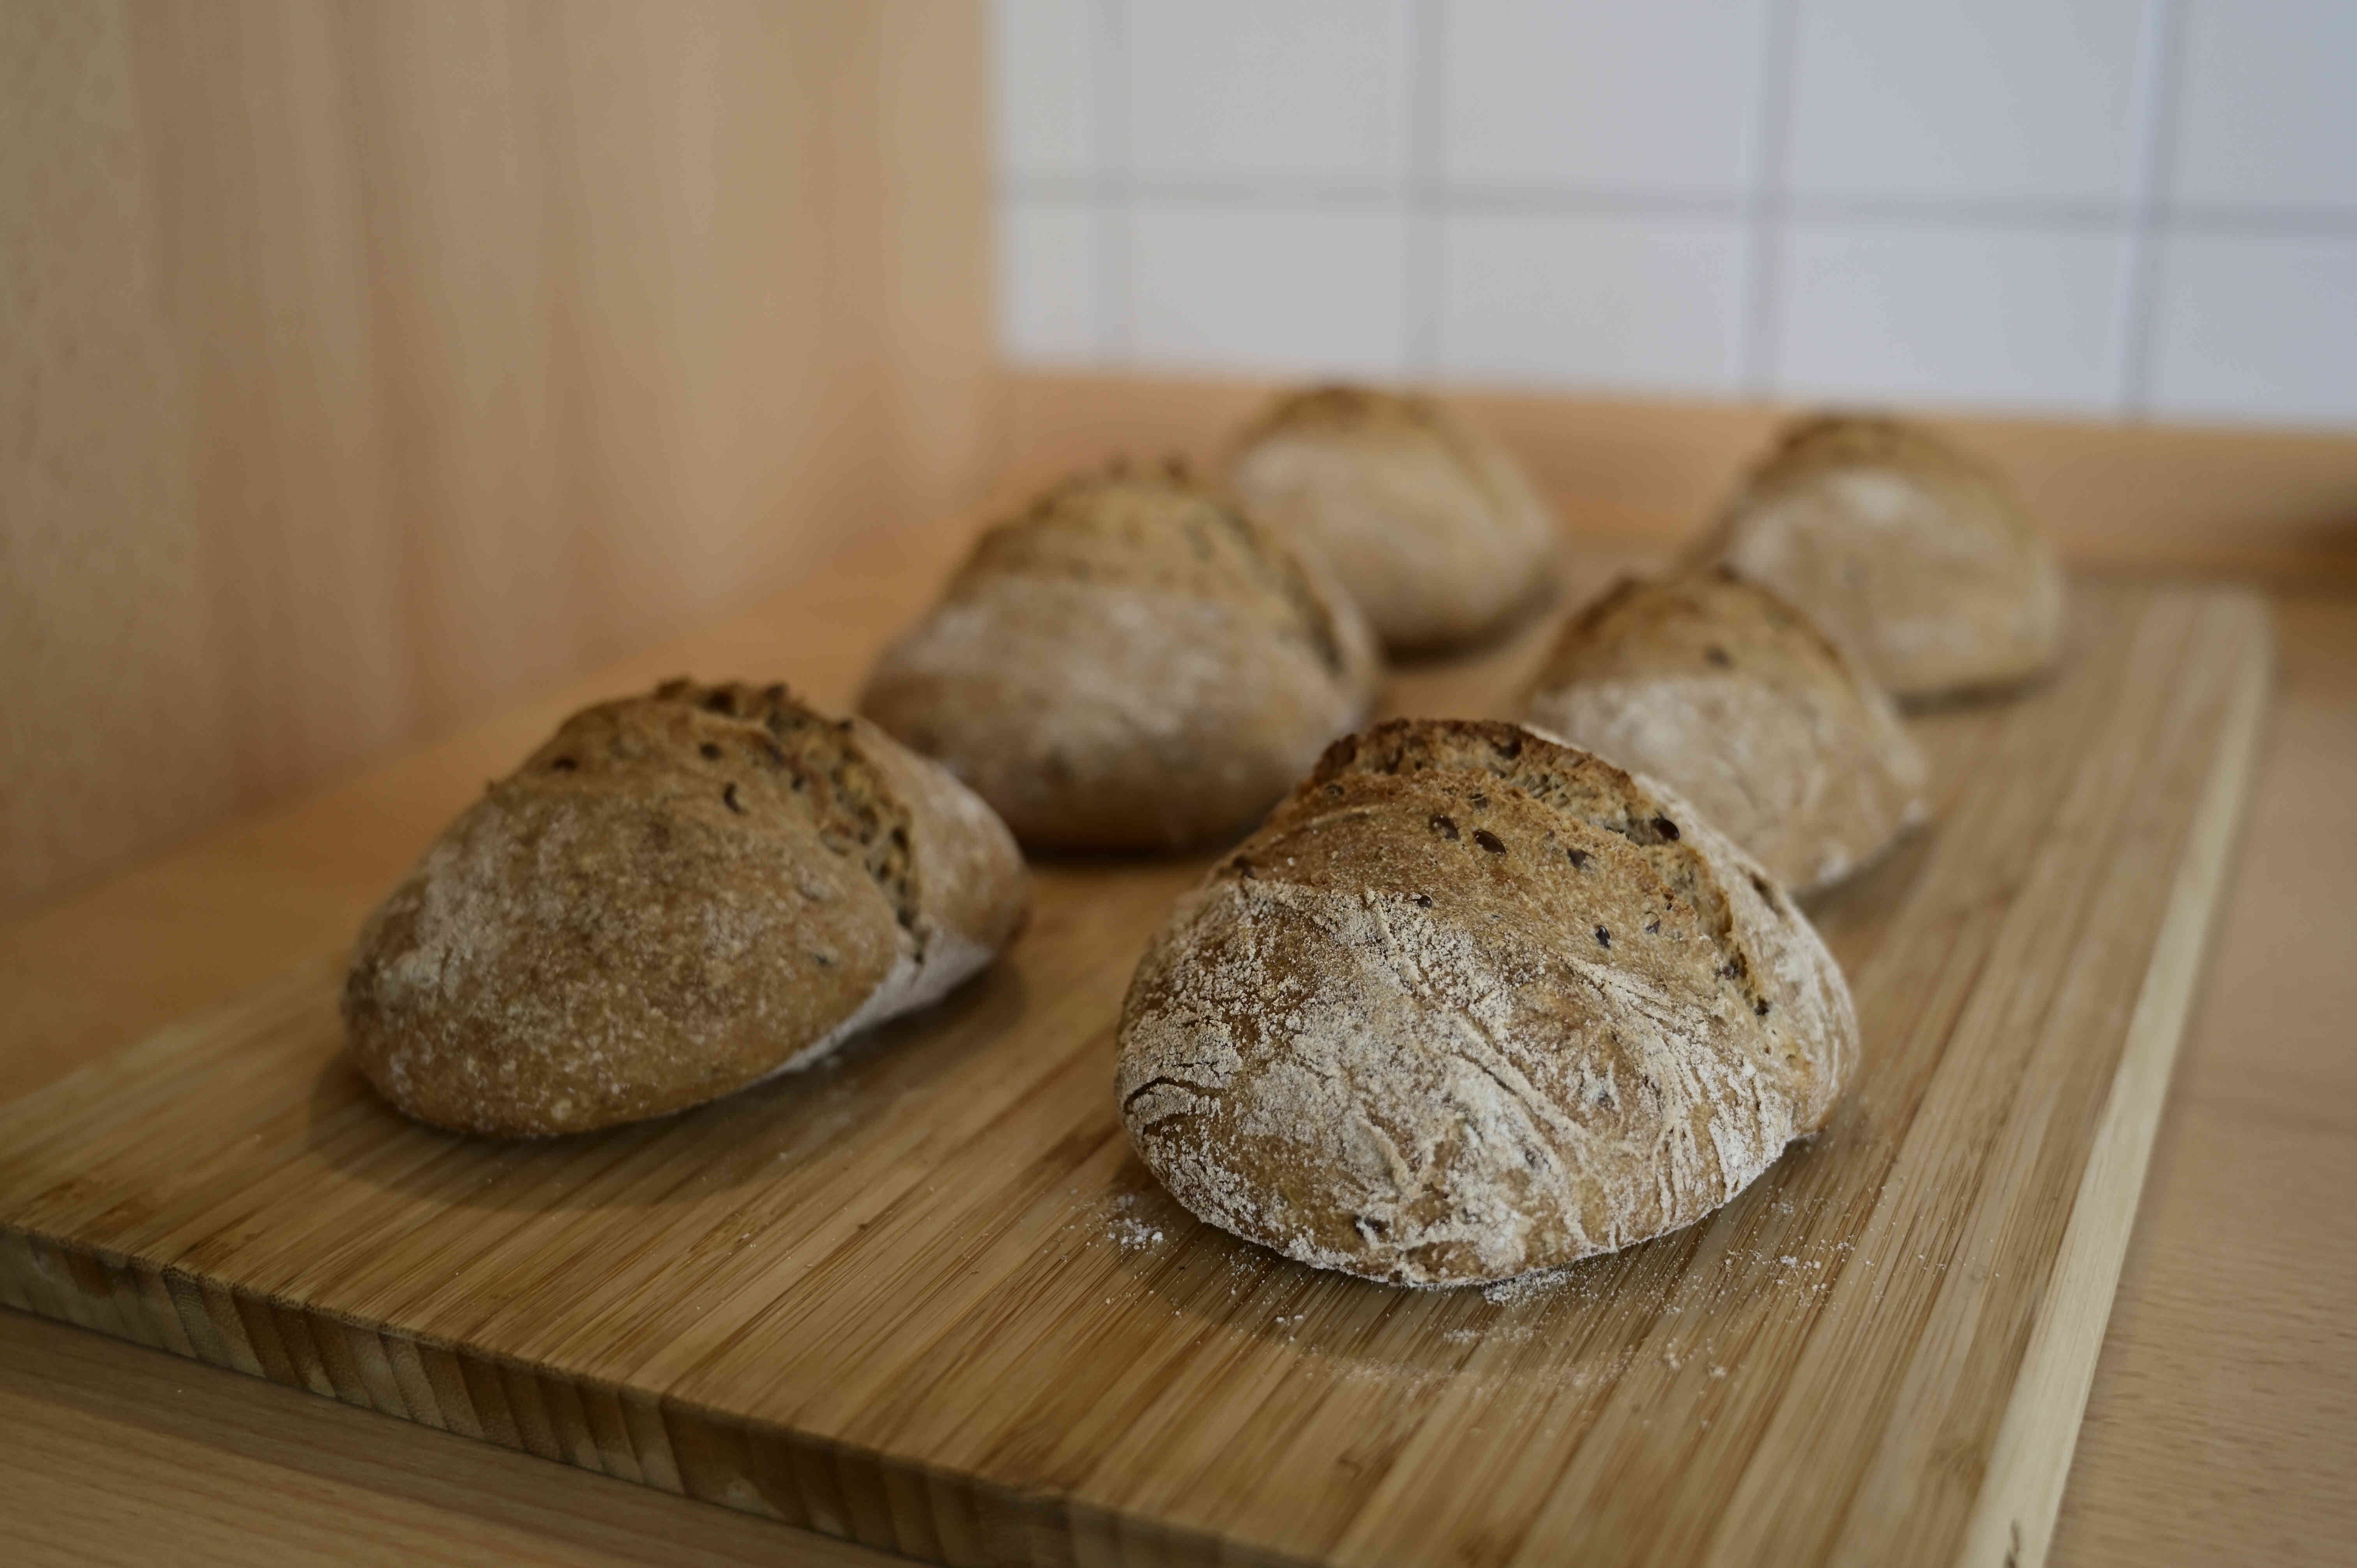
\includegraphics[height = 5cm]{media/vollkorn_broetchen.jpg}	\\
								&	\\
		\textbf{Beschreibung}	&	Kleine Brotportionen, welche ein besseres Kruste zu Volumen Verhältnis haben, als 										Brotscheiben!\\
								&	\\
		\begin{tabular}[t]{rr}
			\textbf{Zutaten}	\\
			Für ~1700 g 			\\
			Für 16 Brötchen	\\
		\end{tabular}			&	\begin{tabular}[t]{llll}
										1 kg & Mehl, diverses \\	
										600 g & Wasser \\
										100 g & Kerne, Saaten, Rosinen \\
										20 g & Salz \\
										0,5 g & Trockenhefe \\						
									\end{tabular}	\\
								&	\\
		\textbf{Variationen}	&	\begin{itemize}[nosep]
										\item ...
									\end{itemize}	\\
								&	\\	
		\textbf{Passendes}		&	\begin{itemize}[nosep]
										\item ...
									\end{itemize}	\\
								&	\\	
		\begin{tabular}[t]{rr}
			\textbf{Zubereitung}	\\
			Arbeitszeit: 20-30 min	\\
			Gehzeit: 6-12 h			\\
			Backzeit: 30-40 min		\\
			Backtemperatur: 220-250°C \\
		\end{tabular}			&	\begin{enumerate}[nosep]
										\item Bereite einen Hefeteig aus den Zutaten gemäß des Rezeptes \ref{hefeteig_grundrezept} zu.
										\item Nach der Gehzeit teile den Teig auf einer bemehlten Oberfläche in 16 Teile mit je ~100 g.
										\item Bringe die Brötchen in Form mit einer Technik der Wahl und lege sie mit genügend Mehl auf ein Backblech, wobei mit genügend Mehl kein Backpapier benötigt wird.
										\item Backe nun die Brötchen im Ofen mit den angegebene Temperaturen und Zeiten, wobei der angemessene Bräunungsgrad und der hohle Klang bei Klopfen auf die Unterseite die Kriterien für fertige Brötchen darstellen.
									\end{enumerate}	\\
		\end{tabularx}

		\begin{figure}
			\centering
			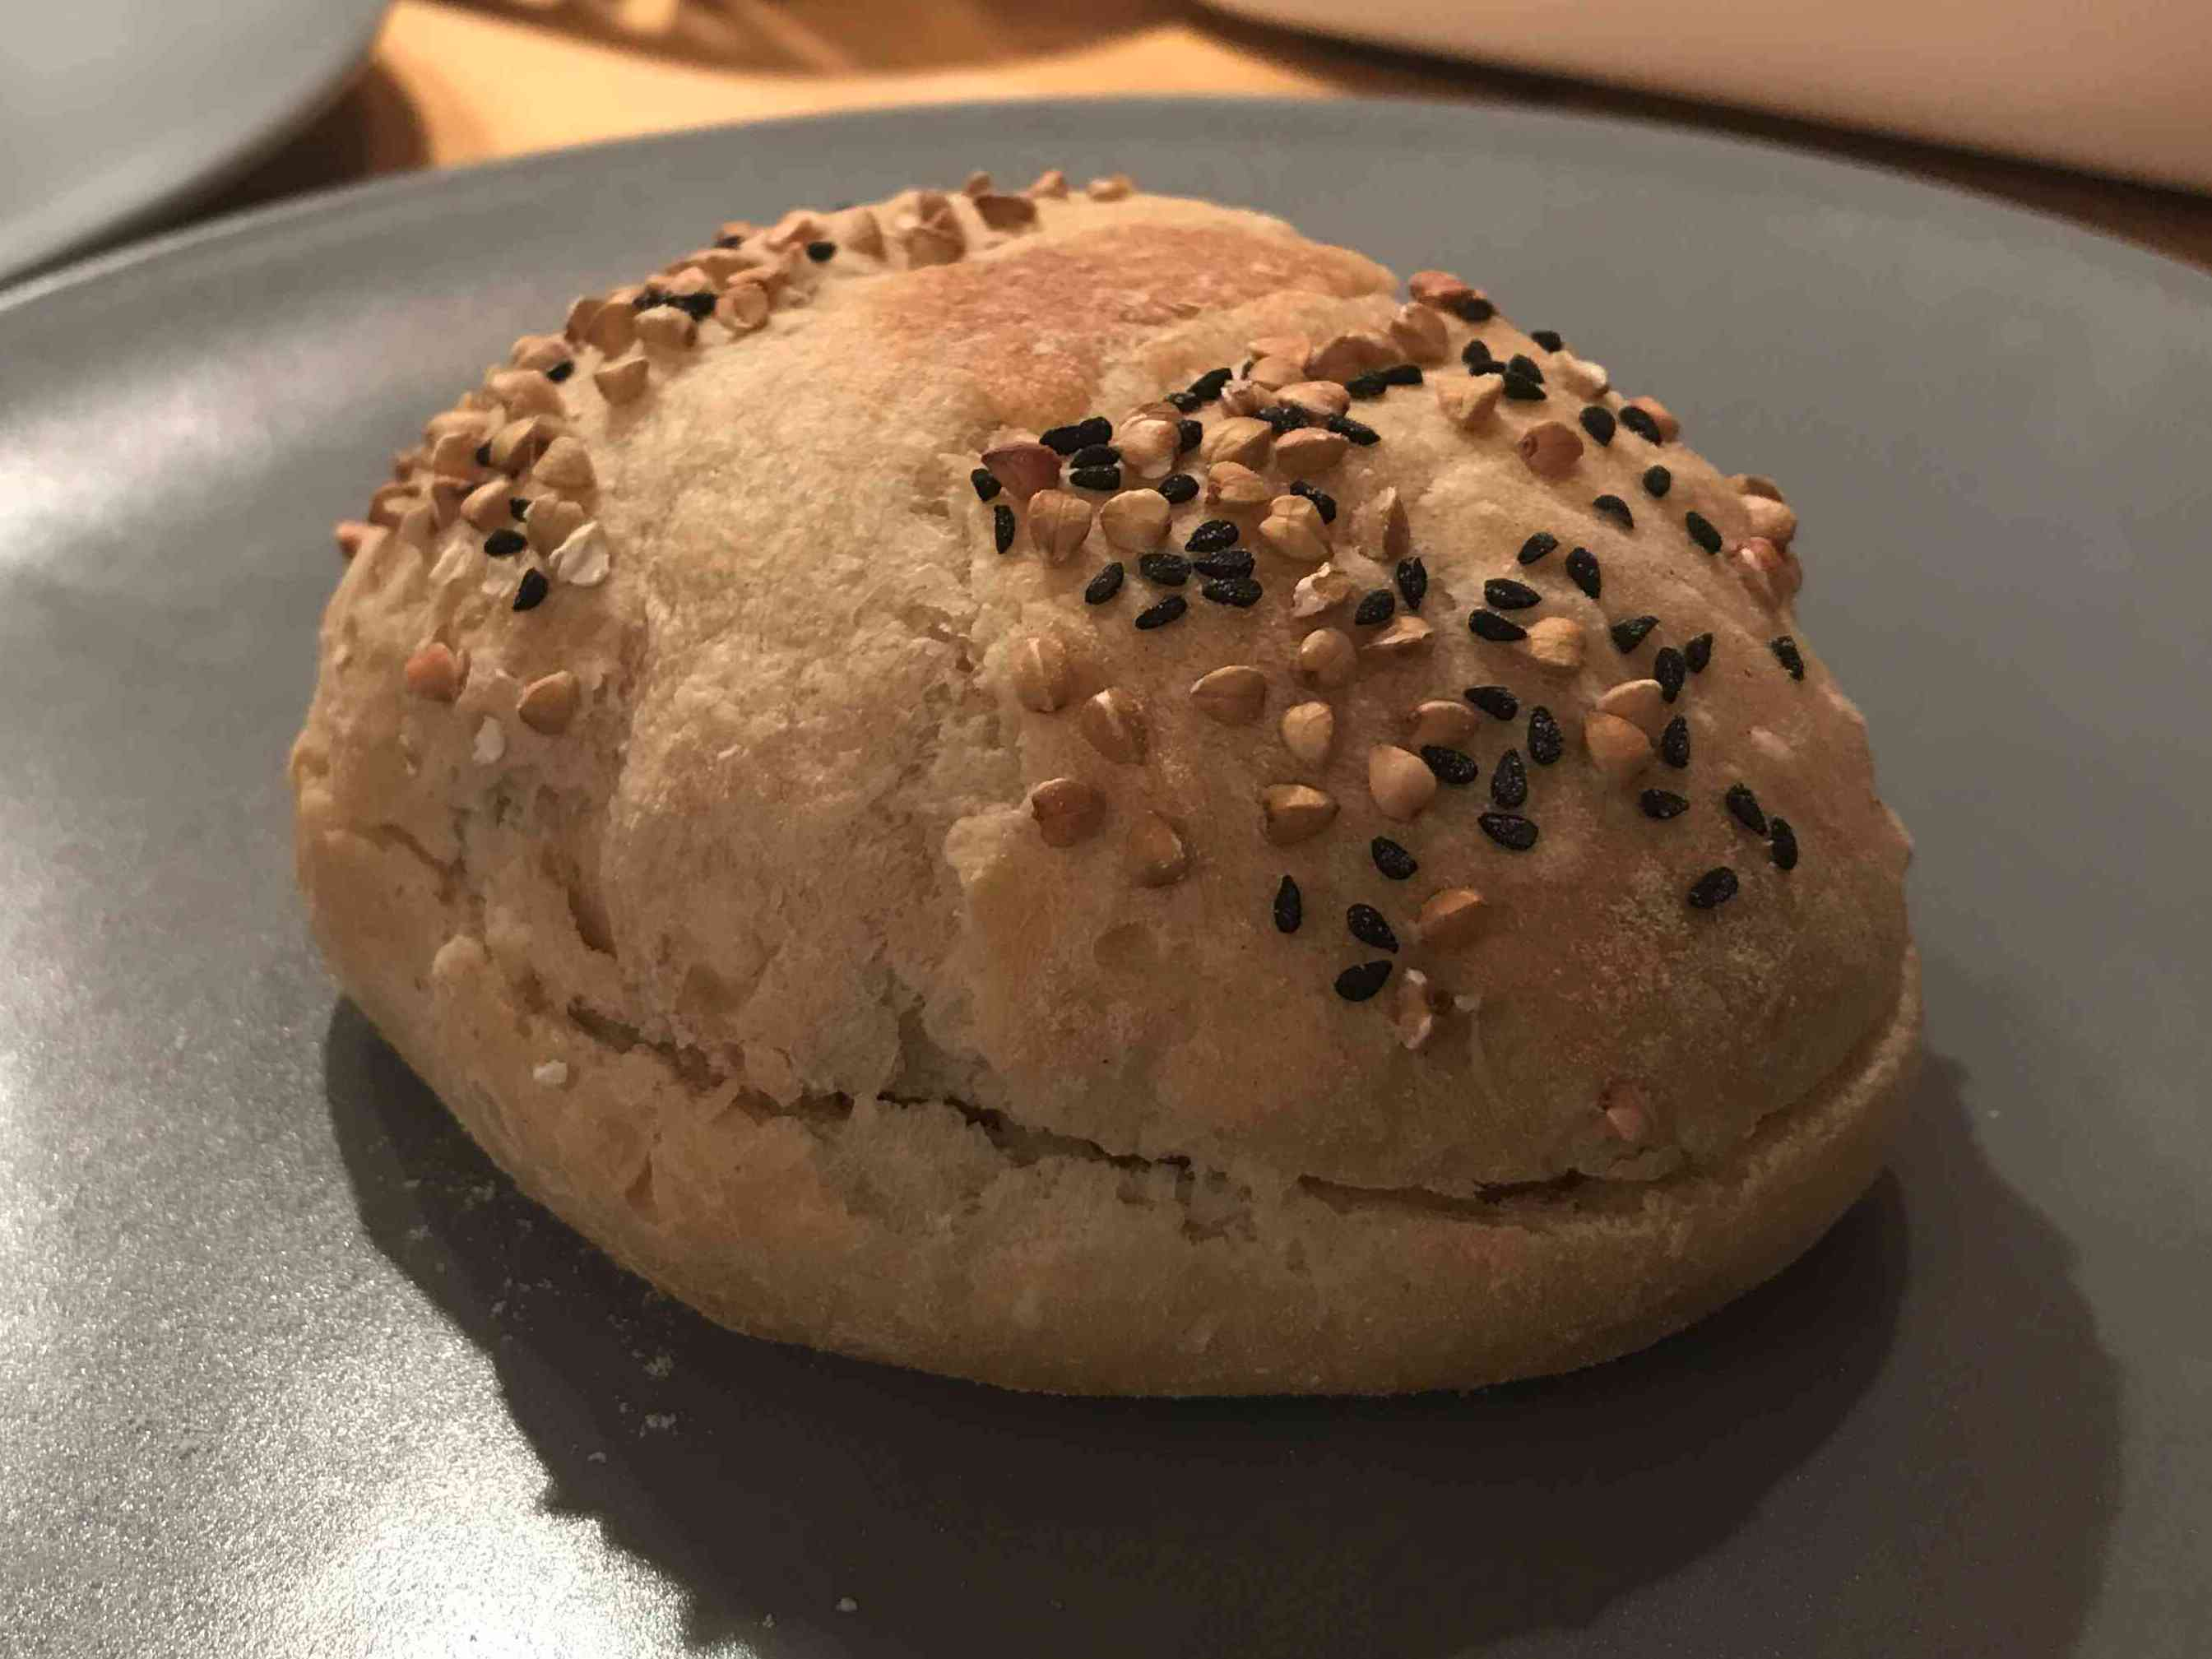
\includegraphics[width = 0.6\textwidth]{media/burger_broetchen.JPG}
		\end{figure}

		\newpage

		% Fladenbrot

		\subsection{Fladenbrot}	\label{fladenbrot}

		\begin{tabularx}{\textwidth}{r|L}
									& 	
\includegraphics[height = 5cm]{media/fladenbrot_flach.JPG}	\\
									&	\\
			\textbf{Beschreibung}	&	Die erste Zubereitung von Getreide, die der Mensch erfunden hat, war vermutlich Fladenbrot.\\
									& 	Wegen seiner Einfachheit sind Fladenbrote auf der ganzen Welt in den unterschiedlichsten Formen anzutreffen!\\
									&	\\
			\begin{tabular}[t]{rr}
				\textbf{Zutaten}	\\
				Für 480 g 			\\
				Für 4 Portionen	\\
			\end{tabular}			&	\begin{tabular}[t]{llll}
											320 g & Weizenmehl, 550er \\
											160 g & Wasser \\
											6 g & Salz \\						
										\end{tabular}	\\
									&	\\
			\textbf{Variationen}	&	\begin{itemize}[nosep]
											\item Naan-Brot
											\begin{tabular}{lll}
												60 ml & Joghurt \\
												1 EL & Olivenöl \\
												1 TL & Zucker \\
												bisschen Trockenhefe ?\\
												bis Konsistenz stimmt & Milch statt Wasser \\
											\end{tabular} 
										\end{itemize}	\\
									&	\\	
			\textbf{Passendes}		&	\begin{itemize}[nosep]
											\item Tex-Mex Wraps mit Bohnen, Crème Fraîche, Mais, Hackfleich und Salsa
											\item Salat, Gemüse, Soßen, Seitan 
										\end{itemize}	\\
									&	\\
		\end{tabularx}
									\newpage

		\begin{tabularx}{\textwidth}{r|L}										
			\begin{tabular}[t]{rr}
				\textbf{Zubereitung}	\\
				Arbeitszeit: 10 min	\\
				Gesamtzeit:	40 min		\\
			\end{tabular}			&	\begin{enumerate}[nosep]
											\item Gib Mehl, Salz, Wasser in ein Gefäß und vermenge alles grob.
											\item Knete nun den Teig am besten mit den Händen ordentlich, bis genug Spannung in das Gluten gebracht wurde.
											\item Lasse den Teig mindestens 30 min in einem abgeschlossenen Behälter ruhen, sodass er vom Austrocken bewahrt ist.
											\item Heize eine Pfanne ohne Öl auf mittlerer Hitze vor und drücke den Teig flach bis auf die Größe der zur Verfügung stehenden heißen Fläche.
											\item Backe das Fladenbrot von beiden Seiten 3-5 min, bis es einen guten Bräunungsgrad erreicht hat und durchgebacken ist.
										\end{enumerate}	\\
		\end{tabularx}

		\begin{figure}[h]
			\centering
			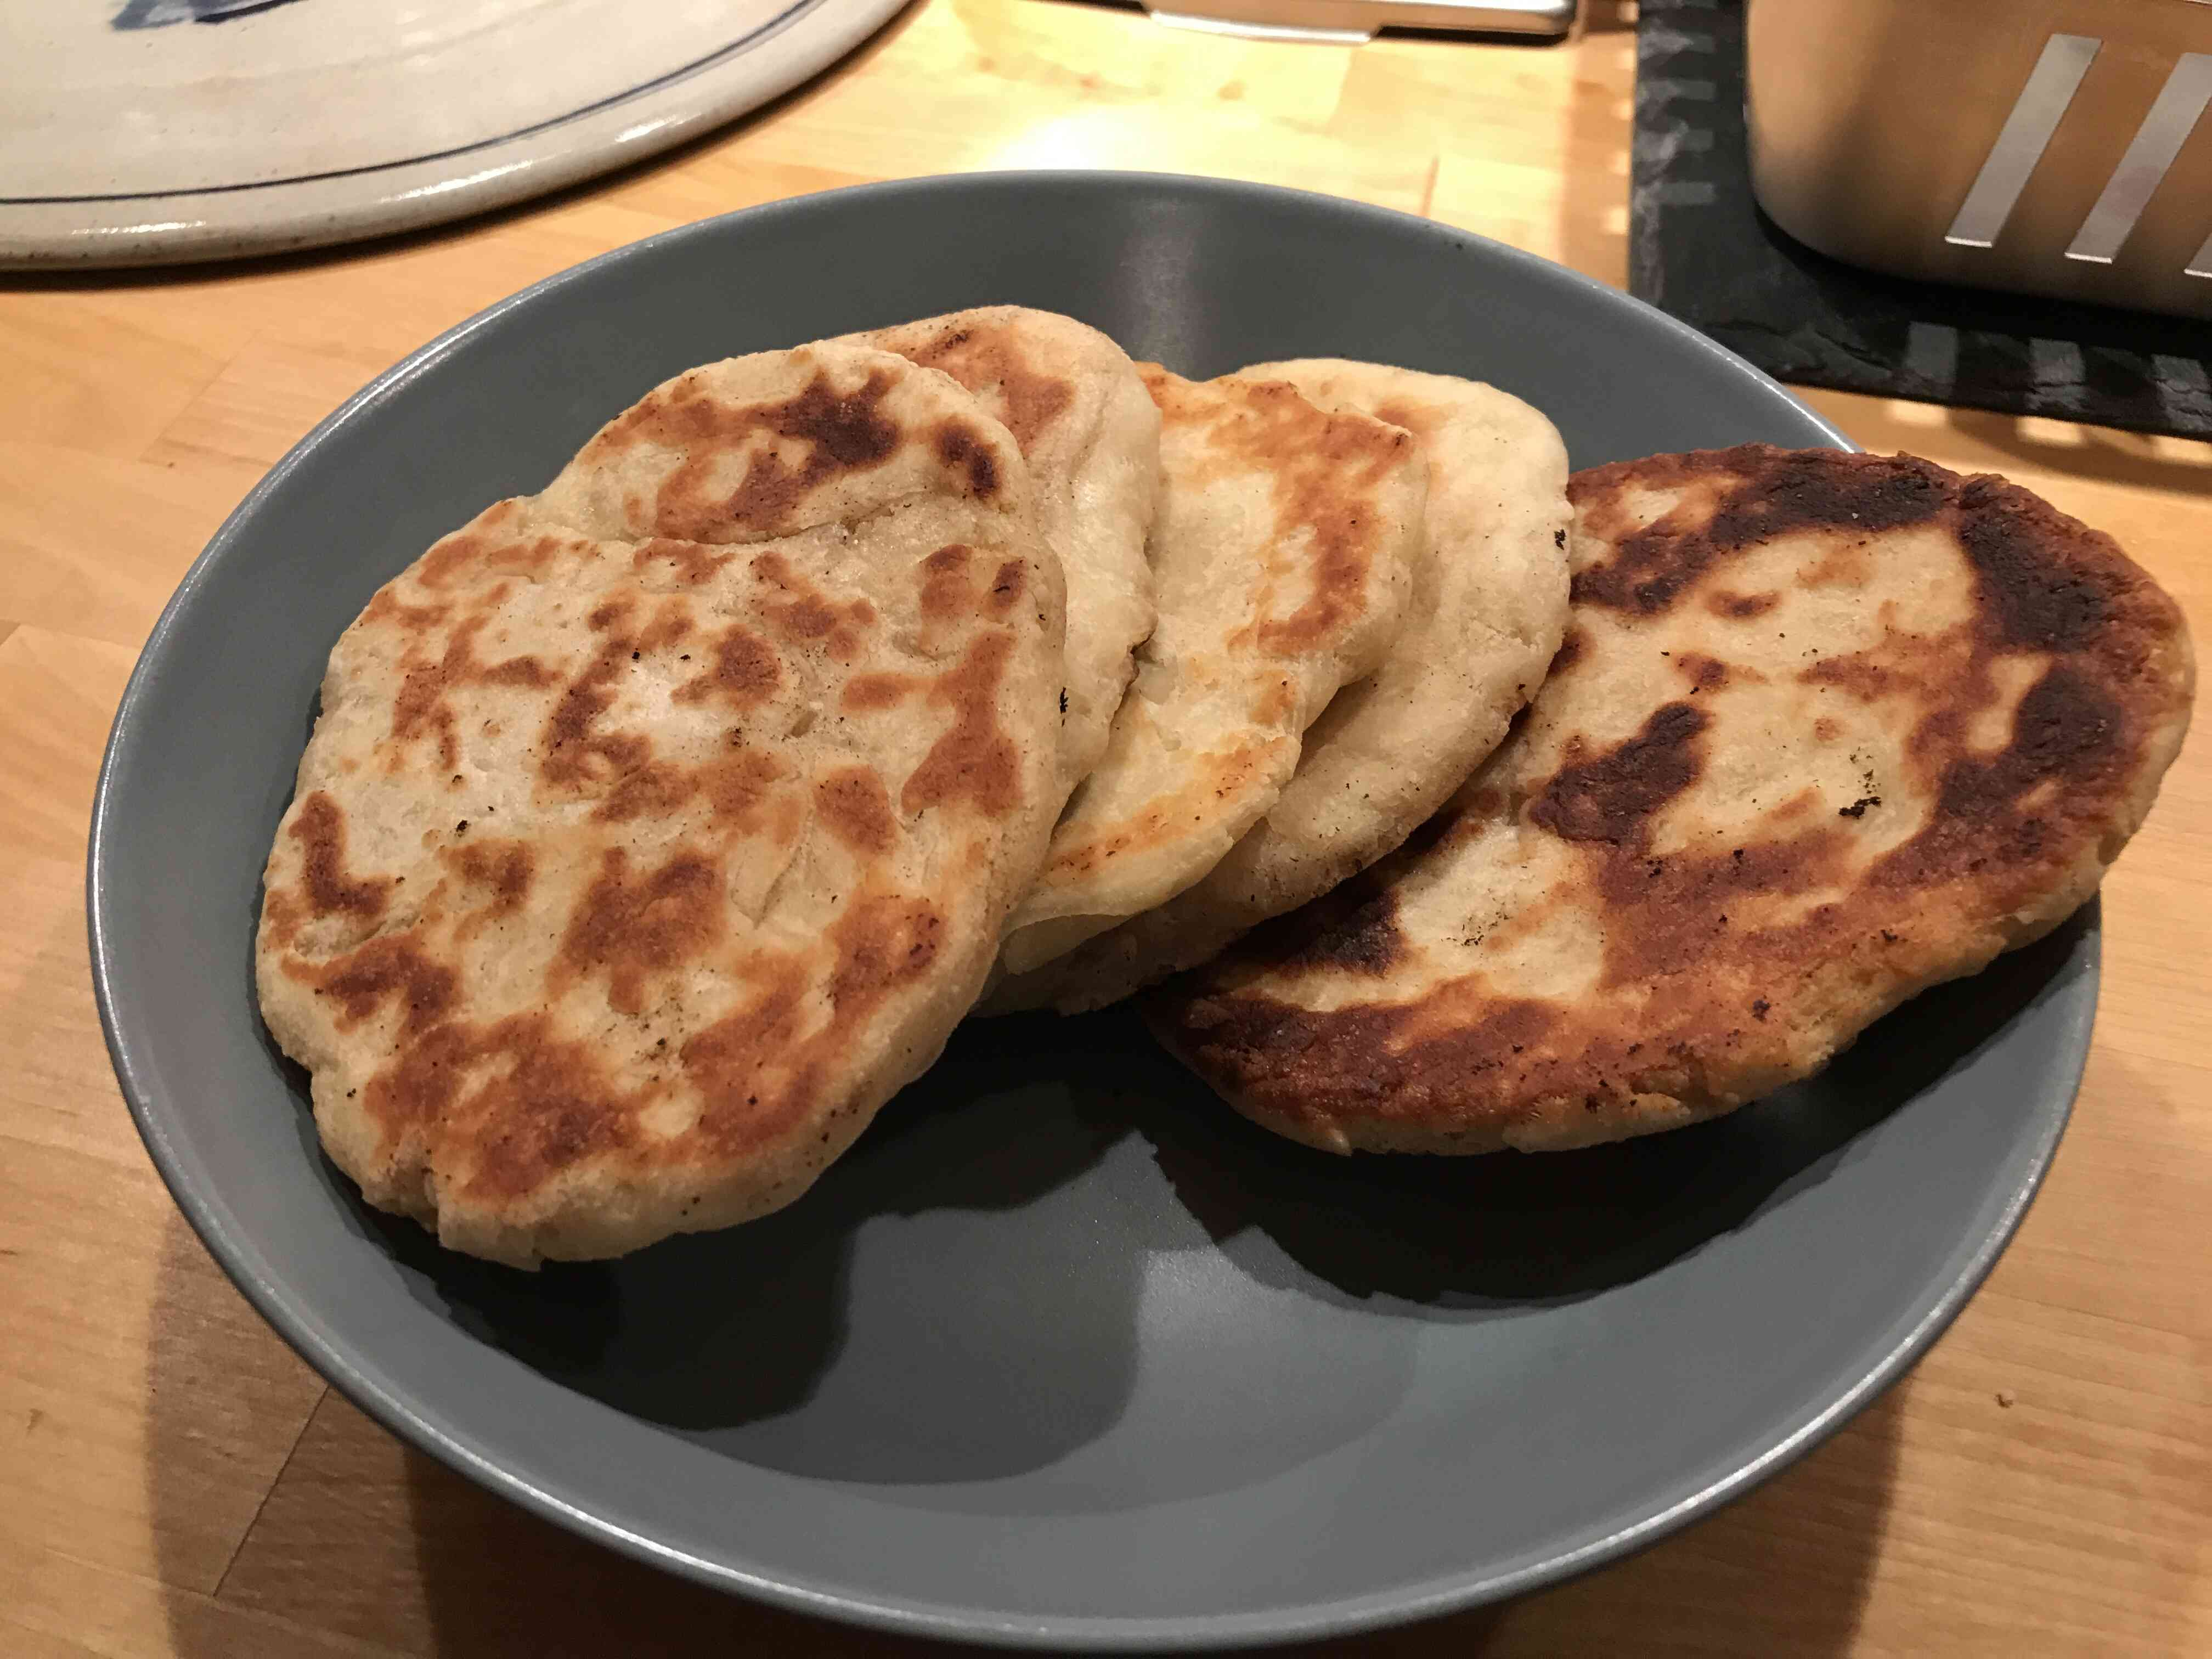
\includegraphics[width = 0.7\textwidth]{media/naan_brot.JPG}
			\caption{Naan-Brot als indische leicht süßliche Variante}
		\end{figure}

		\newpage

	%----------------------------------<Süßgebäck>--------------------------------------

	\section{Süßgebäck}
	\newpage

		% Rührkuchen

		\subsection{Rührkuchen}	\label{ruehrkuchen}

		\begin{tabularx}{\textwidth}{r|L}
									& 	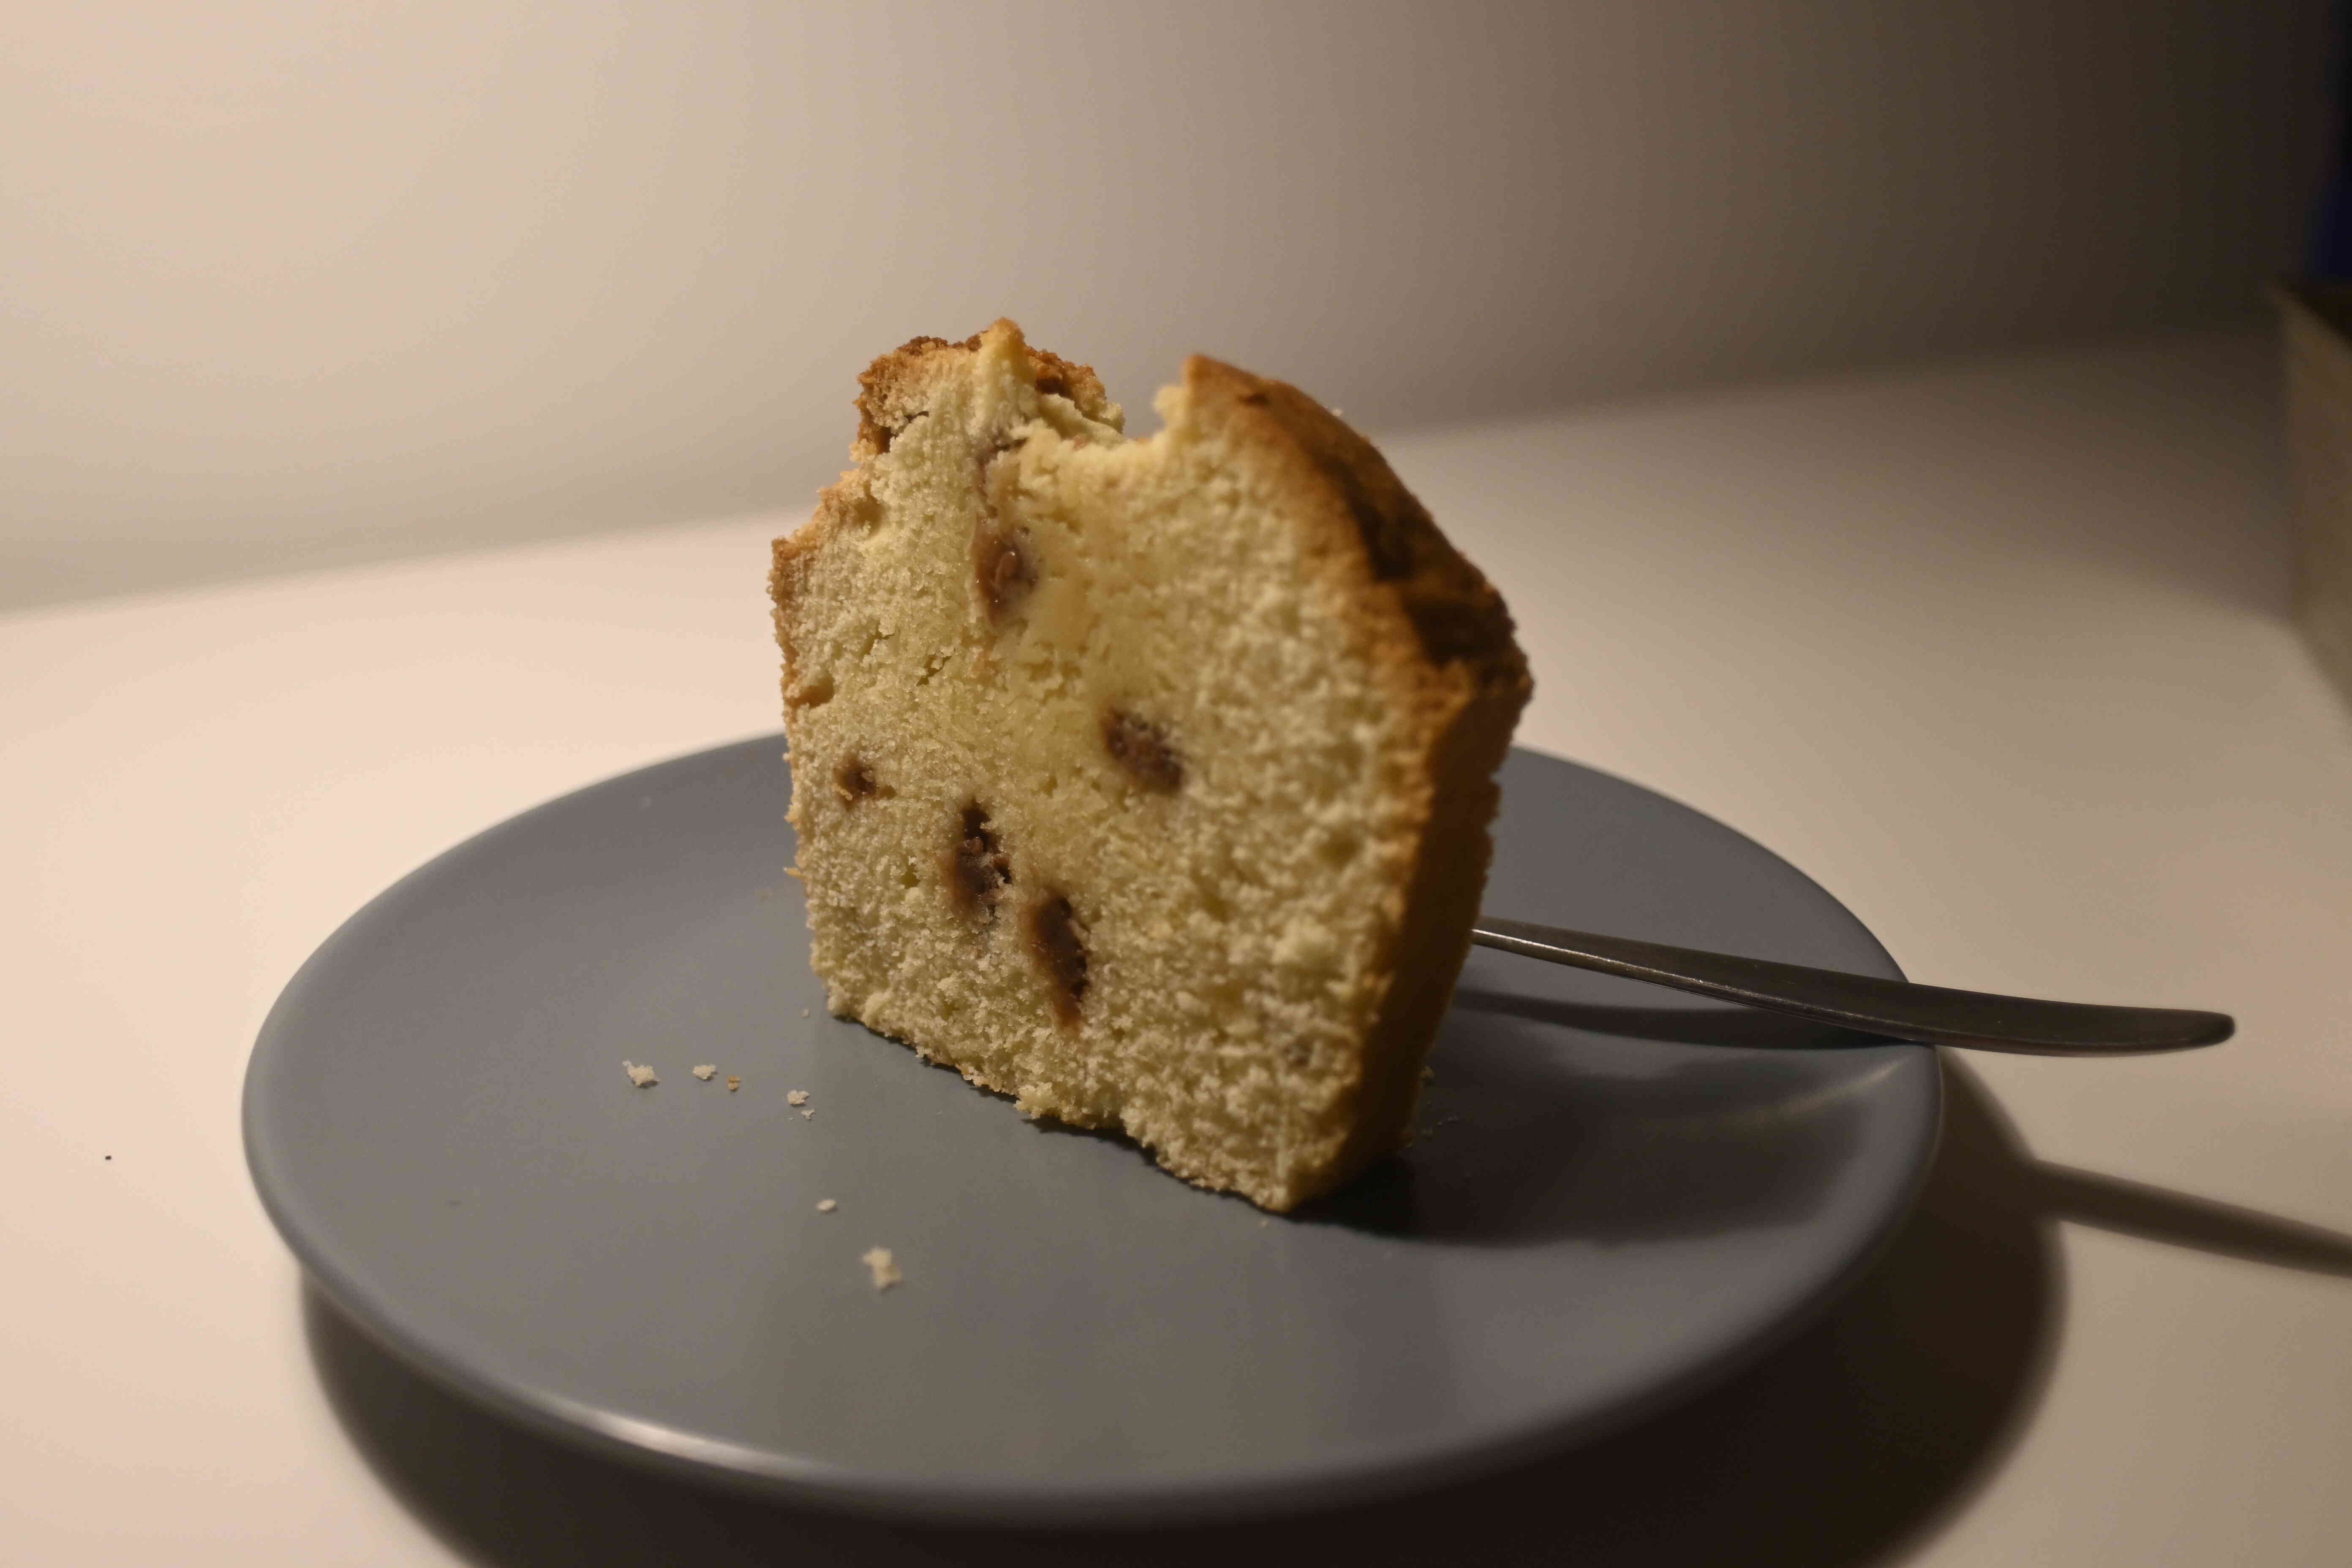
\includegraphics[height = 5cm]{media/ruehrkuchen_2.JPG}	\\
									&	\\
			\textbf{Beschreibung}	&	Der einfachste Kuchen, den man backen kann! Super variabel!\\
									&	\\
			\begin{tabular}[t]{rr}
				\textbf{Zutaten}	\\
				Für 1,5 kg 			\\
				Für 10 Portionen	\\
			\end{tabular}			&	\begin{tabular}[t]{llll}
											500 g & Weizenmehl, 550er \\
											6 & Eier \\
											250 g & Butter, weich \\
											250 g & Zucker \\
											1 TL & Backpulver \\
											1 Prise & Salz \\
											Milch, nach belieben \\								
										\end{tabular}	\\
									&	\\
			\textbf{Variationen}	&	\begin{itemize}[nosep]
											\item mit Schokodrops, Blaubeeren, Rosinen
											\item mit Kakao für Schokokuchen
											\item mit Zitronensaft getränkt und Zuckerguss
										\end{itemize}	\\
			%						&	\\	
			%\textbf{Passendes}		&	\begin{itemize}[nosep]
			%								\item ...
			%							\end{itemize}	\\
									&	\\
			\end{tabularx}
			\newpage

		\begin{tabularx}{\textwidth}{r|L}
									

			\begin{tabular}[t]{rr}
				\textbf{Zubereitung}	\\
				Vorbereitungszeit: 15 min	\\
				Backzeit:	45-60 min		\\
				Backtemperatur: 200°C \\
			\end{tabular}			&	\begin{enumerate}[nosep]
											\item Gibt die weiche Butter und den Zucker in eine Teigschüssel und verrühre es gleichmäßig.
											\item Füge die Eier hinzu, mixe das Backpulver unter das Mehl und gib alles in die Teigschüssel und verrühre es.
											\item Falls die Konsistenz etwas flüssiger sein soll füge Milch hinzu.
											\item Alle optionalen Variation vom Hauptrezept müssen jetzt hinzugefügt werden.
											\item Fette eine Teigform und gibt den Teig hinein, wobei eine Füllhöher über ~7cm zu evtl. rohen Stellen im Kuchen führen kann!
											\item Backe den Kuchen so lange bis er braun und innen möglich gut durch ist. Das kann mit einem sauberen Messer was in den Kuchen gestochen wird überprüft werden. Bleibt Teig kleben, ist es noch roh innen!
										\end{enumerate}	\\
		\end{tabularx}
		\newpage


		% Bananenbrot

		\subsection{Bananenbrot}	\label{bananenbrot}

		\begin{tabularx}{\textwidth}{r|L}
			%						& 	\includegraphics[height = 5cm]{media/vorlage.jpg}	\\
			%						&	\\
			\textbf{Beschreibung}	&	...\\
									&	\\
			\begin{tabular}[t]{rr}
				\textbf{Zutaten}	\\
				Für ... g 			\\
				Für ... Portionen	\\
			\end{tabular}			&	\begin{tabular}[t]{llll}
											... g & ... \\								
										\end{tabular}	\\
									&	\\
			\textbf{Variationen}	&	\begin{itemize}[nosep]
											\item ...
										\end{itemize}	\\
									&	\\	
			\textbf{Passendes}		&	\begin{itemize}[nosep]
											\item ...
										\end{itemize}	\\
									&	\\	
		%\end{tabularx}
		%		\newpage
		%\begin{tabularx}{\textwidth}{r|L}

			\begin{tabular}[t]{rr}
				\textbf{Zubereitung}	\\
				Vorbereitungszeit: ...	\\
				Garzeit:	...		\\
			\end{tabular}			&	\begin{enumerate}[nosep]
											\item ...
										\end{enumerate}	\\
		\end{tabularx}
		\newpage

		

		% Rezept für Kürbisbrot

		\subsection{Kürbisbrot}

		% hier sollte noch ein Bild hinein

		\begin{tabularx}{\textwidth}{r|L}
									&	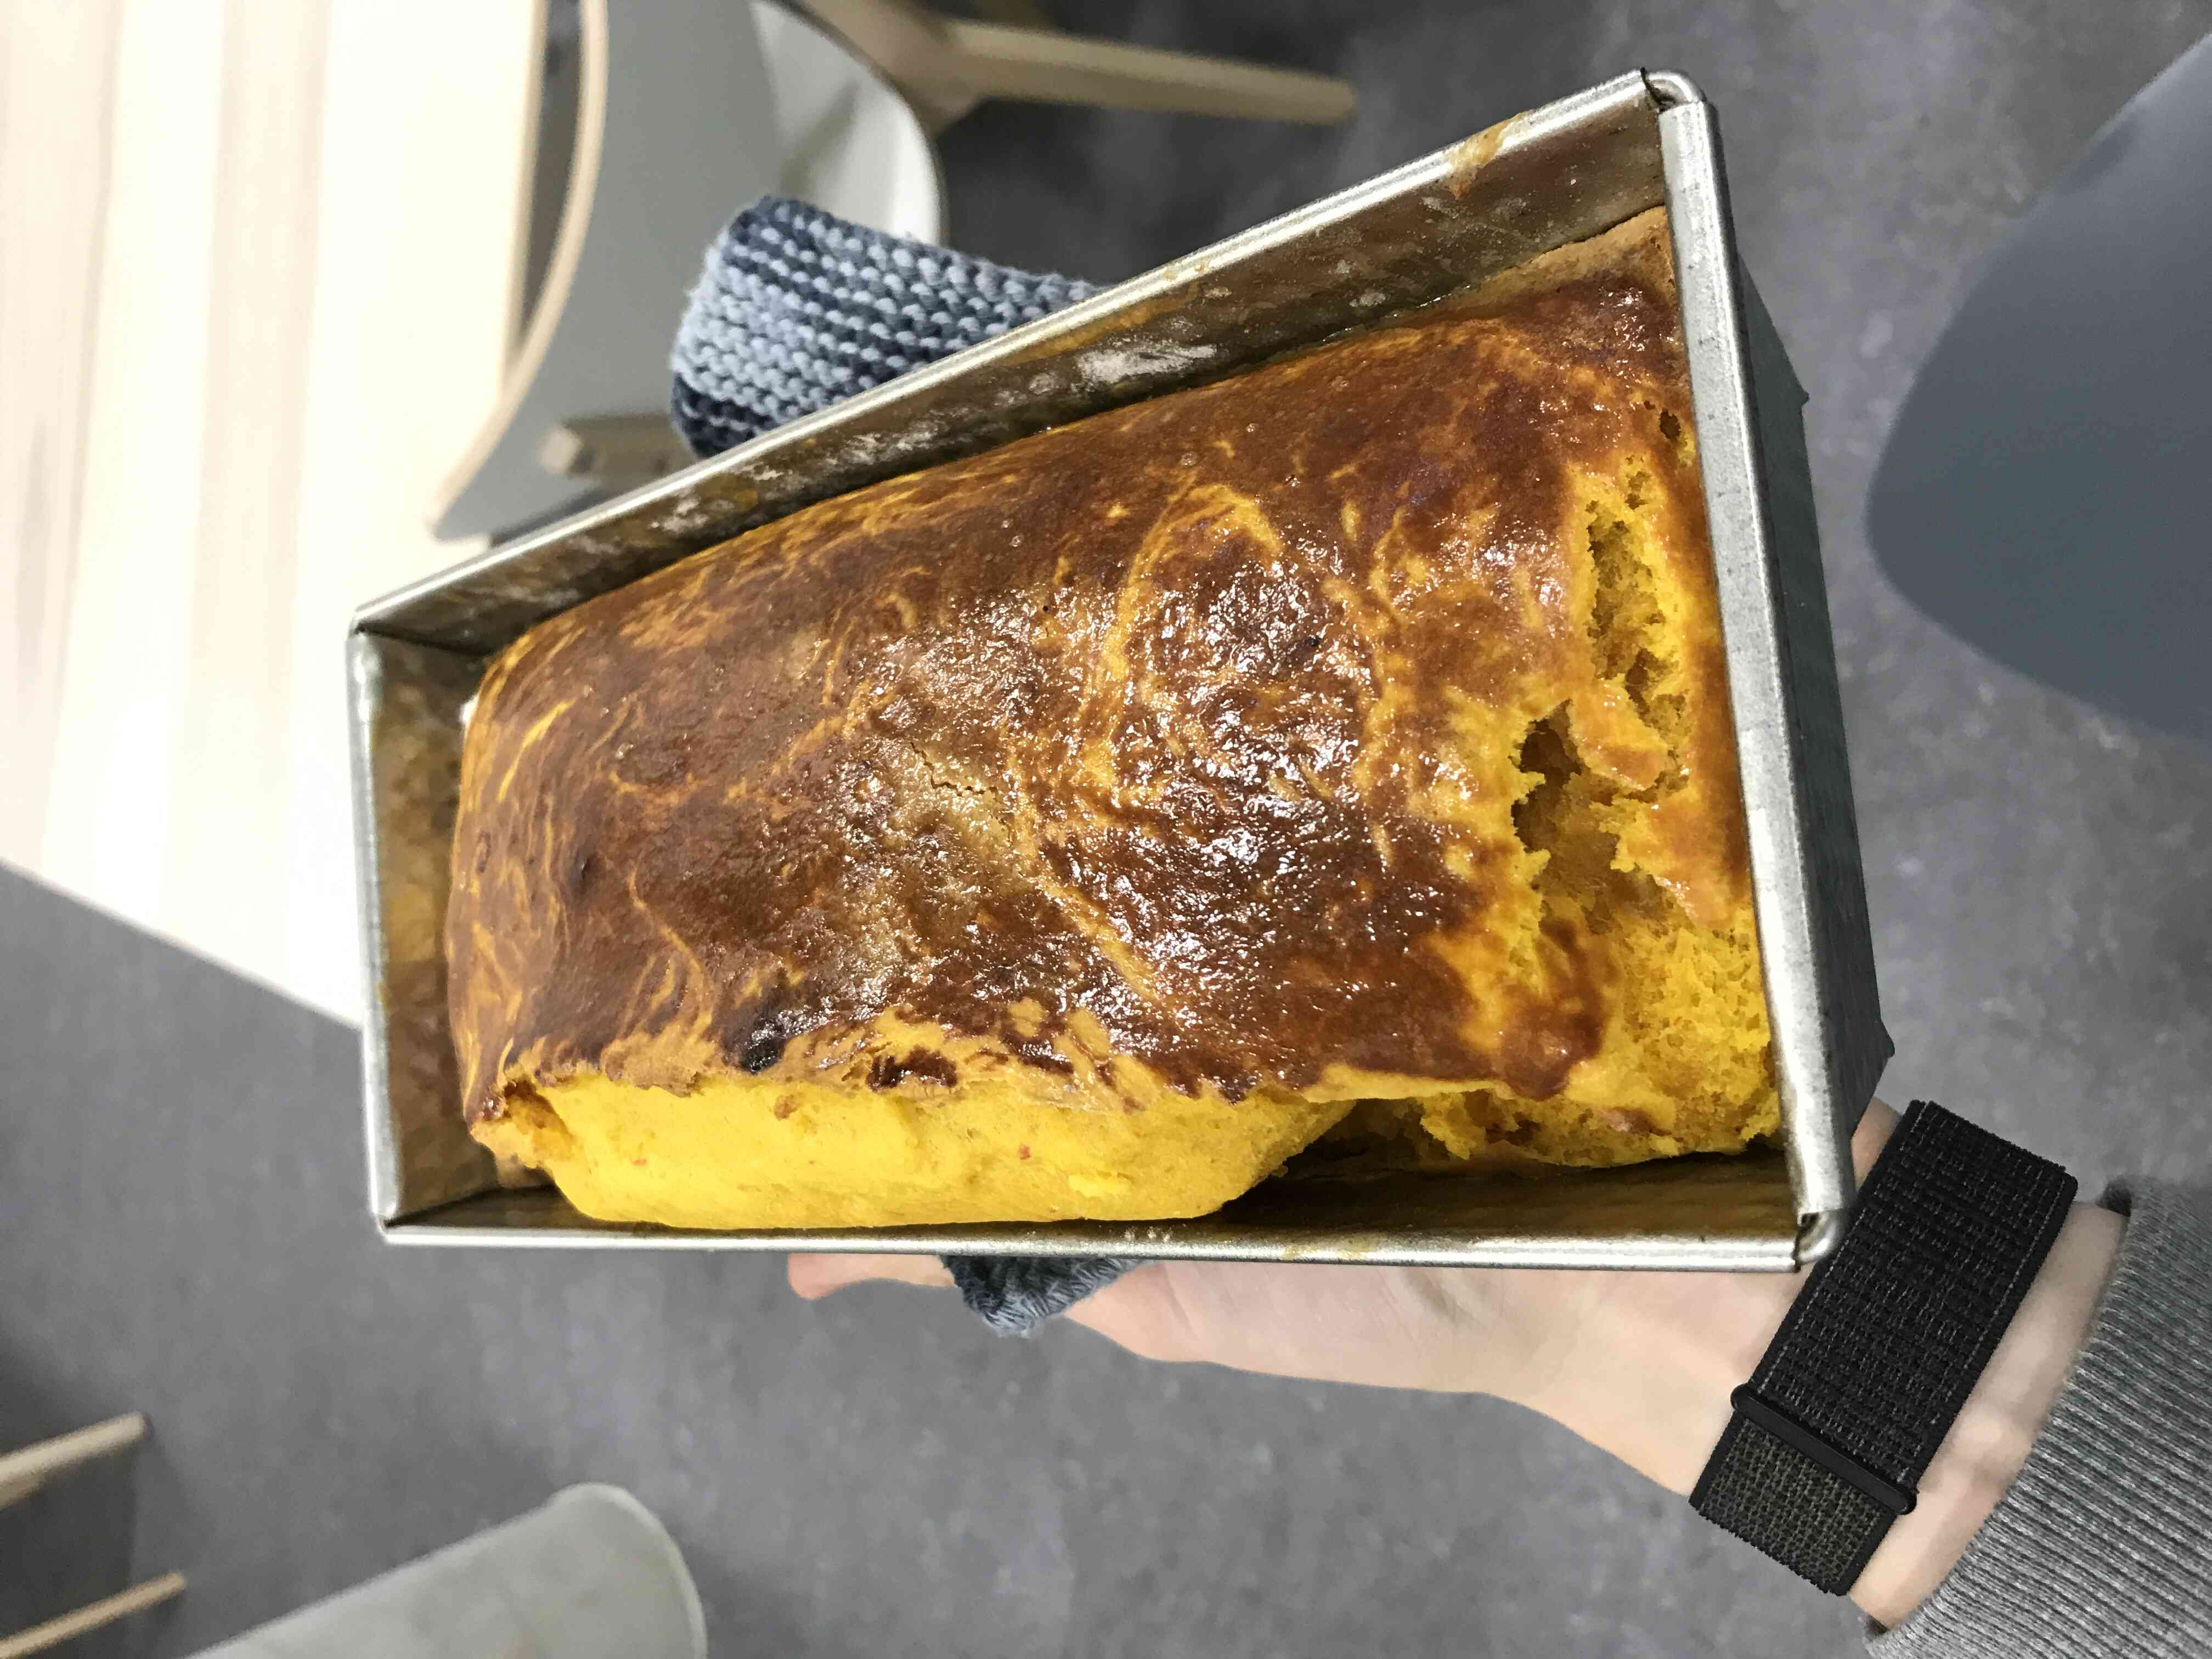
\includegraphics[height = 5cm, angle = 270]{media/kuerbisbrot.JPG}	\\
									&	\\
			\textbf{Beschreibung}	&	Ein herbstliches Gebäck, welches eine Abwandlung des Brioche darstellt.\\
									&	\\
			\begin{tabular}[t]{rr}
				\textbf{Zutaten}	\\
				Für 700 g Teig		\\
			\end{tabular}			&	\begin{tabular}[t]{ll}
											500 g	&	Weizenmehl 550er \\
											250 g	&	Wasser \\
											150 g	&	Kürbispürree \\
											80 g	&	Butter \\
											100 g	&	Zucker \\
											1 		&	Ei \\
											4 g		&	Salz \\
											1-3 g	&	Trockenhefe									
										\end{tabular}	\\
									&	\\
			\textbf{Variationen}	&	\begin{itemize}[nosep]
											\item
										\end{itemize}	\\
									&	\\	
			\textbf{Passendes}		&	\begin{itemize}[nosep]
											\item Butter drauf ;)
										\end{itemize}	\\
									&	\\	
			\begin{tabular}[t]{rr}
				\textbf{Zubereitung}	\\
				Arbeitszeit: 	\\
				Gesamtzeit:		\\
			\end{tabular}			&	\begin{enumerate}[nosep]
											\item
										\end{enumerate}	\\
		\end{tabularx}
		\newpage

		% Zupfkuchen

		\subsection{Zupfkuchen}

		\begin{tabularx}{\textwidth}{r|L}
									& 	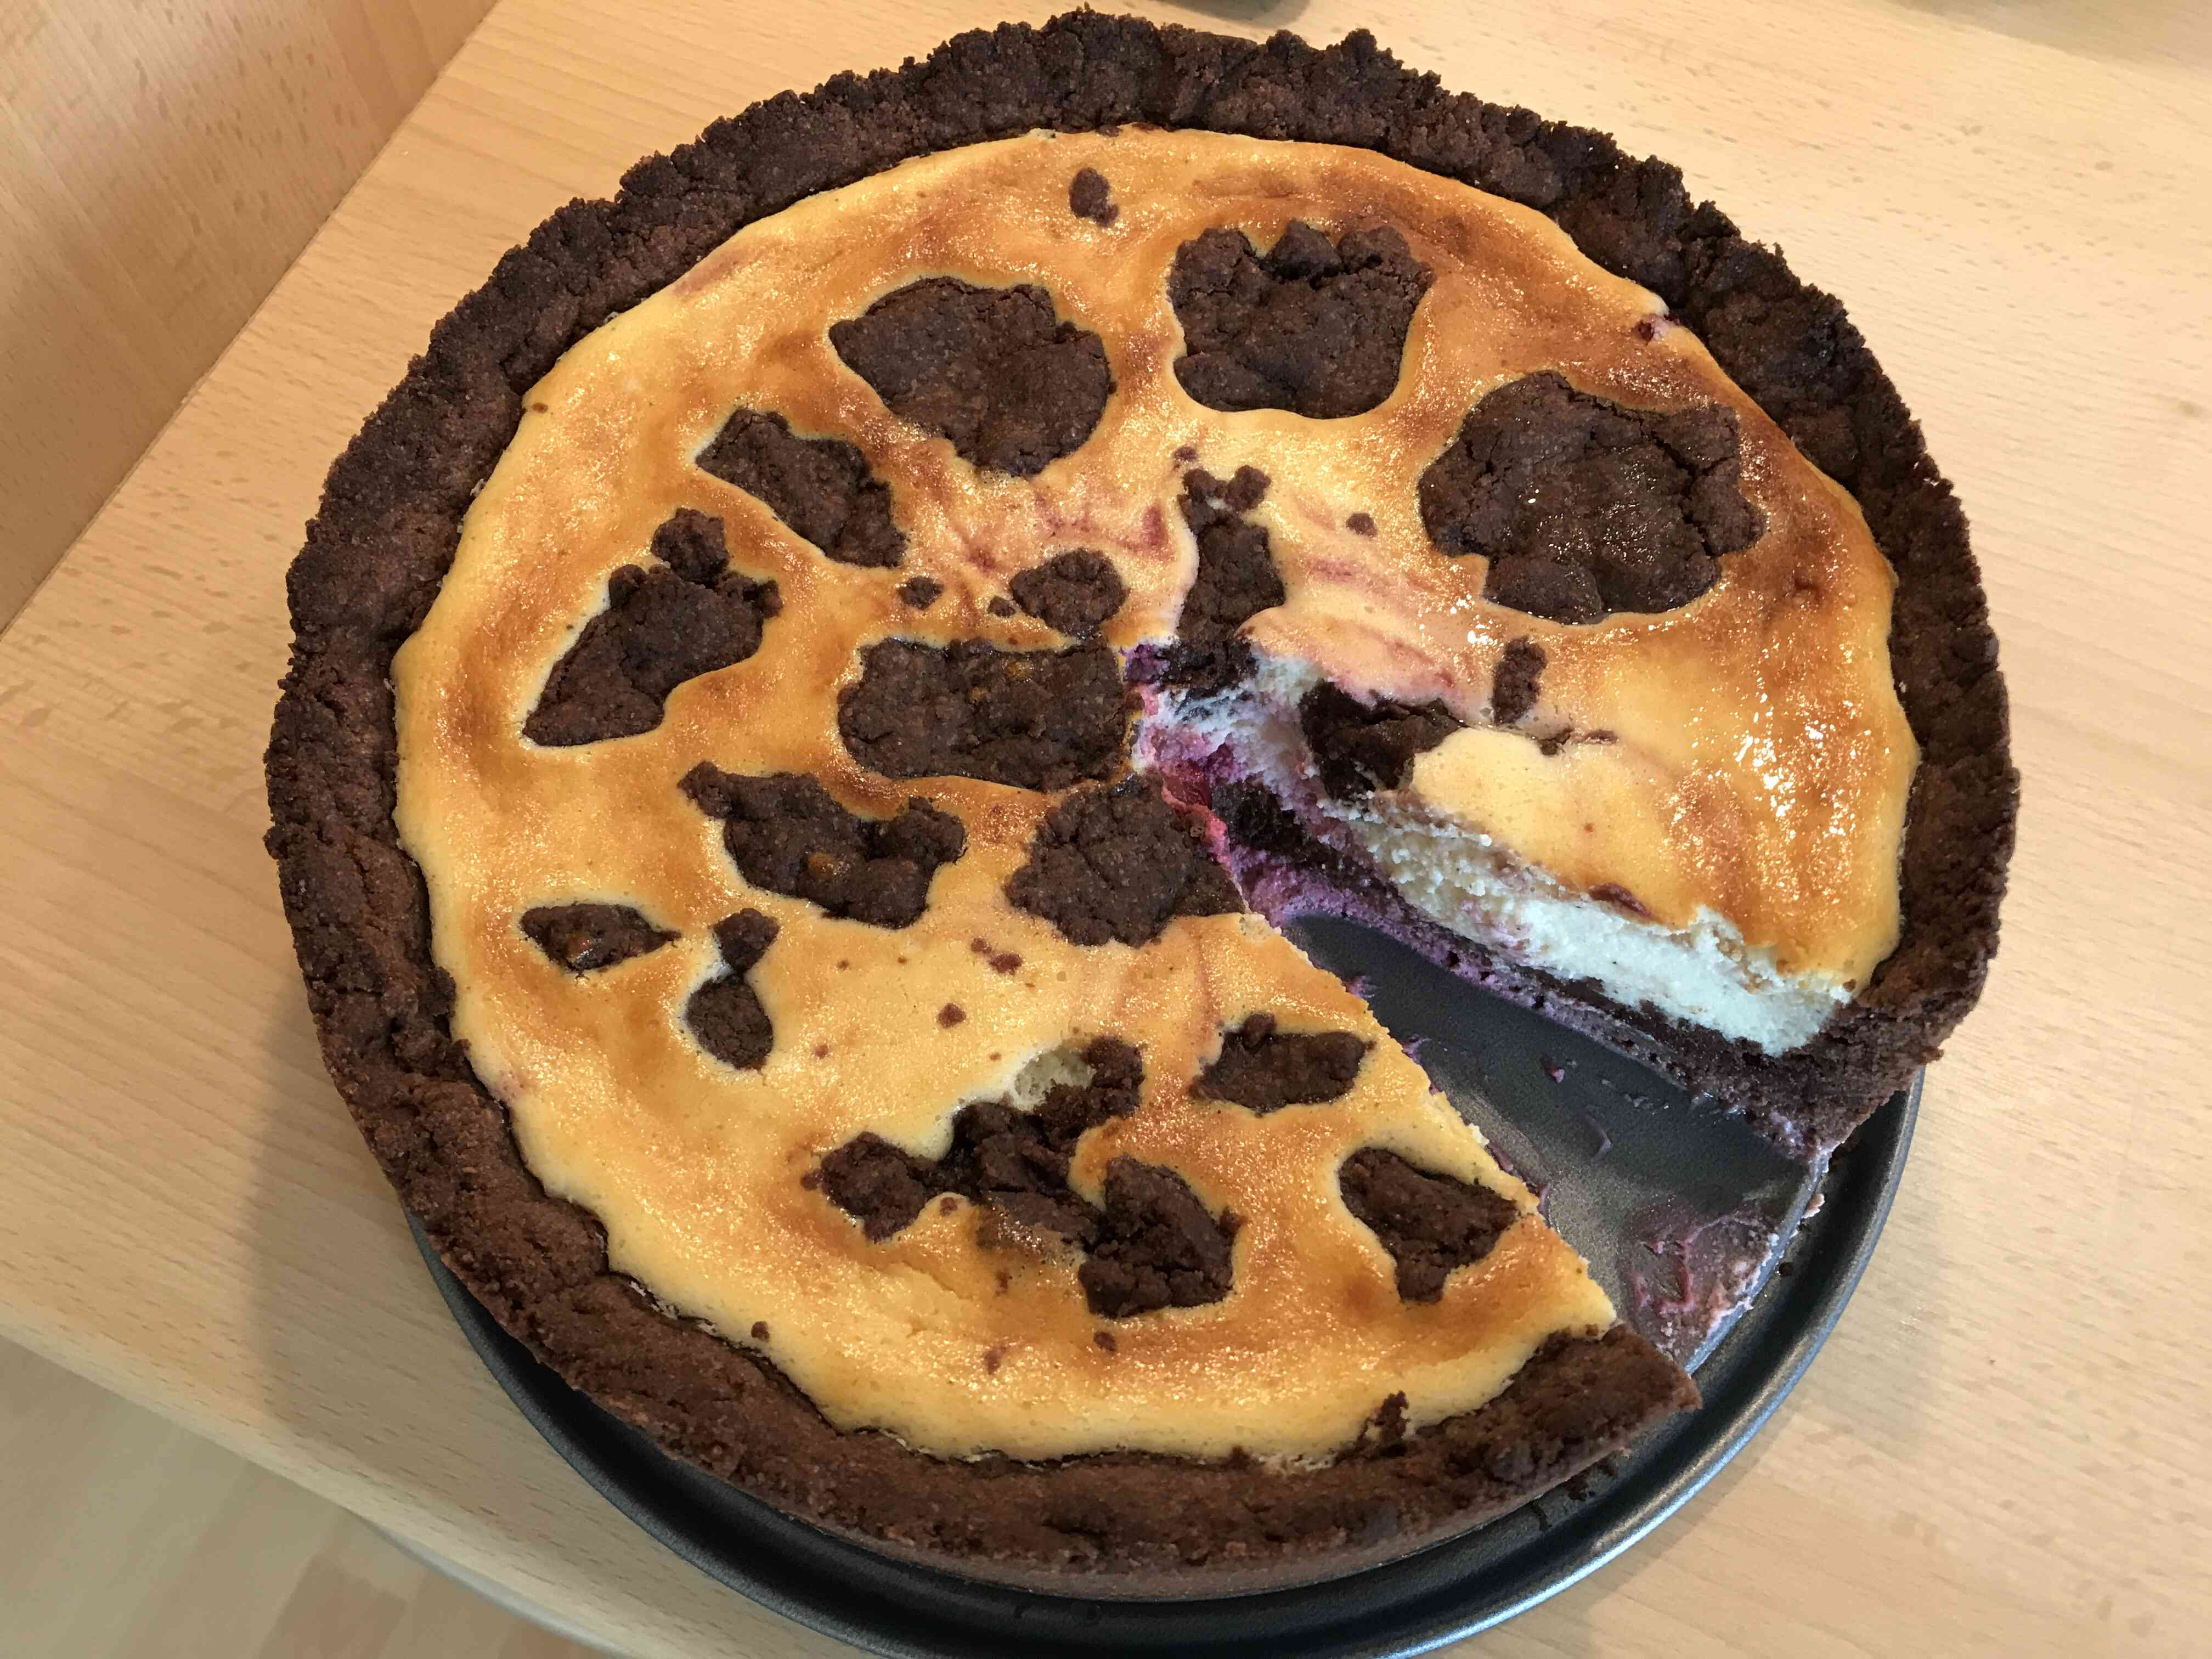
\includegraphics[height = 5cm]{media/zupfkuche.JPG}	\\
									& \\
			\textbf{Beschreibung}	&	Ein zwar nicht besonders traditionell wertvoller Kuchen, aber dafür eine gelungene schokoladige Abwechslung zum normalen Käsekuchen!\\
									&	\\
			\begin{tabular}[t]{rr}
				\textbf{Zutaten}	\\
				Für 2 kg 			\\
				Für 8-12 Portionen	\\
			\end{tabular}			&	\begin{tabular}[t]{llll}
											Kakao-Boden \\
												& 500 g & Weizenmehl 550er \\
												& 250 g & Butter \\
												& 200 g & Zucker \\
												& 50 g	& Kakao \\
												& 3 TL & Backpulver \\	
												& 1 & Ei \\
											Füllung \\
												& 500 g & Quark \\
												& 200 g & Zucker \\
												& 250 g & Butter/Öl \\
												& 3 &	Eier \\
												& 40 g & Stärke \\
										\end{tabular}	\\
									&	\\	
			\begin{tabular}[t]{rr}
				\textbf{Zubereitung}	\\
				Springform 23 cm	\\
				Backtemperatur: 200°C	\\
				Backzeit: 40-45 min	\\
				Abkühlen: mind. 1h \\
				(ansonsten Matsch!)\\
			\end{tabular}			&	\begin{enumerate}[nosep]
											\item Vermische die Zutaten für den Kakao-Boden in einer Schüssel, bis sich ein gleichmäßiger Teig bildet.
											\item Lege 2/3 des Teiges gleichmäßig in die Springform.
											\item Rühre die Füllung an und gib sie in die Springform.
											\item Gib nun die den restlichen Kakao-Teig in gezupfter Form auf die Füllung und backe den Kuchen.
										\end{enumerate}	\\
		\end{tabularx}
		\newpage




		% Brownies

		\subsection{Brownies}

		\begin{tabularx}{\textwidth}{r|L}
									& 	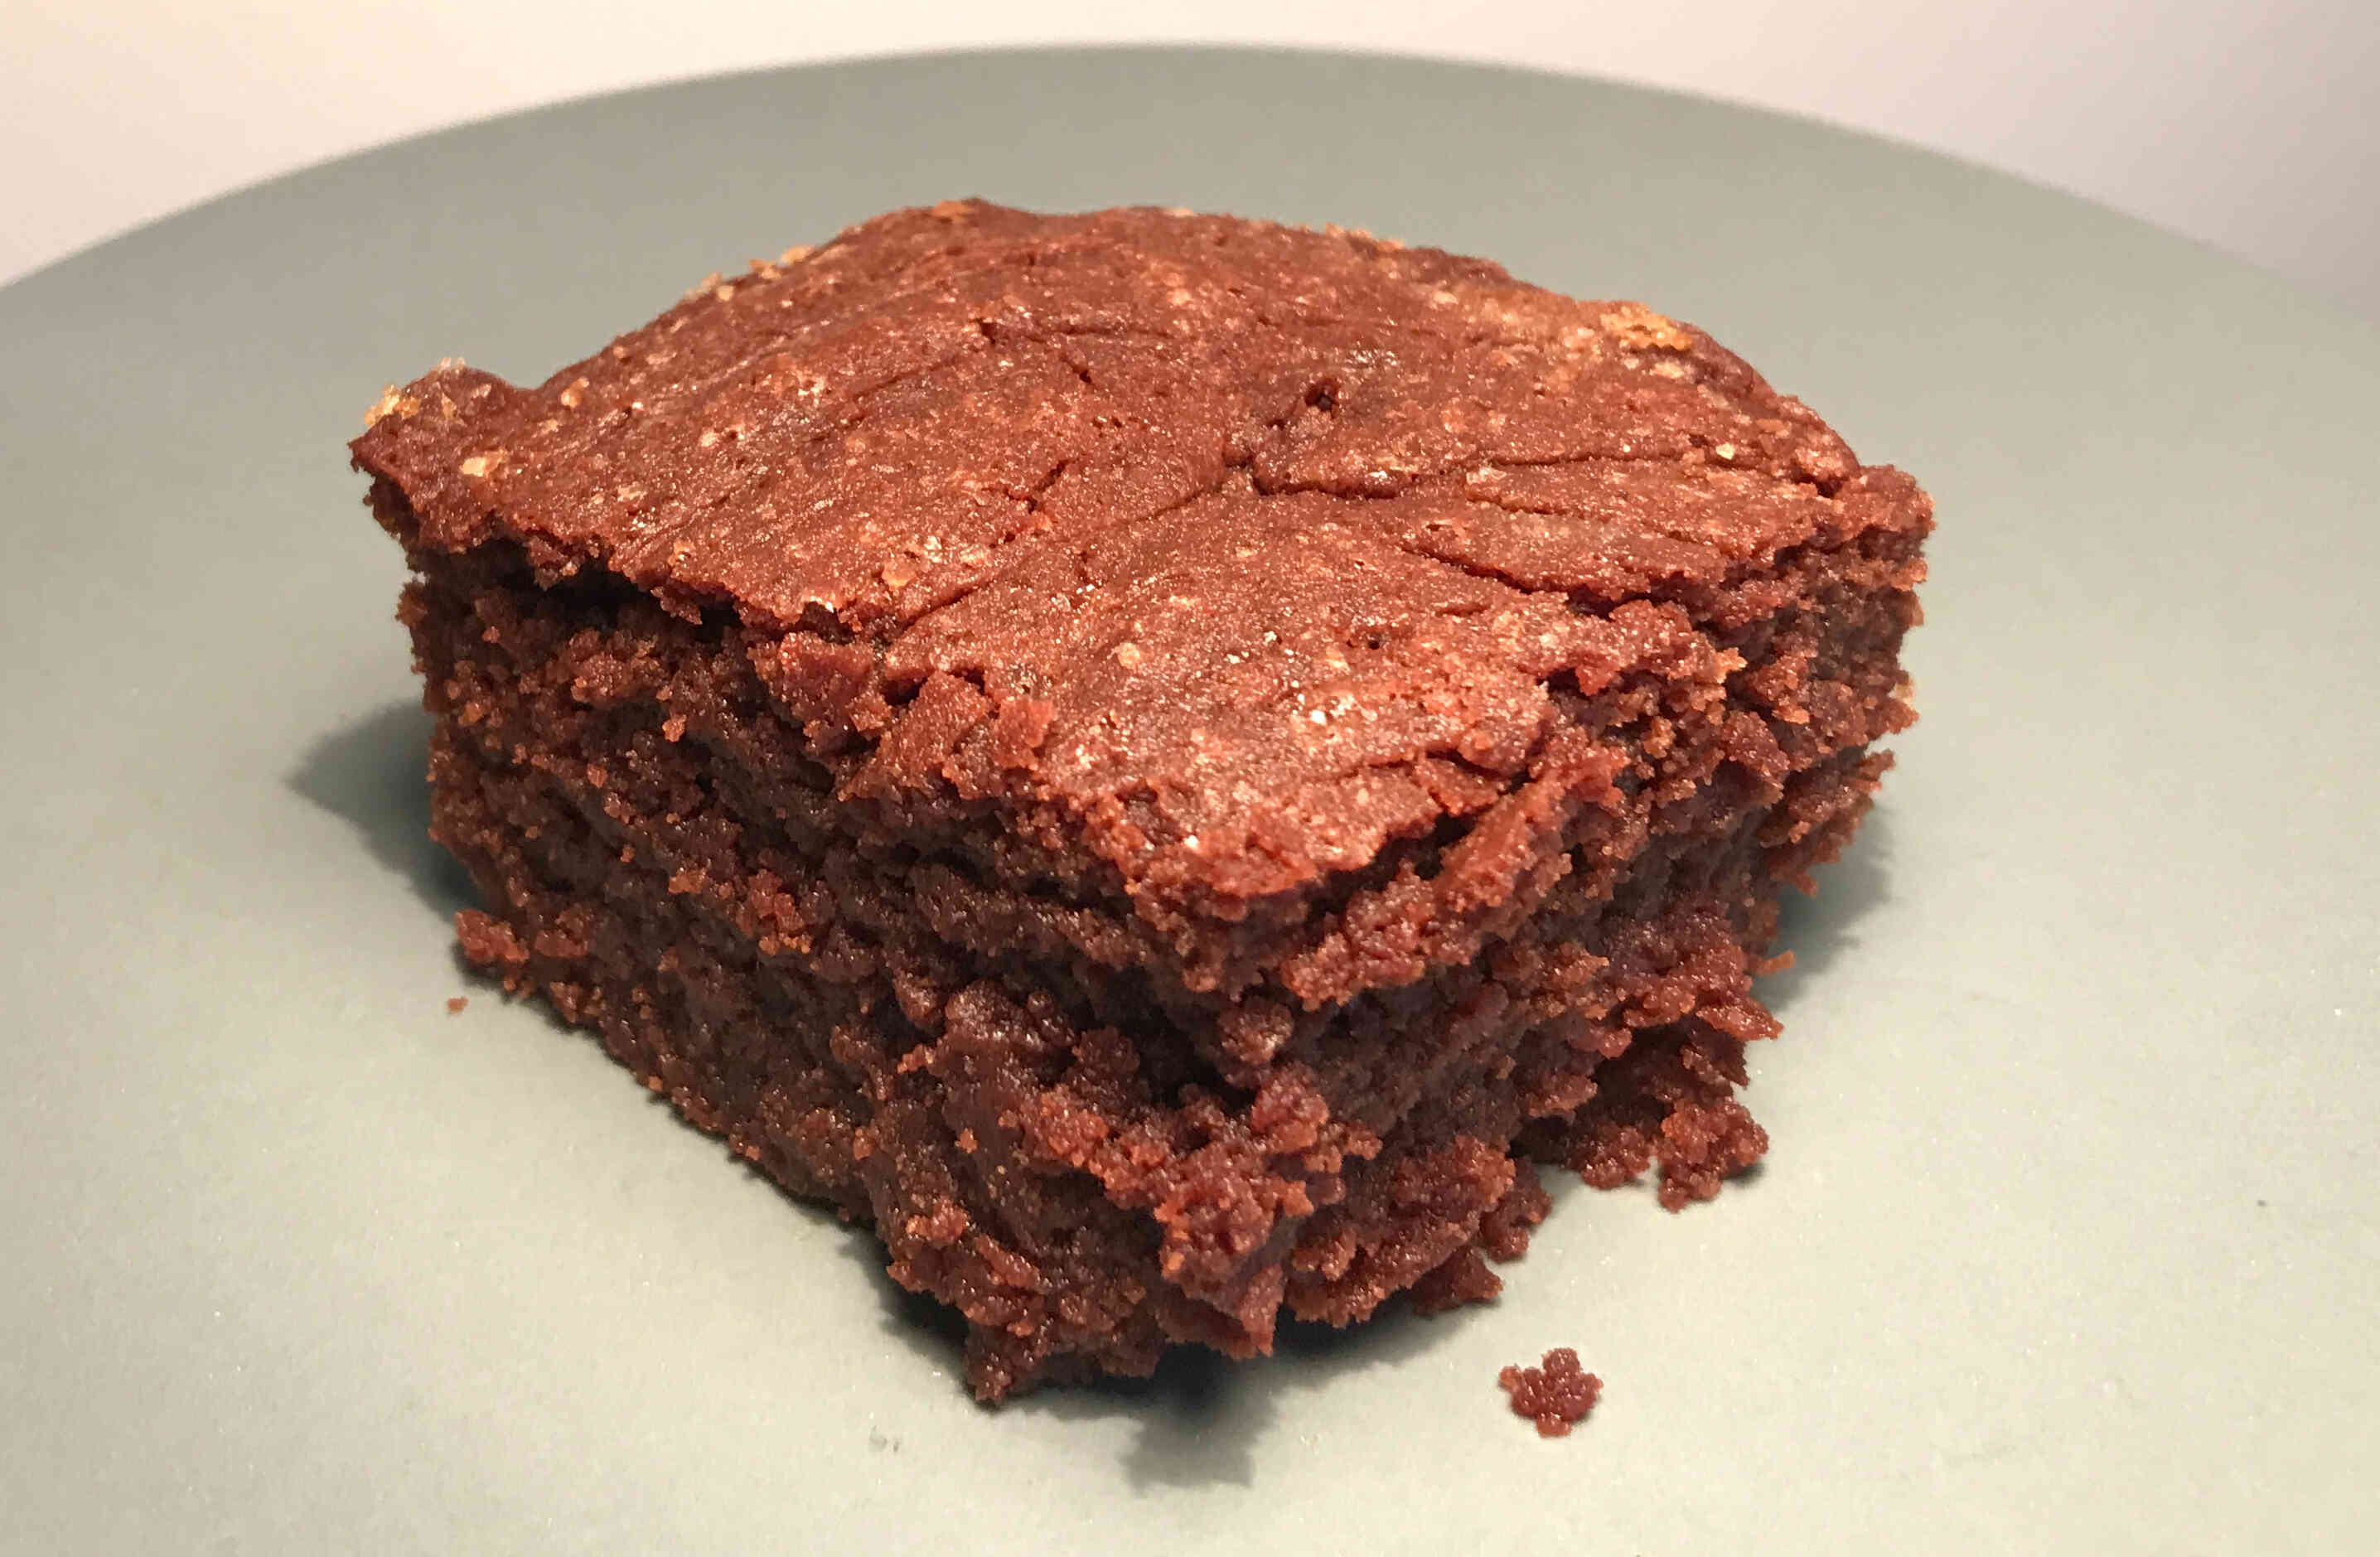
\includegraphics[height = 5cm]{media/brownie.JPG}	\\
									&	\\
			\textbf{Beschreibung}	&	Eine schokoladige Sünde...\\
									&	\\
			\begin{tabular}[t]{rr}
				\textbf{Zutaten}	\\
				Für 1,7 kg 			\\
				Für 20 Portionen	\\
			\end{tabular}			&	\begin{tabular}[t]{llll}
											300 g & Schokolade, zartbitter \\
											400 g & Zucker 	\\
											250 g & Butter	\\
											150 g & Mehl	\\
											5	  & Eier \\
											10 g  & Salz \\
											Vanille
										\end{tabular}	\\
									&	\\
			\textbf{Variationen}	&	\begin{itemize}[nosep]
											\item ...
										\end{itemize}	\\
									&	\\	
			\textbf{Passendes}		&	\begin{itemize}[nosep]
											\item ...
										\end{itemize}	\\
									&	\\	
			\begin{tabular}[t]{rr}
				\textbf{Zubereitung}	\\
				Arbeitszeit: 15 min	\\
				Gesamtzeit:	1 h		\\
				Backtemperatur: 180°C	\\
				Backzeit: 45 min \\
				\emph{Achtung! Muss gar sein!}	\\
			\end{tabular}			&	\begin{enumerate}[nosep]
											\item Mehl und Salz in einer Schüssel verrühren
											\item Schokolade, Butter in einem Topf langsam erhitzen
											\item Zucker in die geschmolzenen Zutaten geben und gleichmäßig verrühren
											\item Eier zu der Masse hinzugeben, wobei kein Mixer verwendet werden soll
											\item Letztendlich das Mehl und Salz hinzugeben
											\item Teig in eine Backform geben und backen
											\item vollständig abkühlen lassen
										\end{enumerate}	\\
		\end{tabularx}
		\newpage

		%Pi-Day Pi! oder auch Apple-Pi

		\subsection{Gedeckte Apple-Pie ($\pi$-Day-Pie)}

		\begin{tabularx}{\textwidth}{r|L}
									& 	
\includegraphics[height = 5cm]{media/apple_pi.JPG}	\\
									&	\\
			\textbf{Beschreibung}	&	Ein amerikanische oder britische Erfindungen, bei der irgendeine herzhafte oder süße Füllung mit einer Art salzigem Mürbeteig ummantelt wird. Auf Deutsch muss sie den unwürdigen Namen „Pastete“ trage.\\	
									&	Der perfekte Pie für den höchsten Feiertag eines Naturwissenschaftlers, den $\pi$-Day!\\
									&	\\
			\begin{tabular}[t]{rr}
				\textbf{Zutaten}	\\
				Für 1,6 kg 			\\
				Für 16 Portionen	\\
			\end{tabular}			&	\begin{tabular}[t]{llll}
											Boden und Deckel: \\
											\begin{tabular}{lll}
												400 g & Weizenmehl, 550er \\
												250 g & Butter, möglichst kühl \\
												13 g & Salz \\
												60 g & Zucker \\
												100 g & Wasser \\
											\end{tabular} \\
											Apfel-Füllung: \\
											\begin{tabular}{ll}
												800 g / 5 Stück & Äpfel \\
												140 g & Zucker \\
												40 g & Mehl \\
												1/2 TL & Zimt \\
												Salz \\
												evtl. Ei & (zum Bestreichen) \\
											\end{tabular}								
										\end{tabular}	\\
									&	\\
	%		\textbf{Variationen}	&	\begin{itemize}[nosep]
	%										\item ...
	%									\end{itemize}	\\
	%								&	\\	
			\textbf{Passendes}		&	\begin{itemize}[nosep]
											\item Vanillesoße
											\item Schlagsahne
										\end{itemize}	\\
									&	\\
		\end{tabularx}
		
		\begin{tabularx}{\textwidth}{r|L}
			\begin{tabular}[t]{rr}
				\textbf{Zubereitung}	\\
				Arbeitszeit: ...	\\
				Backtemperatur: 180°C \\
				Backzeit: 45-60 min \\
			\end{tabular}			&	\begin{enumerate}[nosep]
											\item Gib Mehl, Zucker, Salz in eine Schüssel, schneide die kalte Butter in kleine Würfel, damit sie besser verknetet werden kann und vermenge alles mit einem Stampfwerkzeug. Dabei soll die Butter möglichst nicht schmelzen, also sind die Hände eher ungeeignet.
											\item Füge nun nach und nach so viel Wasser hinzu, bis eine gute Konsistenz für die Verarbeitung vorhanden ist.
											\item Forme eine Kugel und lasse alles für 30-60 min im Kühlschrank liegen.
											\item Schneide die Äpfel in kleine Stücke und vermische sie mit dem Zucker, Mehl, Salz, Muskat und Zimt.
											\item Teile den Teig in 2/3 für den Boden und 2/3 für den Deckel auf und rolle beide möglichst rund aus, sodass die Backform ausgekleidet werden kann. Achte auf kühle Hände!
											\item Schneide in den Deckel ein beliebiges Muster. Pi ist gewünscht, andere naturwissenschaftliche Symbole sind aber auch erlaubt.
											\item Gib den Boden in die Form, dann die Füllung und schließe alles mit dem Deckel. Dieser sollte am Rand am besten noch ein wenig mit dem Boden verformt werden, um einen guten Abschluss hinzubekommen.
											\item Backe die Apple Pie bei 180°C für 30 min, bis eine ordentliche Färbung zu sehen ist. 
										\end{enumerate}	\\
		\end{tabularx}
		\newpage

		% Hefezopf

		\subsection{Hefezopf}	\label{Hefezopf}

		\begin{tabularx}{\textwidth}{r|L}
									& 	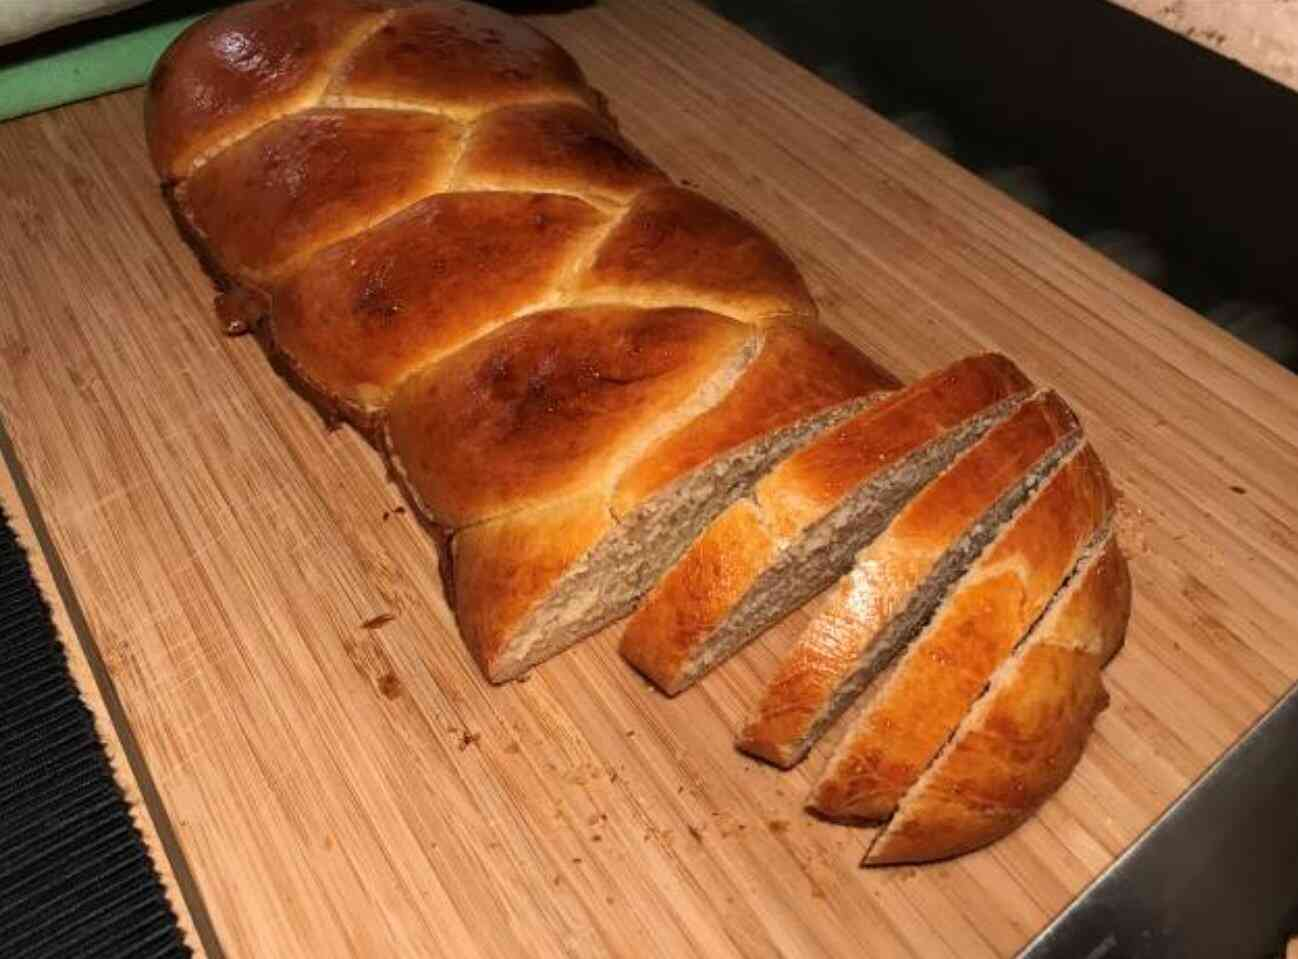
\includegraphics[height = 5cm]{media/hefezopf.jpg}	\\
									&	\\
			\textbf{Beschreibung}	&	Ein tolles Gebäck für ein Ostern mit viel gutem Essen.\\
									&	\\
			\begin{tabular}[t]{rr}
				\textbf{Zutaten}	\\
				Für ca. 900 g 			\\
				Für 4 Portionen	\\
			\end{tabular}			&	\begin{tabular}[t]{llll}
											500 g & Mehl \\	
											180 ml ?& Milch\\
											70 g & Butter \\
											100 g & Zucker \\ % geändert von 70g auf Anraten von Uta
											1 & Ei, für Teig und zum Bestreichen \\
											4 g & Salz \\
											1 g & Trockenhefe \\
										\end{tabular} \\
									&	\\	
			\textbf{Passendes}		&	\begin{itemize}[nosep]
											\item Butter
											\item Marmelade
										\end{itemize}	\\
									&	\\
		\end{tabularx}
		\newpage
		\begin{tabularx}{\textwidth}{r|L}
			\begin{tabular}[t]{rr}
				\textbf{Zubereitung}	\\
				Arbeitszeit: 20 min	\\
				Gehzeit: ca. 12 h \\
				Backtemperatur: 180 °C \\
				Backzeit: 30-40 min \\
			\end{tabular}			&	\begin{enumerate}[nosep]
											\item Löse die Hefe in der Milch in einer angemessen großen Schüssel auf.
											\item Gib das Mehl, die Butter, den Zucker, die Hälfte des Ei und das Salz hinzu und verrühre kurz alles homogen.
											\item Knete nun den Teig für 10 min ordentlich, sodass sich das Gluten gut bilden kann.
											\item Lasse den Teig ca. 12 h bei Zimmertemperatur gehen.
											\item Bringe den Teig, mit möglichst wenig Mehleinsatz, nun wieder unter Spannung und Teile ihn in drei gleich große Stücke.
											\item Rolle die Drittel, ohne die Oberflächenspannung zu mindern, in ca. 40 cm lange Stränge.
											\item Verflechte sie miteinander und verbinde sie oben und unten möglichst gut.
											\item Optional lasse den Teigling 1-3 h an einem warmen Ort ruhen, sodass er ordentlich an Größe gewinnt.
											\item Heize den Backofen auf 180°C mit Ober- und Unterhitze vor.
											\item Streiche den Teigling noch mit Milch und Ei ein und backe ihn für 30-40 min, bis die Kruste eine gute Farbe hat und der Hefezopf beim Draufklopfen hol klingt.
										\end{enumerate}	\\
		\end{tabularx}
		\newpage

		% Zimtschnecken

		\subsection{Zimtschnecken}	\label{zimtschnecken}

		\begin{tabularx}{\textwidth}{r|L}
									& 	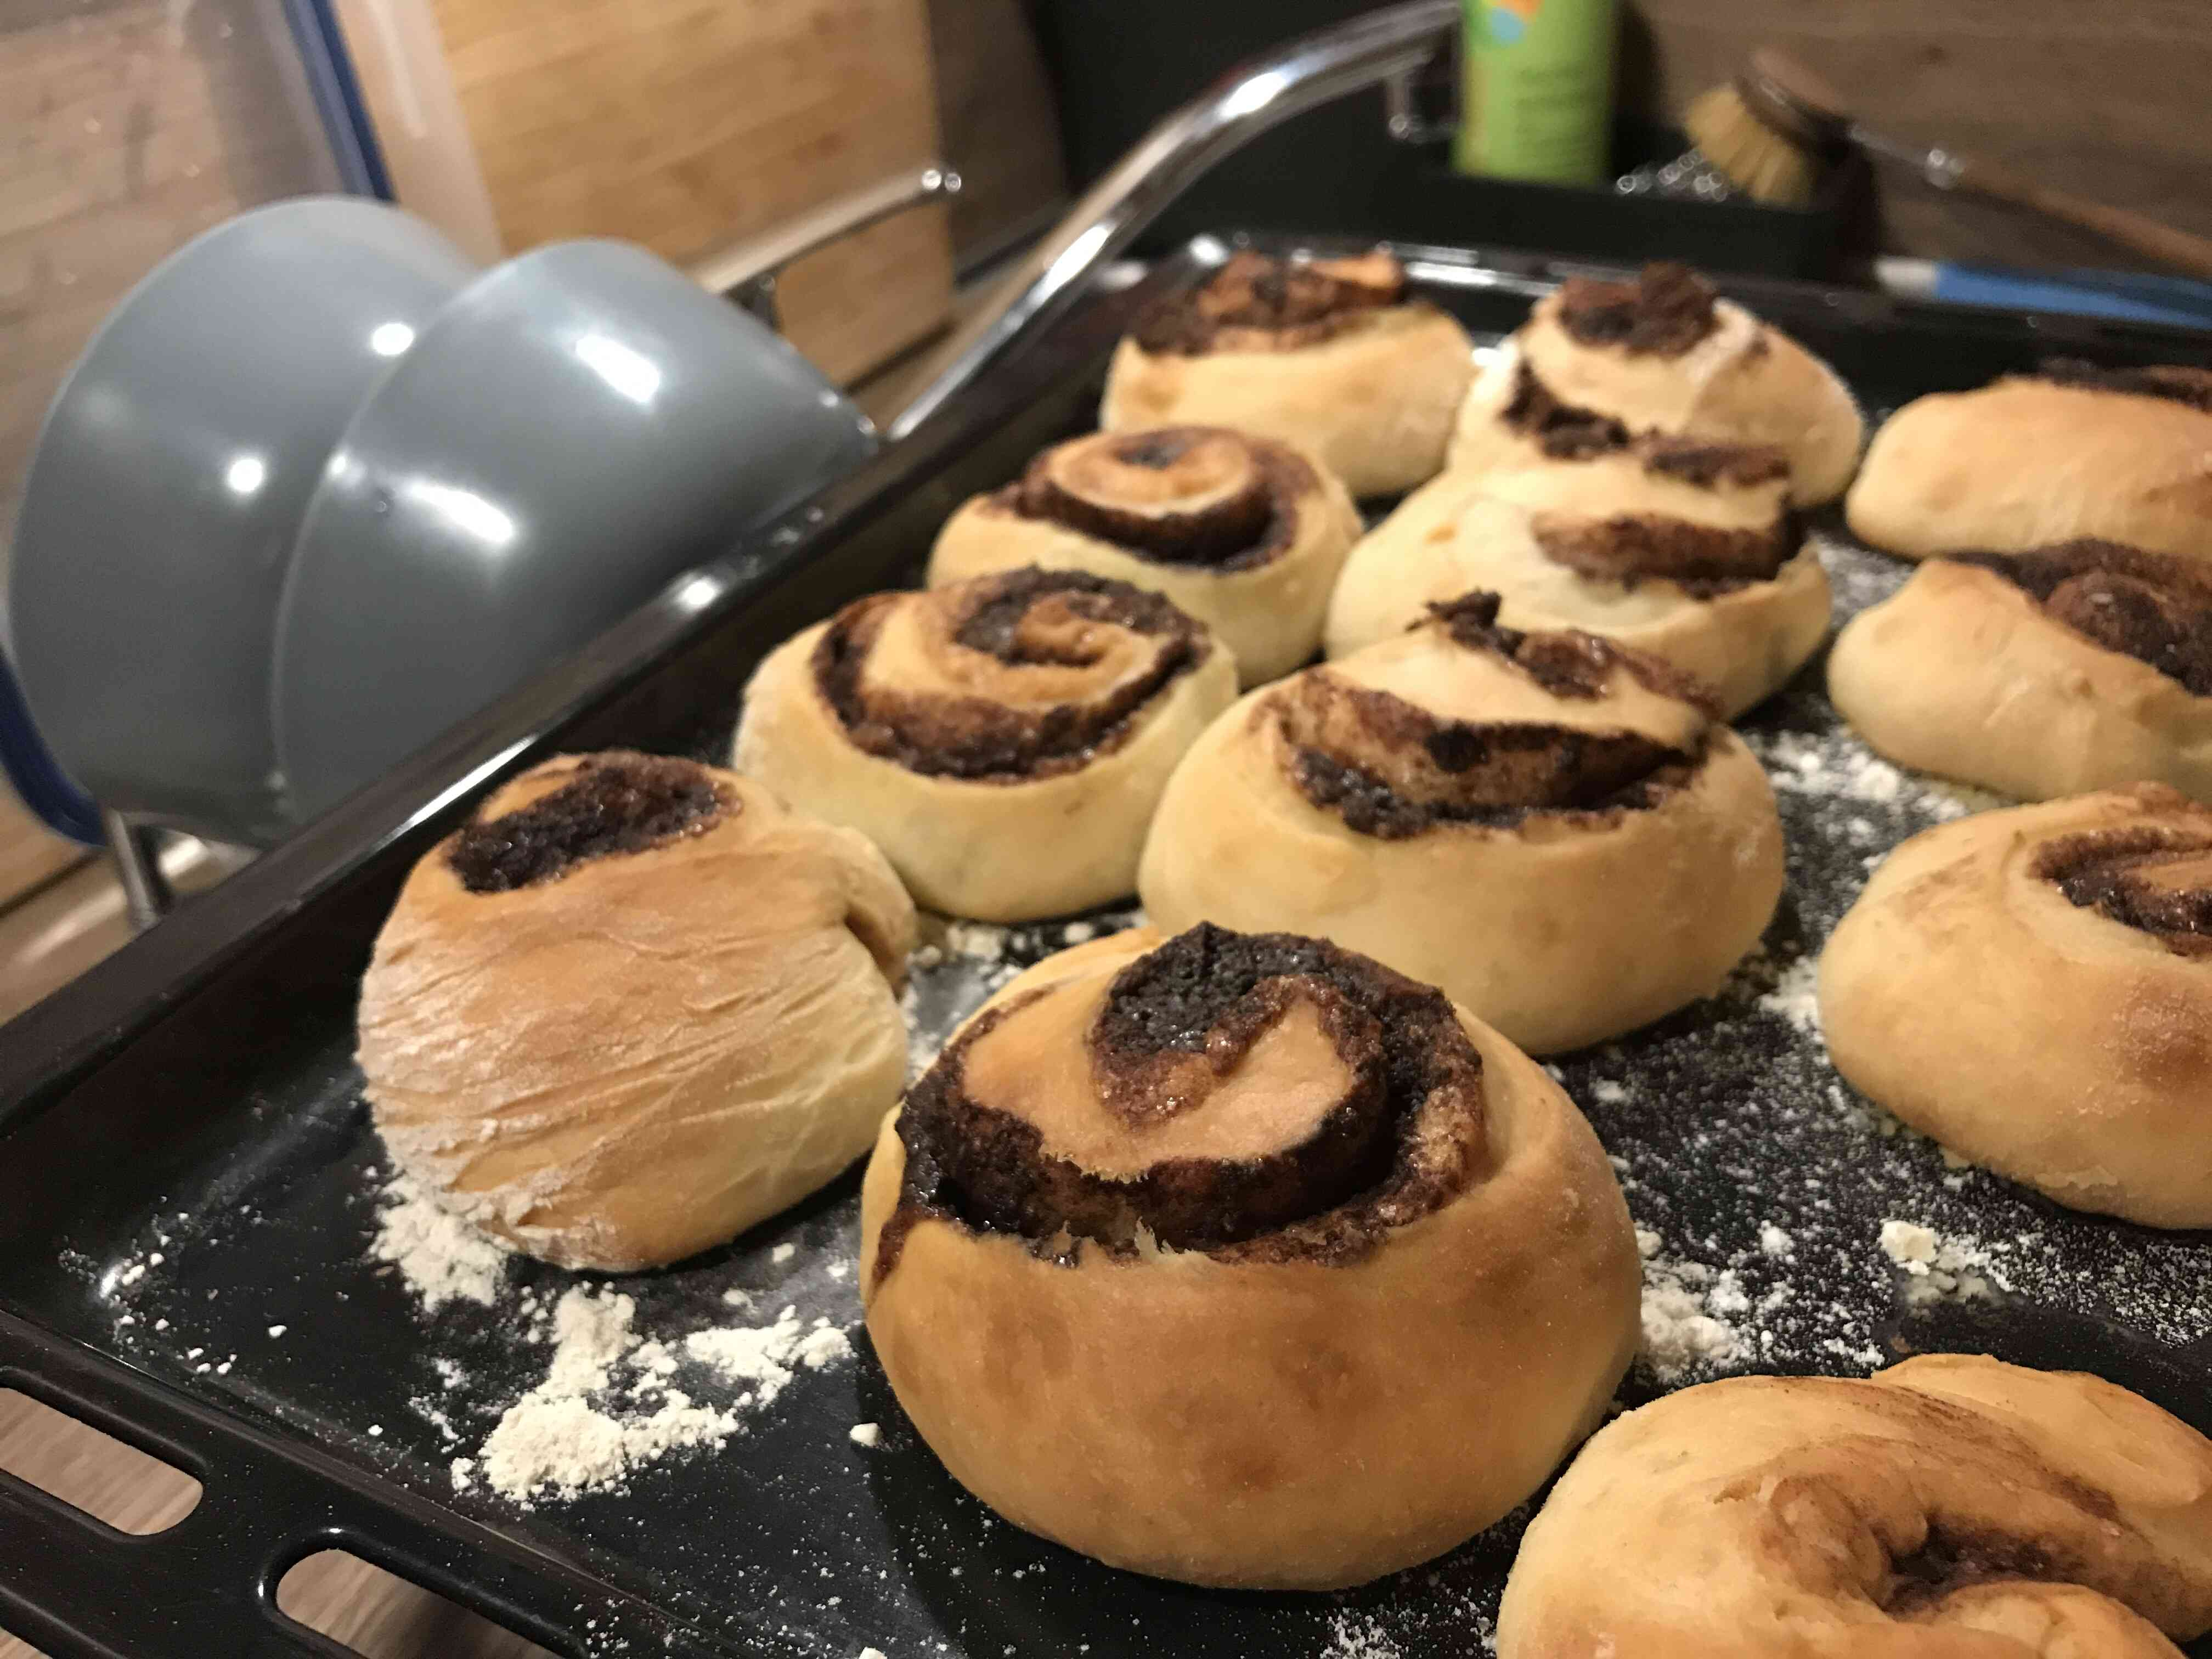
\includegraphics[height = 5cm]{media/zimtschnecken.JPG}	\\
									&	\\
			\textbf{Beschreibung}	&	Früher dachte ich, dass man gute Zimtschnecken wohl nur bei IKEA in Plastiktüten bekommen kann…\\
									&	\\
			\begin{tabular}[t]{rr}
				\textbf{Zutaten}	\\
				Für 1 kg 			\\
				Für 16 Zimtschnecken	\\
			\end{tabular}			&	\begin{tabular}[t]{llll}
											Hefeteig: \\
											& 500 g & Weizenmehl, 550er \\
											& 300 ml & Milch (Milch/Mehl = 60 \%) \\
											& 100 g & Zucker\\
											& 6 g & Salz \\
											& 75 g & Butter \\
											& 1 g & Trockenhefe \\
											Füllung: \\
											& 50 g & Butter \\
											& 100 g & Zucker \\
											& Zimt \\
											& Kardamom \\
										\end{tabular}	\\
									&	\\
			\textbf{Variationen}	&	\begin{itemize}[nosep]
											\item ...
										\end{itemize}	\\
									&	\\	
			\textbf{Passendes}		&	\begin{itemize}[nosep]
											\item Vanillesoße \ref{vanillesosse}
											\item Frosting aus Sahne, Zucker, Salz, Butter
										\end{itemize}	\\
									&	\\
		\end{tabularx}
		
		\newpage
		\begin{tabularx}{\textwidth}{r|L}
			\begin{tabular}[t]{rr}
				\textbf{Zubereitung}	\\
				Arbeitszeit: 45 min	\\
				Backzeit: 20-30 min	\\
				Backtemperatur: 180°C \\
			\end{tabular}			&	\begin{enumerate}[nosep]
											\item Vermische die trockenen Zutaten des Hefeteigs miteinander.
											\item Gib die Flüssigkeit und die Butter hinzu.
											\item Lasse den Teig für 12-24 h gehen, sodass er sich mindestens verdoppelt.
											\item Gib den Teig auf eine gut bemehlte Arbeitsfläche und teile ihn in zwei gleichgroße Teile.
											\item Ziehe (nur notfalls rollen) jedes Stück in ein Rechteck mit ca. 0,75 cm Stärke.
											\item Für die Füllung mische den Zucker mit einer angemessen Menge Zimt und schmecke mit ein wenig Kardamom ab.
											\item Bestreiche diese mit dem flüssigen Fett für die Füllung und streue jeweils die Hälfte des Zimt-Kardamom-Zucker-Gemischs drauf.
											\item Rolle die Teigrechtecke auf und schneide die beiden Rollen in jeweils acht gleichgroße Teile.
											\item Lege die Zimtschnecken-Teiglinge auf ein Blech und backe sie bei der angegebene Zeit und Temperatur.
										\end{enumerate}	\\
		\end{tabularx}
		\newpage

		% Muffins

		\subsection{Muffins}	\label{muffins}

		\begin{tabularx}{\textwidth}{r|L}
			%						& 	\includegraphics[height = 5cm]{media/vorlage.jpg}	\\
			%						&	\\
			\textbf{Beschreibung}	&	Muffins sind zu Kuchen, das Gleiche, was Brötchen zu Brot sind.\\
									&	\\
			\begin{tabular}[t]{rr}
				\textbf{Zutaten}	\\
				Für 500 g 			\\
				Für 6 Muffins	\\
			\end{tabular}			&	\begin{tabular}[t]{llll}
											300 g & Weizenmehl, 550er \\
											100 g & Butter, weich \\
											100 g & Zucker \\
											2 & Eier \\
											1/2 TL & Backpulver \\
											1 g & Salz \\
											evtl. Milch? \\								
										\end{tabular}	\\
									&	\\
			\textbf{Variationen}	&	\begin{itemize}[nosep]
											\item Schokomuffins 
												\begin{tabular}{llll}
													2 EL & Kakaopulver \\
													100 g & Schokoladenstücke, dunkel, vollmilch und oder hell \\
												\end{tabular}

											\item Blaubeer-Muffins
												\begin{tabular}{llll}
													100 g & Blaubeeren \\
												\end{tabular}
										\end{itemize} \\
									&	\\	
			\textbf{Passendes}		&	\begin{itemize}[nosep]
											\item ...
										\end{itemize}	\\
									&	\\	
			\begin{tabular}[t]{rr}
				\textbf{Zubereitung}	\\
				Arbeitszeit: 20 min	\\
				Backzeit: 20-30 min		\\
				Backtemperatur: 180°C \\
			\end{tabular}			&	\begin{enumerate}[nosep]
											\item Gib den Zucker und weiche Butterstücke in eine Schüssel und verrühre sie.
											\item Füge die Eier hinzu und rühre sie gleichmäßig unter.
											\item Mische das Mehl in einer anderen Schüssel mit dem Backpulver, dem Salz und eventuellen andern trockenen Zutaten.
											\item Gib die trockenen Zutaten zu dem Zucker-Butter-Ei-Gemisch.
											\item Verrühre alles gleichmäßig und stelle die endgültige Konsistenz mit Milch ein.
											\item Streiche 6 Muffin-Formen mit etwas Fett ein und verteile den Teig in alle gleich.
											\item Backe sie bis der gewünschte Bräunungsgrad erreicht ist.
										\end{enumerate}	\\
		\end{tabularx}
		\newpage


		% Pflaumenkuchen

		\subsection{Pflaumenkuchen}	\label{pflaumenkuchen}

		\begin{tabularx}{\textwidth}{r|L}
									& 	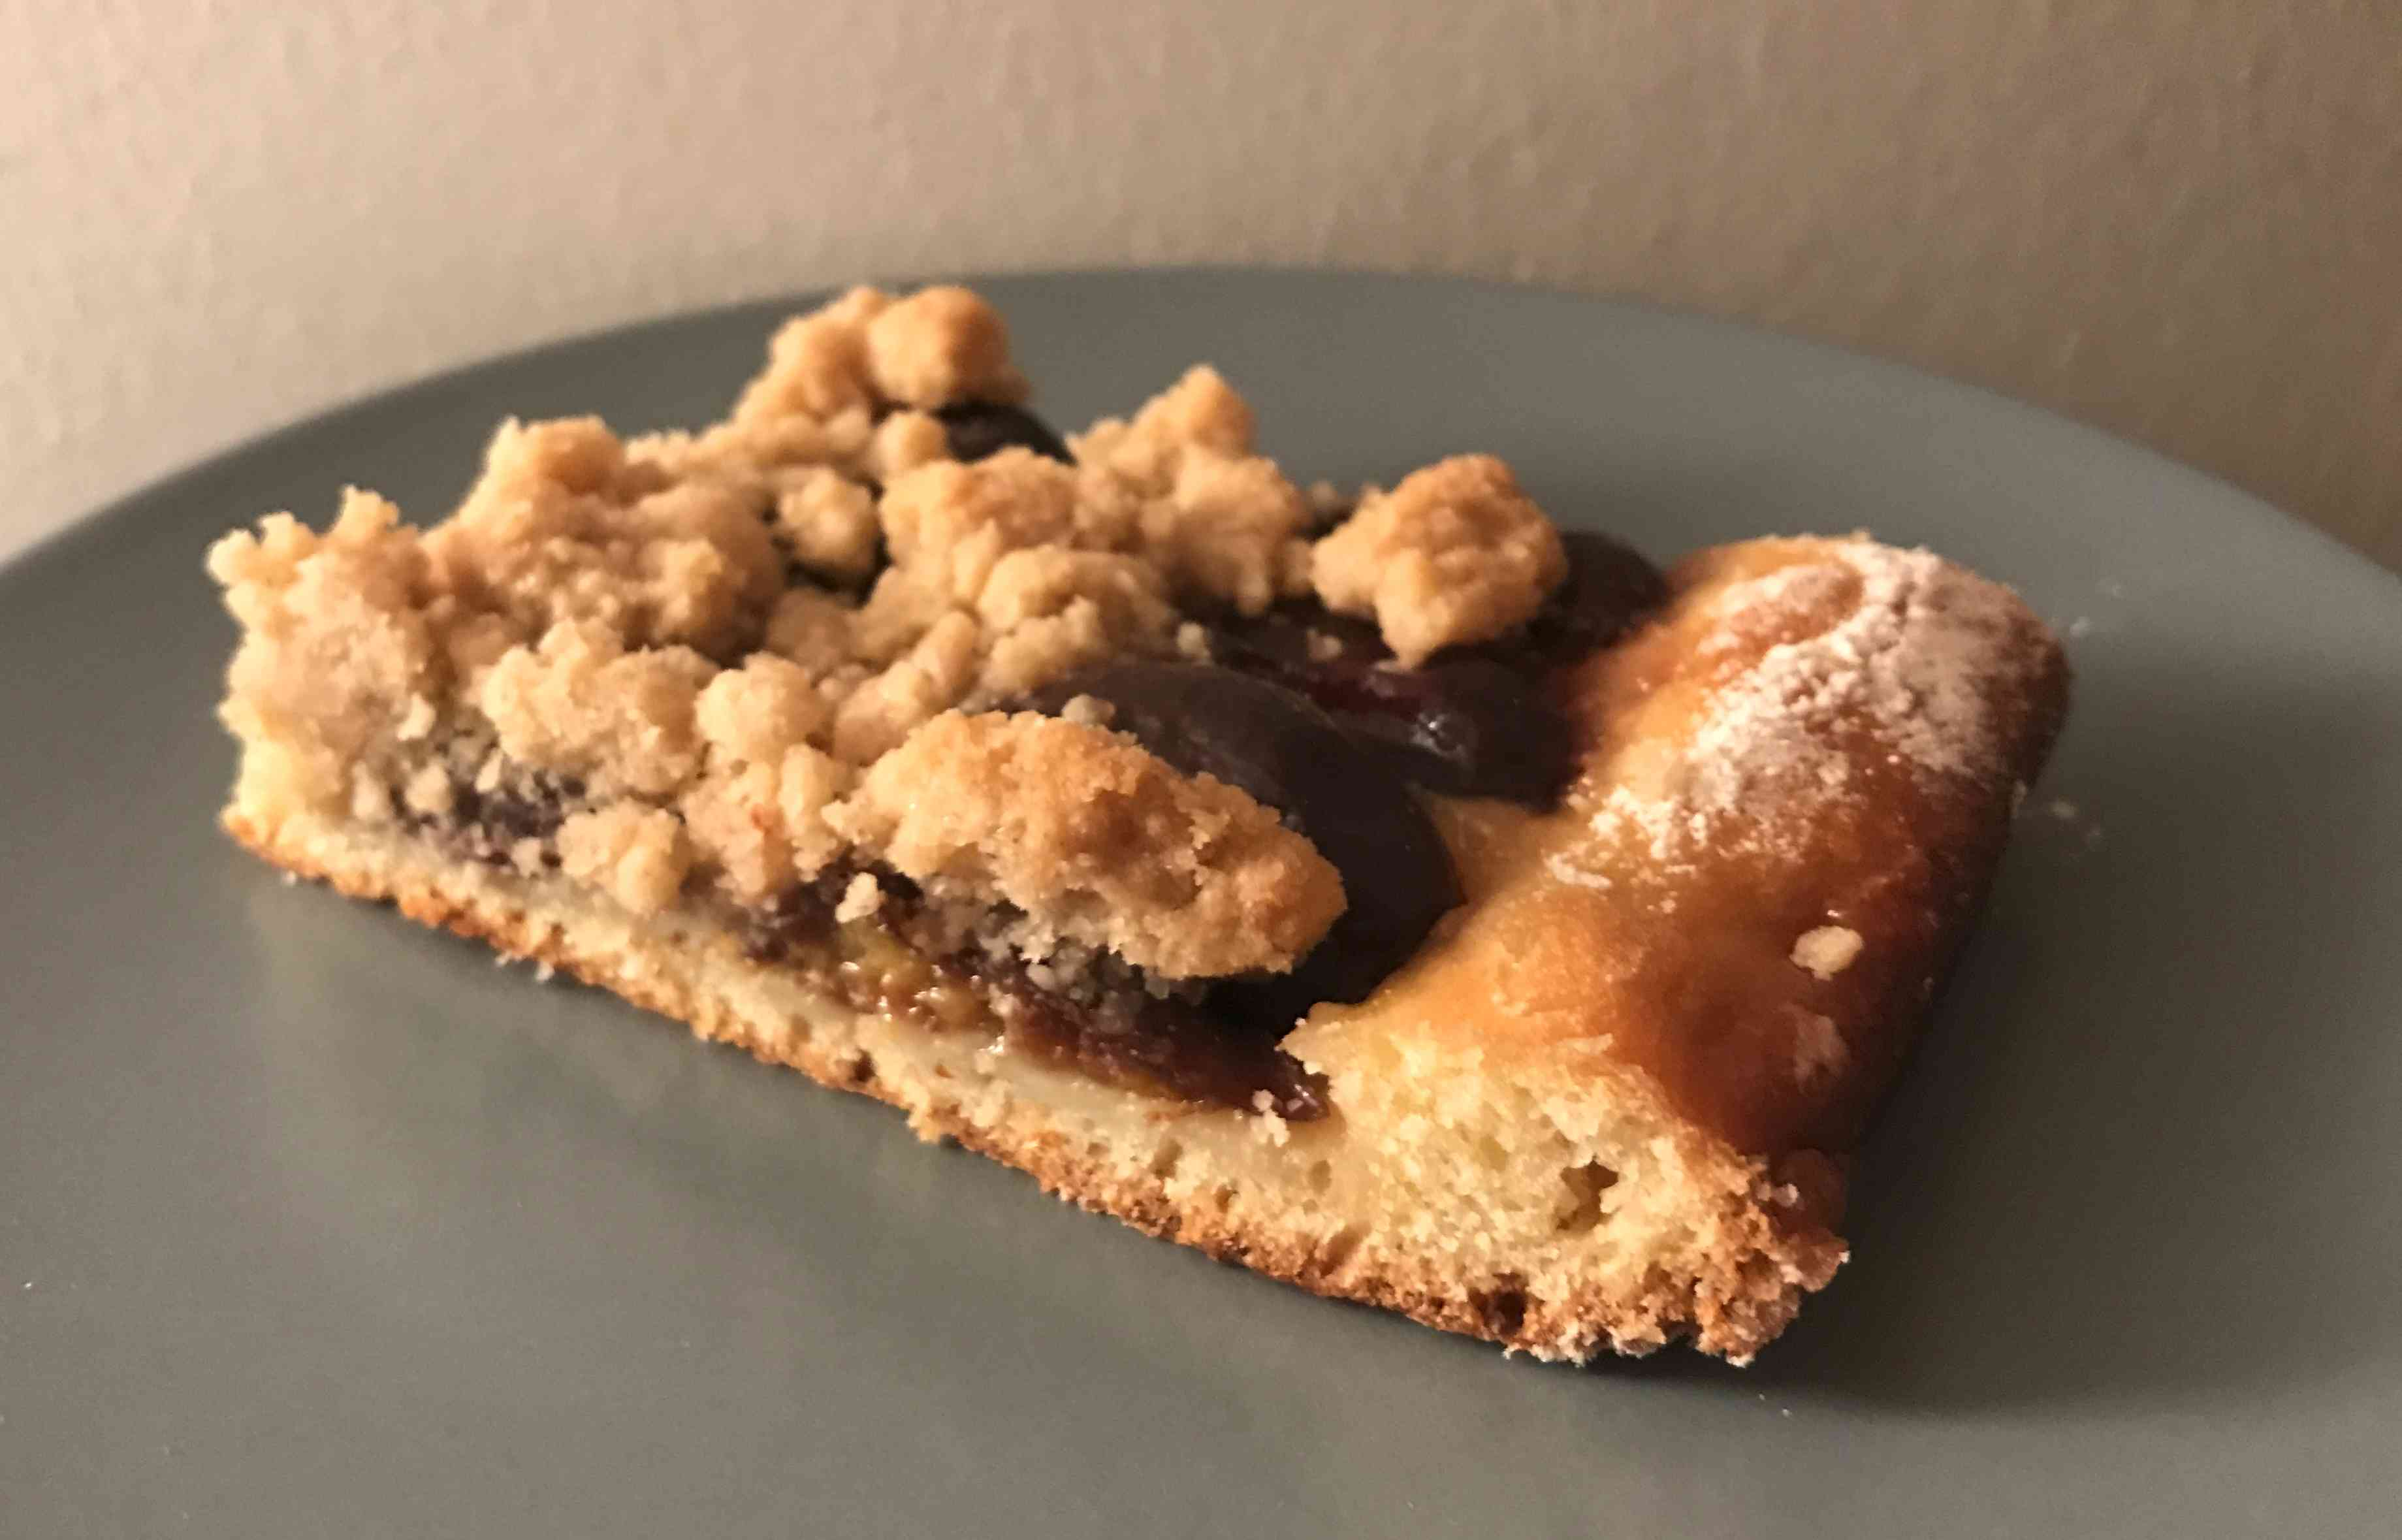
\includegraphics[height = 5cm]{media/pflaumenkuchen_v2.jpg}	\\
									&	\\
			\textbf{Beschreibung}	&	Wenn man im späten Sommer sehr viele Pflaumen auf einmal bekommt lohnt es sich einen saftigen Pflaumenblechkuchen zu backen, wie ich ihn von meinem Vater kenne!\\
									&	\\
			\begin{tabular}[t]{rr}
				\textbf{Zutaten} 			\\
				Für 20-25 Portionen	\\
			\end{tabular}			&	\begin{tabular}[t]{llll}
											Boden: \\

											& 500 g & Weizenmehl, 550er \\
											& 250 ml & Milch \\
											& 80 g & Butter \\
											& 160 g & Zucker \\
											& 2 & Eier \\
											& 4 g & Salz \\
											& 2 g & Trockenhefe \\

											Belag : \\
											& 1 kg & Pflaumen \\
											& 100 g & Zucker \\

											Zimt-Streusel: \\
											& 200 g & Weizenmehl, 550er \\
											& 100 g & Butter \\
											& 100 g & Zucker \\
											& 1 g & Salz \\
											& 1/2 TL & Zimt \\
										\end{tabular} \\ 
			\textbf{Passendes}		&	\begin{itemize}[nosep]
											\item Schlagsahne
										\end{itemize}	\\

			\end{tabularx}
			\newpage
			\begin{tabularx}{\textwidth}{r|L}
			
			\begin{tabular}[t]{rr}
				\textbf{Zubereitung}	\\
				Vorbereitungszeit: 45 min	\\
				Gehzeit: 12-24 h			\\
				Backtemperatur: 200°C		\\
				Backzeit: 20-30 min 
			\end{tabular}			&	\begin{enumerate}[nosep]
											\item Setze mit den Zutaten für den Boden einen süßen Hefeteig analog zu Rezept \ref{Hefezopf} an und lasse ihn gehen.
											\item Wasche, entkerne und halbiere die Pflaumen. Vermische sie mit dem Zucker, sodass sie ihren Saft etwas abgeben.
											\item Bereite die Streusel zu, indem Zucker, Butter, Salz, Zimt und Mehl in dieser Reihenfolge vermischt werden. Lasse auf die Streuselmasse im Kühlschrank stehen um abzukühlen.
											\item Ist der Teig fertig gegangen, gib ordentlich Mehl auf ein Blech gib den Teig für den Boden darauf. Verteile diesen mit den Händen, wobei auch die Oberseite bemehlt werden sollte. 
											\item Verteile die Pflaumen auf der Flächte, wobei die zurückbleibende Flüssigkeit beiseitegestellt werden kann und später hinzugefügt. Forme aus dem Streuselteig mit den Händen die Streusel durch Greifen und verteile auch sie über den ganzen Kuchen.
											\item Backe den Kuchen bei 200°C für 20-30 min, bis der Boden gleichmäßig durch ist und ein guter Bräunungsgrad erreicht ist.
										\end{enumerate}	\\
		\end{tabularx}
		\newpage
		


%----------------------------------<Getränke>--------------------------------------

\chapter{Getränke}

%----------------------------------<Frühstück>--------------------------------------

\chapter{Frühstück}

%------------------------------------------------------------------------
%------------------------------------------------------------------------

\end{document}